\documentclass[]{article}

\usepackage{lmodern}
\usepackage{amssymb,amsmath}
\usepackage{ifxetex,ifluatex}
\usepackage{fixltx2e} % provides \textsubscript
\usepackage[T1]{fontenc}
\usepackage[utf8]{inputenc}
\usepackage{upquote}
\usepackage{microtype}
\usepackage[unicode=true]{hyperref}
\usepackage{longtable,booktabs}
\usepackage{footnote}
\usepackage{listings}
\usepackage{mathtools}
\usepackage{parskip}
\usepackage[margin=0.7in]{geometry}
\usepackage{titlesec}
\usepackage[yyyymmdd,hhmmss]{datetime}
\usepackage{textcomp}
\usepackage{tikz}

\usetikzlibrary{trees}
\tikzstyle{every node}=[draw=black,thick,anchor=west]
\tikzstyle{selected}=[draw=blue]
\tikzstyle{optional}=[dashed,fill=gray!50]

\renewcommand{\dateseparator}{.}

\makeatletter
\newcommand*{\bdiv}{%
  \nonscript\mskip-\medmuskip\mkern5mu%
  \mathbin{\operator@font div}\penalty900\mkern5mu%
  \nonscript\mskip-\medmuskip
}
\makeatother

% Newer LaTeX versions should not add ligatures to listings, but for some reason
% it is not the case for me. As a result select PDF viewers copy wrong data.
\lstdefinestyle{ocbash}{
  language=bash,
  frame=tb,
  columns=fullflexible,
  captionpos=b,
  basicstyle=\ttfamily\normalsize,
  keepspaces=true,
  morekeywords={git, make, build, ioreg, grep, nvram, sort, sudo, diskutil, gfxutil, strings, dd, cut},
  literate =
    {"}{{\textquotedbl}}1
    {'}{{\textquotesingle}}1
    {-}{{-}}1
    {~}{{\texttildelow}}1
    {*}{{*}}1
    {fl}{{f{}l}}2
    {fi}{{f{}i}}2
    ,
}

\UseMicrotypeSet[protrusion]{basicmath} % disable protrusion for tt fonts
\PassOptionsToPackage{hyphens}{url} % url is loaded by hyperref

\makesavenoteenv{long table} % Fix footnotes in tables

% set default figure placement to htbp
\makeatletter
\def\fps@figure{htbp}
\makeatother

\providecommand{\tightlist}{%
  \setlength{\itemsep}{0pt}\setlength{\parskip}{0pt}}

\newcommand{\sectionbreak}{\clearpage}

\begin{document}

\begin{titlepage}
   \begin{center}
       \vspace*{2.0in}

       \Huge

       \IfFileExists{Logos/Logo.pdf}
         {
\includegraphics[width=160pt, height=160pt]{Logos/Logo.pdf}}
         {
\includegraphics[width=160pt, height=160pt]{../Logos/Logo.pdf}}

       \sffamily

       \textbf{OpenCore}

       \vspace{0.2in}

       Reference Manual (0.5.4)

       \vspace{0.2in}

        {[}\today{]}

       \normalsize

       \vfill

       \rmfamily

       Copyright \textcopyright 2018-2019 vit9696

   \end{center}
\end{titlepage}

\tableofcontents

\section{Introduction}\label{introduction}

This document provides information on
\href{https://github.com/acidanthera/OpenCorePkg}{OpenCore} user
configuration file format used to setup the correct functioning of macOS
operating system. It is to be read as the official clarification of expected
OpenCore behaviour. All deviations, if found in published OpenCore releases,
shall be considered documentation or implementation bugs, and are requested to be
reported through \href{https://github.com/acidanthera/bugtracker}{Acidanthera Bugtracker}.
All other sources or translations of this document are unofficial and may contain errors.

This document is structured as a specification, and is not meant to provide a step by
step algorithm for configuring end-user board support package (BSP). Any third-party
articles, tools, books, etc., providing such material are prone to their authors'
preferences, tastes, this document misinterpretation, and essential obsolescence.
In case you still use these sources, for example, 
\href{https://khronokernel-2.gitbook.io/opencore-vanilla-desktop-guide}{Opencore Vanilla Desktop Guide},
please ensure following this document for every made decision and judging its consequences.
Regardless of the sources used you are required to fully understand every dedicated OpenCore
configuration option and concept prior to reporting any issues in
\href{https://github.com/acidanthera/bugtracker}{Acidanthera Bugtracker}.

\subsection{Generic Terms}\label{generic-terms}

\begin{itemize}
\item
  \texttt{plist} --- Subset of ASCII Property List format written in
  XML, also know as XML plist format version 1. Uniform Type Identifier
  (UTI): \texttt{com.apple.property-list}. Plists consist of
  \texttt{plist\ objects}, which are combined to form a hierarchical
  structure. Due to plist format not being well-defined, all the
  definitions of this document may only be applied after plist is
  considered valid by running \texttt{plutil\ -lint}. External
  references: https://www.apple.com/DTDs/PropertyList-1.0.dtd,
  \texttt{man\ plutil}.
\item
  \texttt{plist\ type} --- plist collections (\texttt{plist\ array},
  \texttt{plist\ dictionary}, \texttt{plist\ key}) and primitives
  (\texttt{plist\ string}, \texttt{plist\ data}, \texttt{plist\ date},
  \texttt{plist\ boolean}, \texttt{plist\ integer},
  \texttt{plist\ real}).
\item
  \texttt{plist\ object} --- definite realisation of
  \texttt{plist\ type}, which may be interpreted as value.
\item
  \texttt{plist\ array} --- array-like collection, conforms to
  \texttt{array}. Consists of zero or more \texttt{plist\ objects}.
\item
  \texttt{plist\ dictionary} --- map-like (associative array)
  collection, conforms to \texttt{dict}. Consists of zero or more
  \texttt{plist\ keys}.
\item
  \texttt{plist\ key} --- contains one \texttt{plist\ object} going by
  the name of \texttt{plist\ key}, conforms to \texttt{key}. Consists of
  printable 7-bit ASCII characters.
\item
  \texttt{plist\ string} --- printable 7-bit ASCII string, conforms to
  \texttt{string}.
\item
  \texttt{plist\ data} --- base64-encoded blob, conforms to
  \texttt{data}.
\item
  \texttt{plist\ date} --- ISO-8601 date, conforms to \texttt{date},
  unsupported.
\item
  \texttt{plist\ boolean} --- logical state object, which is either true
  (1) or false (0), conforms to \texttt{true} and \texttt{false}.
\item
  \texttt{plist\ integer} --- possibly signed integer number in base 10,
  conforms to \texttt{integer}. Fits in 64-bit unsigned integer in two's
  complement representation, unless a smaller signed or unsigned
  integral type is explicitly mentioned in specific
  \texttt{plist\ object} description.
\item
  \texttt{plist\ real} --- floating point number, conforms to
  \texttt{real}, unsupported.
\item
  \texttt{plist\ metadata} --- value cast to data by the implementation.
  Permits passing \texttt{plist\ string}, in which case the result is
  represented by a null-terminated sequence of bytes (aka C string),
  \texttt{plist\ integer}, in which case the result is represented by
  \emph{32-bit} little endian sequence of bytes in two's complement
  representation, \texttt{plist\ boolean}, in which case the value is
  one byte: \texttt{01} for \texttt{true} and \texttt{00} for
  \texttt{false}, and \texttt{plist\ data} itself. All other types or
  larger integers invoke undefined behaviour.
\end{itemize}

\section{Configuration}\label{configuration-overview}

\subsection{Configuration Terms}\label{configuration-terms}

\begin{itemize}
\item
  \texttt{OC\ config} --- OpenCore Configuration file in \texttt{plist}
  format named \texttt{config.plist}. It has to provide extensible way
  to configure OpenCore and is structured to be separated into multiple
  named sections situated in the root \texttt{plist\ dictionary}. These
  sections are permitted to have \texttt{plist\ array} or
  \texttt{plist\ dictionary} types and are described in corresponding
  sections of this document.
\item
  \texttt{valid\ key} --- \texttt{plist\ key} object of
  \texttt{OC\ config} described in this document or its future
  revisions. Besides explicitly described \texttt{valid\ keys}, keys
  starting with \texttt{\#} symbol (e.g. \texttt{\#Hello}) are also
  considered \texttt{valid\ keys} and behave as comments, effectively
  discarding their value, which is still required to be a valid
  \texttt{plist\ object}. All other \texttt{plist\ keys} are not valid,
  and their presence yields to \texttt{undefined\ behaviour}.
\item
  \texttt{valid\ value} --- valid \texttt{plist\ object} of
  \texttt{OC\ config} described in this document that matches all the
  additional requirements in specific \texttt{plist\ object} description
  if any.
\item
  \texttt{invalid\ value} --- valid \texttt{plist\ object} of
  \texttt{OC\ config} described in this document that is of other
  \texttt{plist\ type}, does not conform to additional requirements
  found in specific \texttt{plist\ object} description (e.g.~value
  range), or missing from the corresponding collection.
  \texttt{Invalid\ value} is read with or without an error message as
  any possible value of this \texttt{plist\ object} in an undetermined
  manner (i.e.~the values may not be same across the reboots). Whilst
  reading an \texttt{invalid\ value} is equivalent to reading certain
  defined \texttt{valid\ value}, applying incompatible value to the host
  system may yield to \texttt{undefined\ behaviour}.
\item
  \texttt{optional\ value} --- \texttt{valid\ value} of
  \texttt{OC\ config} described in this document that reads in a certain
  defined manner provided in specific \texttt{plist\ object} description
  (instead of \texttt{invalid\ value}) when not present in
  \texttt{OC\ config}. All other cases of \texttt{invalid\ value} do
  still apply. Unless explicitly marked as \texttt{optional\ value}, any
  other value is required to be present and reads to
  \texttt{invalid\ value} if missing.
\item
  \texttt{fatal\ behaviour} --- behaviour leading to boot termination.
  Implementation must stop the boot process from going any further until
  next host system boot. It is allowed but not required to perform cold
  reboot or show any warning message.
\item
  \texttt{undefined\ behaviour} --- behaviour not prescribed by this
  document. Implementation is allowed to take any measures including but
  not limited to \texttt{fatal\ behaviour}, assuming any states or
  values, or ignoring, unless these measures negatively affect system
  security in general.
\end{itemize}

\subsection{Configuration Processing}\label{configuration-processing}

\texttt{OC\ config} is guaranteed to be processed at least once if it
was found. Depending on OpenCore bootstrapping mechanism multiple
\texttt{OC\ config} files may lead to reading any of them. No
\texttt{OC\ Config} may be present on disk, in which case all the values
read follow the rules of \texttt{invalid\ value} and
\texttt{optional\ value}.

\texttt{OC\ config} has size, nesting, and key amount limitations.
\texttt{OC\ config} size does not exceed \texttt{16\ MBs}.
\texttt{OC\ config} has no more than \texttt{8} nesting levels.
\texttt{OC\ config} has up to \texttt{16384} XML nodes (i.e.~one
\texttt{plist\ dictionary} item is counted as a pair of nodes) within
each \texttt{plist\ object}.

Reading malformed \texttt{OC\ config} file leads to
\texttt{undefined\ behaviour}. Examples of malformed \texttt{OC\ config}
cover at least the following cases:

\begin{itemize}
\tightlist
\item
  files non-conformant to \texttt{plist} DTD
\item
  files with unsupported or non-conformant \texttt{plist\ objects} found
  in this document
\item
  files violating size, nesting, and key amount limitations
\end{itemize}

It is recommended but not required to abort loading malformed
\texttt{OC\ config} and continue as if no \texttt{OC\ config} was
present. For forward compatibility it is recommended but not required
for the implementation to warn about the use of
\texttt{invalid\ values}. Recommended practice of interpreting
\texttt{invalid\ values} is to conform to the following convention where
applicable:

\begin{longtable}[]{@{}ll@{}}
\toprule
Type & Value\tabularnewline
\midrule
\endhead
\texttt{plist\ string} & Empty string
(\texttt{\textless{}string\textgreater{}\textless{}/string\textgreater{}})\tabularnewline
\texttt{plist\ data} & Empty data
(\texttt{\textless{}data\textgreater{}\textless{}/data\textgreater{}})\tabularnewline
\texttt{plist\ integer} & 0
(\texttt{\textless{}integer\textgreater{}0\textless{}/integer\textgreater{}})\tabularnewline
\texttt{plist\ boolean} & False
(\texttt{\textless{}false/\textgreater{}})\tabularnewline
\texttt{plist\ tristate} & False
(\texttt{\textless{}false/\textgreater{}})\tabularnewline
\bottomrule
\end{longtable}

\subsection{Configuration Structure}\label{configuration-structure}

\texttt{OC\ config} is separated into following sections, which are described
in separate sections of this document. By default it is tried to not enable
anything and optionally provide kill switches with \texttt{Enable} property
for \texttt{plist dict} entries. In general the configuration is written
idiomatically to group similar actions in subsections:

\begin{itemize}
\tightlist
\item
  \texttt{Add} provides support for data addition.
\item
  \texttt{Block} provides support for data removal or ignorance.
\item
  \texttt{Patch} provides support for data modification.
\item
  \texttt{Quirks} provides support for specific hacks.
\end{itemize}

Root configuration entries consist of the following:

\begin{itemize}
\tightlist
\item
  \hyperref[acpi]{\texttt{ACPI}}
\item
  \hyperref[booter]{\texttt{Booter}}
\item
  \hyperref[devprops]{\texttt{DeviceProperties}}
\item
  \hyperref[kernel]{\texttt{Kernel}}
\item
  \hyperref[misc]{\texttt{Misc}}
\item
  \hyperref[nvram]{\texttt{NVRAM}}
\item
  \hyperref[platforminfo]{\texttt{PlatformInfo}}
\item
  \hyperref[uefi]{\texttt{UEFI}}
\end{itemize}

\emph{Note}: Currently most properties try to have defined values even if not
specified in the configuration for safety reasons. This behaviour should not
be relied upon, and all fields must be properly specified in the configuration.

\section{Setup}\label{setup-overview}

\subsection{Directory Structure}\label{directory-structure}

\begin{center}
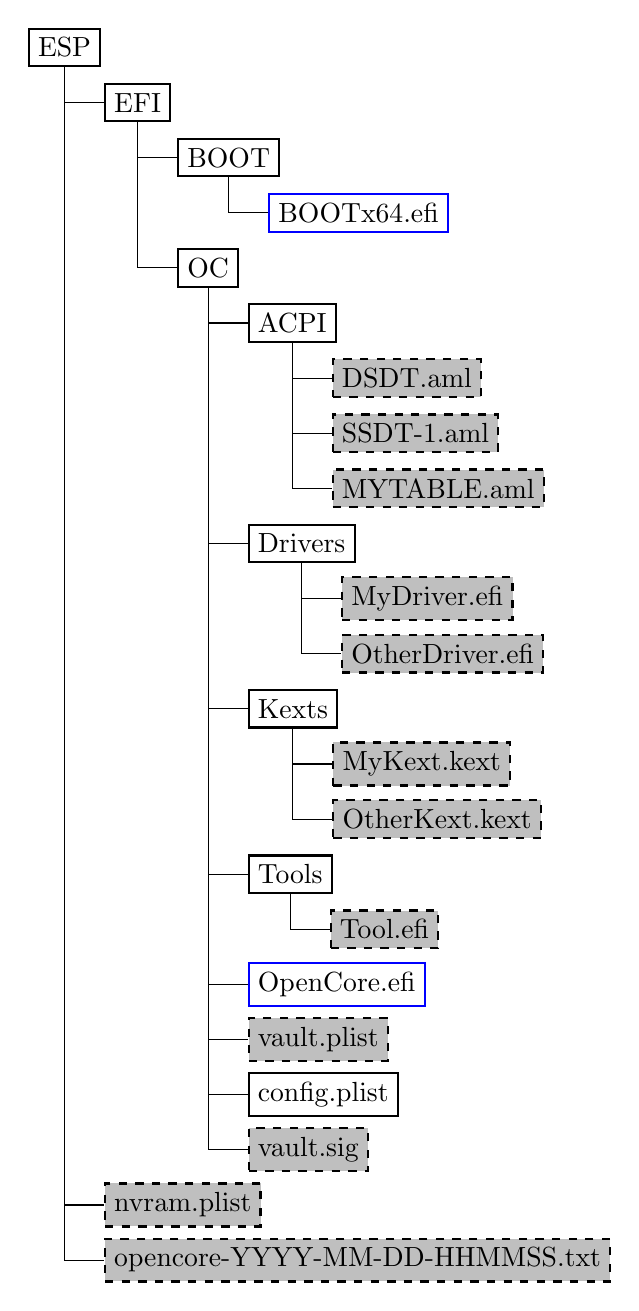
\begin{tikzpicture}[%
  grow via three points={one child at (0.5,-0.7) and
  two children at (0.5,-0.7) and (0.5,-1.4)},
  edge from parent path={(\tikzparentnode.south) |- (\tikzchildnode.west)}]
  \node {ESP}
    child { node {EFI}
      child { node {BOOT}
        child { node [selected] {BOOTx64.efi}}
      }
      child [missing] {}
      child { node {OC}
        child { node {ACPI}
          child { node [optional] {DSDT.aml}}
          child { node [optional] {SSDT-1.aml}}
          child { node [optional] {MYTABLE.aml}}
        }
        child [missing] {}
        child [missing] {}
        child [missing] {}
        child { node {Drivers}
          child { node [optional] {MyDriver.efi}}
          child { node [optional] {OtherDriver.efi}}
        }
        child [missing] {}
        child [missing] {}
        child { node {Kexts}
          child { node [optional] {MyKext.kext}}
          child { node [optional] {OtherKext.kext}}
        }
        child [missing] {}
        child [missing] {}
        child { node  {Tools}
          child { node [optional] {Tool.efi}}
        }
        child [missing] {}
        child { node [selected] {OpenCore.efi}}
        child { node [optional] {vault.plist}}
        child { node {config.plist}}
        child { node [optional] {vault.sig}}
      }
    }
    child [missing] {}
    child [missing] {}
    child [missing] {}
    child [missing] {}
    child [missing] {}
    child [missing] {}
    child [missing] {}
    child [missing] {}
    child [missing] {}
    child [missing] {}
    child [missing] {}
    child [missing] {}
    child [missing] {}
    child [missing] {}
    child [missing] {}
    child [missing] {}
    child [missing] {}
    child [missing] {}
    child [missing] {}
    child { node [optional] {nvram.plist}}
    child { node [optional] {opencore-YYYY-MM-DD-HHMMSS.txt}}
  ;
\end{tikzpicture}
\break
\label{fig:DS}
Figure 1. Directory Structure
\end{center}

When directory boot is used the directory structure used should follow
the description on \hyperref[fig:DS]{Directory Structure} figure. Available
entries include:

\begin{itemize}
\tightlist
\item
  \texttt{BOOTx64.efi}
  \break
  Initial booter, which loads \texttt{OpenCore.efi} unless it was
  already started as a driver.
\item
  \texttt{ACPI}
  \break
  Directory used for storing supplemental ACPI information
  for \hyperref[acpi]{\texttt{ACPI}} section.
\item
  \texttt{Drivers}
  \break
  Directory used for storing supplemental \texttt{UEFI}
  drivers for \hyperref[uefi]{\texttt{UEFI}} section.
\item
  \texttt{Kexts}
  \break
  Directory used for storing supplemental kernel information
  for \hyperref[kernel]{\texttt{Kernel}} section.
\item
  \texttt{Tools}
  \break
  Directory used for storing supplemental tools.
\item
  \texttt{OpenCore.efi}
  \break
  Main booter driver responsible for operating system loading.
\item
  \texttt{vault.plist}
  \break
  Hashes for all files potentially loadable by \texttt{OC Config}.
\item
  \texttt{config.plist}
  \break
  \texttt{OC Config}.
\item
  \texttt{vault.sig}
  \break
  Signature for \texttt{vault.plist}.
\item
  \texttt{nvram.plist}
  \break
  OpenCore variable import file.
\item
  \texttt{opencore-YYYY-MM-DD-HHMMSS.txt}
  \break
  OpenCore log file.
\end{itemize}

\subsection{Installation and Upgrade}\label{configuration-install}

To install OpenCore reflect the
\hyperref[configuration-structure]{Configuration Structure} described
in the previous section on a EFI volume of a GPT partition. While
corresponding sections of this document do provide some information
in regards to external resources like ACPI tables, UEFI drivers,
or kernel extensions (kexts), completeness of the matter is out of
the scope of this document. Information about kernel extensions may
be found in a separate
\href{https://github.com/acidanthera/OpenCorePkg/blob/master/Docs/Kexts.md}{Kext List}
document available in OpenCore repository. Vaulting information is provided in
\hyperref[miscsecurityprops]{Security Properties} section of this document.

\texttt{OC\ config}, just like any property lists can be edited with any
stock textual editor (e.g. nano, vim), but specialised software may provide
better experience. On macOS the preferred GUI application is
\href{https://developer.apple.com/xcode}{Xcode}. For a lightweight
cross-platform and open-source alternative
\href{https://github.com/corpnewt/ProperTree}{ProperTree} editor can be
utilised.

For BIOS booting a third-party UEFI environment provider will have to
be used. \texttt{DuetPkg} is one of the known UEFI environment providers
for legacy systems. To run OpenCore on such a legacy system you can install
\texttt{DuetPkg} with a dedicated tool:
\href{https://github.com/acidanthera/OcSupportPkg/tree/master/Utilities/BootInstall}{BootInstall}.

For upgrade purposes refer to \texttt{Differences.pdf} document, providing
the information about the changes affecting the configuration compared
to the previous release, and \texttt{Changelog.md} document, containing
the list of modifications across all published updates.

\subsection{Contribution}\label{configuration-comp}

OpenCore can be compiled as an ordinary
\href{https://github.com/tianocore/tianocore.github.io/wiki/EDK-II}{EDK II}.
Since \href{https://github.com/tianocore/tianocore.github.io/wiki/UDK}{UDK}
development was abandoned by TianoCore, OpenCore requires the use of
\href{https://github.com/tianocore/tianocore.github.io/wiki/EDK-II#stable-tags}{EDK II Stable}.
Currently supported EDK II release (potentially with patches enhancing the experience)
is hosted in \href{https://github.com/acidanthera/audk}{acidanthera/audk}.

The only officially supported toolchain is \texttt{XCODE5}. Other toolchains
might work, but are neither supported, nor recommended. Contribution of clean
patches is welcome. Please do follow
\href{https://github.com/tianocore/tianocore.github.io/wiki/Code-Style-C}{EDK II C Codestyle}.

Required external package dependencies include
\href{https://github.com/acidanthera/OcSupportPkg}{EfiPkg},
\href{https://github.com/acidanthera/OcSupportPkg}{MacInfoPkg}, and
\href{https://github.com/acidanthera/OcSupportPkg}{OcSupportPkg}.

To compile with \texttt{XCODE5}, besides \href{https://developer.apple.com/xcode}{Xcode},
one should also install \href{https://www.nasm.us}{NASM} and
\href{https://github.com/acidanthera/ocbuild/raw/master/external/mtoc-mac64.zip}{MTOC}.
The latest Xcode version is recommended for use despite the toolchain name. Example
command sequence may look as follows:

\begin{lstlisting}[caption=Compilation Commands, label=compile, style=ocbash]
git clone https://github.com/acidanthera/audk UDK
cd UDK
git clone https://github.com/acidanthera/EfiPkg
git clone https://github.com/acidanthera/MacInfoPkg
git clone https://github.com/acidanthera/OcSupportPkg
git clone https://github.com/acidanthera/OpenCorePkg
source edksetup.sh
make -C BaseTools
build -a X64 -b RELEASE -t XCODE5 -p OpenCorePkg/OpenCorePkg.dsc
\end{lstlisting}

For IDE usage Xcode projects are available in the root of the repositories. Another
approach could be \href{https://www.sublimetext.com}{Sublime Text} with
\href{https://niosus.github.io/EasyClangComplete}{EasyClangComplete} plugin.
Add \texttt{.clang\_complete} file with similar content to your UDK root:

\begin{lstlisting}[caption=ECC Configuration, label=eccfile, style=ocbash]
-I/UefiPackages/MdePkg
-I/UefiPackages/MdePkg/Include
-I/UefiPackages/MdePkg/Include/X64
-I/UefiPackages/EfiPkg
-I/UefiPackages/EfiPkg/Include
-I/UefiPackages/EfiPkg/Include/X64
-I/UefiPackages/AppleSupportPkg/Include
-I/UefiPackages/OpenCorePkg/Include
-I/UefiPackages/OcSupportPkg/Include
-I/UefiPackages/MacInfoPkg/Include
-I/UefiPackages/UefiCpuPkg/Include
-IInclude
-include
/UefiPackages/MdePkg/Include/Uefi.h
-fshort-wchar
-Wall
-Wextra
-Wno-unused-parameter
-Wno-missing-braces
-Wno-missing-field-initializers
-Wno-tautological-compare
-Wno-sign-compare
-Wno-varargs
-Wno-unused-const-variable
-DOC_TARGET_NOOPT=1
\end{lstlisting}

\textbf{Warning}: Tool developers modifying \texttt{config.plist} or any other OpenCore
files must ensure that their tool checks for \texttt{opencore-version} NVRAM variable
(see \hyperref[miscdebugprops]{Debug Properties} section below) and warn the user
if the version listed is unsupported or prerelease. OpenCore configuration may change
across the releases and the tool shall ensure that it carefully follows this document.
Failure to do so may result in this tool to be considered as malware and blocked with
all possible means.

\subsection{Coding conventions}\label{configuration-conv}

Just like any other project we have conventions that we follow during the development.
All third-party contributors are highly recommended to read and follow the conventions
listed below before submitting their patches. In general it is also recommended to firstly
discuss the issue in \href{https://github.com/acidanthera/bugtracker}{Acidanthera Bugtracker}
before sending the patch to ensure no double work and to avoid your patch being rejected.

\textbf{Organisation}. The codebase is structured in multiple repositories
which contain separate EDK II packages. \texttt{AppleSupportPkg} and \texttt{OpenCorePkg}
are primary packages, and \texttt{EfiPkg}, \texttt{OcSupportPkg}, \texttt{MacInfoPkg.dsc})
are dependent packages.
\begin{itemize}
\tightlist
\item Whenever changes are required in multiple repositories, separate pull requests should
be sent to each.
\item Committing the changes should happen firstly to dependent repositories, secondly to
primary repositories to avoid automatic build errors.
\item Each unique commit should compile with \texttt{XCODE5} and preferably with other
toolchains. In the majority of the cases it can be checked by accessing the
\href{https://travis-ci.com/acidanthera}{CI interface}. Ensuring that static analysis finds
no warnings is preferred.
\item External pull requests and tagged commits must be validated. That said, commits in
master may build but may not necessarily work.
\item Internal branches should be named as follows: \texttt{author-name-date}, e.g.
\texttt{vit9696-ballooning-20191026}.
\item Commit messages should be prefixed with the primary module (e.g. library or code module) the
changes were made in. For example, \texttt{OcGuardLib: Add OC\_ALIGNED macro}. For non-library changes
\texttt{Docs} or \texttt{Build} prefixes are used.
\end{itemize}

\textbf{Design}. The codebase is written in a subset of freestanding C11 (C17) supported by
most modern toolchains used by EDK II. Applying common software development practices or requesting
clarification is recommended if any particular case is not discussed below.
\begin{itemize}
\tightlist
\item Never rely on undefined behaviour and try to avoid implementation defined behaviour unless
explicitly covered below (feel free to create an issue when a relevant case is not present).
\item Use \texttt{OcGuardLib} to ensure safe integral arithmetics avoiding overflows. Unsigned
wraparound should be relied on with care and reduced to the necessary amount.
\item Check pointers for correct alignment with \texttt{OcGuardLib} and do not rely on the architecture
being able to dereference unaligned pointers.
\item Use flexible array members instead of zero-length or one-length arrays where necessary.
\item Use static assertions (\texttt{STATIC\_ASSERT}) for type and value assumptions, and runtime
assertions (\texttt{ASSERT}) for precondition and invariant sanity checking. Do not use runtime
assertions to check for errors as they should never alter control flow and potentially be excluded.
\item Assume \texttt{UINT32}/\texttt{INT32} to be \texttt{int}-sized and use \texttt{\%u},
\texttt{\%d}, and \texttt{\%x} to print them.
\item Assume \texttt{UINTN}/\texttt{INTN} to be of unspecified size, and cast them to
\texttt{UINT64}/\texttt{INT64} for printing with \texttt{\%Lu}, \texttt{\%Ld} and so on as normal.
\item Do not rely on integer promotions for numeric literals. Use explicit casts when the type is
implementation-dependent or suffixes when type size is known. Assume \texttt{U} for \texttt{UINT32}
and \texttt{ULL} for \texttt{UINT64}.
\item Do ensure unsigned arithmetics especially in bitwise maths, shifts in particular.
\item \texttt{sizeof} operator should take variables instead of types where possible to be error prone.
Use \texttt{ARRAY\_SIZE} to obtain array size in elements. Use \texttt{L\_STR\_LEN} and
\texttt{L\_STR\_SIZE} macros from \texttt{OcStringLib} to obtain string literal sizes to ensure compiler
optimisation.
\item Do not use \texttt{goto} keyword. Prefer early \texttt{return}, \texttt{break}, or \texttt{continue}
after failing to pass error checking instead of nesting conditionals.
\item Use \texttt{EFIAPI}, force UEFI calling convention, only in protocols, external callbacks between
modules, and functions with variadic arguments.
\item Provide inline documentation to every added function, at least describing its inputs, outputs,
precondition, postcondition, and giving a brief description.
\item Do not use \texttt{RETURN\_STATUS}. Assume \texttt{EFI\_STATUS} to be a matching superset that is
to be always used when \texttt{BOOLEAN} is not enough.
\item Security violations should halt the system or cause a forced reboot.
\end{itemize}

\textbf{Codestyle}. The codebase follows
\href{https://github.com/tianocore/tianocore.github.io/wiki/Code-Style-C}{EDK II codestyle} with few changes
and clarifications.
\begin{itemize}
\tightlist
\item Write inline documentation for the functions and variables only once: in headers, where a header prototype
is available, and inline for \texttt{static} variables and functions.
\item Use line length of 120 characters or less, preferably 100 characters.
\item Use spaces after casts, e.g. \texttt{(VOID *)(UINTN) Variable}.
\item Use SPDX license headers as shown in
\href{https://github.com/acidanthera/bugtracker/issues/483}{acidanthera/bugtracker\#483}.
\end{itemize}

\textbf{Debugging}. The codebase incorporates EDK II debugging and few custom features to improve the experience.
\begin{itemize}
\tightlist
\item Use module prefixes, 2-5 letters followed by a colon (\texttt{:}), for debug messages. For \texttt{OpenCorePkg}
use \texttt{OC:}, for libraries and drivers use their own unique prefixes.
\item Do not use dots (\texttt{.}) in the end of debug messages and separate \texttt{EFI\_STATUS}, printed by
\texttt{\%r}, with a hyphen (e.g. \texttt{OCRAM: Allocation of \%u bytes failed - \%r\textbackslash n}).
\item Use \texttt{DEBUG\_CODE\_BEGIN ()} and \texttt{DEBUG\_CODE\_END ()} constructions to guard debug checks
that may potentially reduce the performance of release builds and are otherwise unnecessary.
\item Use \texttt{DEBUG} macro to print debug messages during normal functioning, and \texttt{RUNTIME\_DEBUG} for
debugging after \texttt{EXIT\_BOOT\_SERVICES}. 
\item Use \texttt{DEBUG\_VERBOSE} debug level to leave debug messages for future debugging of the code, which
are currently not necessary. By default \texttt{DEBUG\_VERBOSE} messages are ignored even in \texttt{DEBUG} builds.
\item Use \texttt{DEBUG\_INFO} debug level for all non critical messages (including errors) and \texttt{DEBUG\_BULK\_INFO}
for extensive messages that should not appear in NVRAM log that is heavily limited in size. These messages are ignored in
\texttt{RELEASE} builds.
\item Use \texttt{DEBUG\_ERROR} to print critical human visible messages that may potentially halt the boot process, and
\texttt{DEBUG\_WARN} for all other human visible errors, \texttt{RELEASE} builds included.
\end{itemize}

\section{ACPI}\label{acpi}

\subsection{Introduction}\label{acpiintro}

ACPI (Advanced Configuration and Power Interface) is an open standard to
discover and configure computer hardware.
\href{https://uefi.org/specifications}{ACPI specification} defines the
standard tables (e.g.~\texttt{DSDT}, \texttt{SSDT}, \texttt{FACS}, \texttt{DMAR})
and various methods (e.g. \texttt{\_DSM}, \texttt{\_PRW}) for implementation.
Modern hardware needs little changes to maintain ACPI compatibility, yet
some of those are provided as a part of OpenCore.

To compile and disassemble ACPI tables \href{https://github.com/acpica/acpica}{iASL compiler}
can be used developed by \href{https://www.acpica.org}{ACPICA}. GUI front-end to iASL compiler
can be downloaded from \href{https://github.com/acidanthera/MaciASL/releases}{Acidanthera/MaciASL}.

\subsection{Properties}\label{acpiprops}

\begin{enumerate}
\item
  \texttt{Add}\\
  \textbf{Type}: \texttt{plist\ array}\\
  \textbf{Failsafe}: Empty\\
  \textbf{Description}: Load selected tables from \texttt{OC/ACPI}
  directory.

  Designed to be filled with \texttt{plist\ dict} values, describing each block entry.
  See \hyperref[acpipropsadd]{Add Properties} section below.

\item
  \texttt{Block}\\
  \textbf{Type}: \texttt{plist\ array}\\
  \textbf{Failsafe}: Empty\\
  \textbf{Description}: Remove selected tables from ACPI stack.

  Designed to be filled with \texttt{plist\ dict} values, describing each block entry.
  See \hyperref[acpipropsblock]{Block Properties} section below.

\item
  \texttt{Patch}\\
  \textbf{Type}: \texttt{plist\ array}\\
  \textbf{Failsafe}: Empty\\
  \textbf{Description}: Perform binary patches in ACPI tables before
  table addition or removal.

  Designed to be filled with \texttt{plist\ dictionary} values describing each
  patch entry. See \hyperref[acpipropspatch]{Patch Properties} section below.

\item
  \texttt{Quirks}\\
  \textbf{Type}: \texttt{plist\ dict}\\
  \textbf{Description}: Apply individual ACPI quirks described
  in \hyperref[acpipropsquirks]{Quirks Properties} section below.

\end{enumerate}

\subsection{Add Properties}\label{acpipropsadd}

\begin{enumerate}
\item
  \texttt{Comment}\\
  \textbf{Type}: \texttt{plist\ string}\\
  \textbf{Failsafe}: Empty string\\
  \textbf{Description}: Arbitrary ASCII string used to provide human readable
  reference for the entry. It is implementation defined whether this value is
  used.

\item
  \texttt{Enabled}\\
  \textbf{Type}: \texttt{plist\ boolean}\\
  \textbf{Failsafe}: \texttt{false}\\
  \textbf{Description}: This ACPI table will not be added unless set to
  \texttt{true}.

\item
  \texttt{Path}\\
  \textbf{Type}: \texttt{plist\ string}\\
  \textbf{Failsafe}: Empty string\\
  \textbf{Description}: File paths meant to be loaded as ACPI tables.
  Example values include \texttt{DSDT.aml}, \texttt{SubDir/SSDT-8.aml},
  \texttt{SSDT-USBX.aml}, etc.

  ACPI table load order follows the item order in the array. All ACPI tables
  load from \texttt{OC/ACPI} directory.

  \textbf{Note}: All tables but tables with \texttt{DSDT} table identifier
  (determined by parsing data not by filename) insert new tables into ACPI stack.
  \texttt{DSDT}, unlike the rest, performs replacement of DSDT table.

\end{enumerate}

\subsection{Block Properties}\label{acpipropsblock}

\begin{enumerate}
\item
  \texttt{All}\\
  \textbf{Type}: \texttt{plist\ boolean}\\
  \textbf{Failsafe}: \texttt{false}\\
  \textbf{Description}: If set to \texttt{true}, all ACPI tables matching the
  condition will be dropped. Otherwise only first matched table.

\item
  \texttt{Comment}\\
  \textbf{Type}: \texttt{plist\ string}\\
  \textbf{Failsafe}: Empty string\\
  \textbf{Description}: Arbitrary ASCII string used to provide human readable
  reference for the entry. It is implementation defined whether this value is
  used.

\item
  \texttt{Enabled}\\
  \textbf{Type}: \texttt{plist\ boolean}\\
  \textbf{Failsafe}: \texttt{false}\\
  \textbf{Description}: This ACPI table will not be removed unless set to
  \texttt{true}.

\item
  \texttt{OemTableId}\\
  \textbf{Type}: \texttt{plist\ data}, 8 bytes\\
  \textbf{Failsafe}: All zero\\
  \textbf{Description}: Match table OEM ID to be equal to this value
  unless all zero.

\item
  \texttt{TableLength}\\
  \textbf{Type}: \texttt{plist\ integer}\\
  \textbf{Failsafe}: \texttt{0}\\
  \textbf{Description}: Match table size to be equal to this value
  unless \texttt{0}.

\item
  \texttt{TableSignature}\\
  \textbf{Type}: \texttt{plist\ data}, 4 bytes\\
  \textbf{Failsafe}: All zero\\
  \textbf{Description}: Match table signature to be equal to this value
  unless all zero.

  \emph{Note}: Make sure not to specify table signature when the sequence
  needs to be replaced in multiple places. Especially when performing
  different kinds of renames.

\end{enumerate}

\subsection{Patch Properties}\label{acpipropspatch}

\begin{enumerate}

\item
  \texttt{Comment}\\
  \textbf{Type}: \texttt{plist\ string}\\
  \textbf{Failsafe}: Empty string\\
  \textbf{Description}: Arbitrary ASCII string used to provide human readable
  reference for the entry. It is implementation defined whether this value is
  used.

\item
  \texttt{Count}\\
  \textbf{Type}: \texttt{plist\ integer}\\
  \textbf{Failsafe}: \texttt{0}\\
  \textbf{Description}: Number of patch occurrences to apply. \texttt{0} applies
  the patch to all occurrences found.

\item
  \texttt{Enabled}\\
  \textbf{Type}: \texttt{plist\ boolean}\\
  \textbf{Failsafe}: \texttt{false}\\
  \textbf{Description}: This ACPI patch will not be used unless set to
  \texttt{true}.

\item
  \texttt{Find}\\
  \textbf{Type}: \texttt{plist\ data}\\
  \textbf{Failsafe}: Empty data\\
  \textbf{Description}: Data to find. Must equal to \texttt{Replace} in size.

\item
  \texttt{Limit}\\
  \textbf{Type}: \texttt{plist\ integer}\\
  \textbf{Failsafe}: \texttt{0}\\
  \textbf{Description}: Maximum number of bytes to search for. Can be set to
  \texttt{0} to look through the whole ACPI table.

\item
  \texttt{Mask}\\
  \textbf{Type}: \texttt{plist\ data}\\
  \textbf{Failsafe}: Empty data\\
  \textbf{Description}: Data bitwise mask used during find comparison.
  Allows fuzzy search by ignoring not masked (set to zero) bits. Can be
  set to empty data to be ignored. Must equal to \texttt{Replace} in size
  otherwise.

\item
  \texttt{OemTableId}\\
  \textbf{Type}: \texttt{plist\ data}, 8 bytes\\
  \textbf{Failsafe}: All zero\\
  \textbf{Description}: Match table OEM ID to be equal to this value
  unless all zero.

\item
  \texttt{Replace}\\
  \textbf{Type}: \texttt{plist\ data}\\
  \textbf{Failsafe}: Empty data\\
  \textbf{Description}: Replacement data of one or more bytes.

\item
  \texttt{ReplaceMask}\\
  \textbf{Type}: \texttt{plist\ data}\\
  \textbf{Failsafe}: Empty data\\
  \textbf{Description}: Data bitwise mask used during replacement.
  Allows fuzzy replacement by updating masked (set to non-zero) bits. Can be
  set to empty data to be ignored. Must equal to \texttt{Replace} in size
  otherwise.

\item
  \texttt{Skip}\\
  \textbf{Type}: \texttt{plist\ integer}\\
  \textbf{Failsafe}: \texttt{0}\\
  \textbf{Description}: Number of found occurrences to be skipped before replacement
  is done.

\item
  \texttt{TableLength}\\
  \textbf{Type}: \texttt{plist\ integer}\\
  \textbf{Failsafe}: \texttt{0}\\
  \textbf{Description}: Match table size to be equal to this value
  unless \texttt{0}.

\item
  \texttt{TableSignature}\\
  \textbf{Type}: \texttt{plist\ data}, 4 bytes\\
  \textbf{Failsafe}: All zero\\
  \textbf{Description}: Match table signature to be equal to this value
  unless all zero.

\end{enumerate}

In the majority of the cases ACPI patches are not useful and harmful:

\begin{itemize}
\item
  Avoid renaming devices with ACPI patches. This may fail or perform
  improper renaming of unrelated devices (e.g. \texttt{EC} and
  \texttt{EC0}), be unnecessary, or even fail to rename devices in select tables. For
  ACPI consistency it is much safer to rename devices at I/O Registry
  level, as done by
  \href{https://github.com/acidanthera/WhateverGreen}{WhateverGreen}.
\item
  Avoid patching \texttt{\_OSI} to support a higher level of feature sets
  unless absolutely required. Commonly this enables a number of hacks on APTIO
  firmwares, which result in the need to add more patches. Modern firmwares
  generally do not need it at all, and those that do are fine with much
  smaller patches.
\item
  Try to avoid hacky changes like renaming \texttt{\_PRW} or \texttt{\_DSM}
  whenever possible.
\end{itemize}

Several cases, where patching actually does make sense, include:

\begin{itemize}
\item
  Refreshing \texttt{HPET} (or another device) method header to avoid
  compatibility checks by \texttt{\_OSI} on legacy hardware. \texttt{\_STA}
  method with \texttt{if ((OSFL () == Zero)) \{ If (HPTE)  ...  Return (Zero)}
  content may be forced to always return 0xF by replacing
  \texttt{A0 10 93 4F 53 46 4C 00} with \texttt{A4 0A 0F A3 A3 A3 A3 A3}.
\item
  To provide custom method implementation with in an SSDT, for instance,
  to report functional key presses on a laptop, the original method can be replaced
  with a dummy name by patching \texttt{\_Q11} with \texttt{XQ11}.
\end{itemize}

Tianocore \href{https://github.com/tianocore/edk2/blob/UDK2018/MdePkg/Include/IndustryStandard/AcpiAml.h}{AcpiAml.h}
source file may help understanding ACPI opcodes.

\subsection{Quirks Properties}\label{acpipropsquirks}

\begin{enumerate}

\item
  \texttt{FadtEnableReset}\\
  \textbf{Type}: \texttt{plist\ boolean}\\
  \textbf{Failsafe}: \texttt{false}\\
  \textbf{Description}: Provide reset register and flag in FADT table to enable
  reboot and shutdown on legacy hardware. Not recommended unless required.

\item
  \texttt{NormalizeHeaders}\\
  \textbf{Type}: \texttt{plist\ boolean}\\
  \textbf{Failsafe}: \texttt{false}\\
  \textbf{Description}: Cleanup ACPI header fields to workaround macOS
  ACPI implementation bug causing boot crashes. Reference:
  \href{https://alextjam.es/debugging-appleacpiplatform/}{Debugging
  AppleACPIPlatform on 10.13} by Alex James aka theracermaster. The
  issue is fixed in macOS Mojave (10.14).

\item
  \texttt{RebaseRegions}\\
  \textbf{Type}: \texttt{plist\ boolean}\\
  \textbf{Failsafe}: \texttt{false}\\
  \textbf{Description}: Attempt to heuristically relocate ACPI memory
  regions. Not recommended.

  ACPI tables are often generated dynamically by underlying firmware
  implementation. Among the position-independent code, ACPI tables may
  contain physical addresses of MMIO areas used for device
  configuration, usually grouped in regions (e.g.
  \texttt{OperationRegion}). Changing firmware settings or hardware
  configuration, upgrading or patching the firmware inevitably leads to
  changes in dynamically generated ACPI code, which sometimes lead to
  the shift of the addresses in aforementioned \texttt{OperationRegion}
  constructions.

  For this reason it is very dangerous to apply any kind of
  modifications to ACPI tables. The most reasonable approach is to make
  as few as possible changes to ACPI and try to not replace any tables,
  especially DSDT. When this is not possible, then at least attempt to
  ensure that custom DSDT is based on the most recent DSDT or remove
  writes and reads for the affected areas.

  When nothing else helps this option could be tried to avoid stalls at
  \texttt{PCI\ Configuration\ Begin} phase of macOS booting by
  attempting to fix the ACPI addresses. It does not do magic, and only
  works with most common cases. Do not use unless absolutely required.

\item
  \texttt{ResetHwSig}\\
  \textbf{Type}: \texttt{plist\ boolean}\\
  \textbf{Failsafe}: \texttt{false}\\
  \textbf{Description}: Reset \texttt{FACS} table \texttt{HardwareSignature}
  value to \texttt{0}.

  This works around firmwares that fail to maintain hardware signature across
  the reboots and cause issues with waking from hibernation.

\item
  \texttt{ResetLogoStatus}\\
  \textbf{Type}: \texttt{plist\ boolean}\\
  \textbf{Failsafe}: \texttt{false}\\
  \textbf{Description}: Reset \texttt{BGRT} table \texttt{Displayed}
  status field to \texttt{false}.

  This works around firmwares that provide \texttt{BGRT} table but
  fail to handle screen updates afterwards.

\end{enumerate}


\section{Booter}\label{booter}

\subsection{Introduction}\label{booterintro}

This section allows to apply different kinds of UEFI modifications on
Apple bootloader (\texttt{boot.efi}). The modifications currently provide
various patches and environment alterations for different firmwares. Some
of these features were originally implemented as a part of
\href{https://github.com/acidanthera/AptioFixPkg}{\text{AptioMemoryFix.efi}},
which is no longer maintained. See \hyperref[troubleshootingtricks]{Tips and Tricks}
section for migration steps.

If you are using this for the first time on a customised firmware, there is a
list of checks to do first. Prior to starting please ensure that you have:

\begin{itemize}
\tightlist
\item Most up-to-date UEFI firmware (check your motherboard vendor website).
\item \texttt{Fast Boot} and \texttt{Hardware Fast Boot} disabled in firmware
  settings if present.
\item \texttt{Above 4G Decoding} or similar enabled in firmware
  settings if present. Note, that on some motherboards (notably ASUS WS-X299-PRO) this
  option causes adverse effects, and must be disabled. While no other motherboards
  with the same issue are known, consider this option to be first to check if you
  have erratic boot failures.
\item \texttt{DisableIoMapper} quirk enabled, or \texttt{VT-d} disabled in
  firmware settings if present, or ACPI DMAR table dropped.
\item \textbf{No} `slide` boot argument present in NVRAM or anywhere else.
  It is not necessary unless you cannot boot at all or see
  \texttt{No slide values are usable! Use custom slide!} message in the log.
\item \texttt{CFG Lock} (MSR \texttt{0xE2} write protection) disabled in
  firmware settings if present. Cconsider
\href{https://github.com/LongSoft/UEFITool/blob/master/UEFIPatch/patches.txt}{patching it}
  if you have enough skills and no option is available. See
\href{https://github.com/acidanthera/AppleSupportPkg#verifymsre2}{VerifyMsrE2}
  nots for more details.
\item \texttt{CSM} (Compatibility Support Module) disabled in firmware settings
  if present. You may need to flash GOP ROM on NVIDIA 6xx/AMD 2xx or older. Use
  \href{https://www.win-raid.com/t892f16-AMD-and-Nvidia-GOP-update-No-requests-DIY.html#msg15730}{GopUpdate}
  or \href{http://www.insanelymac.com/forum/topic/299614-asus-eah6450-video-bios-uefi-gop-upgrade-and-gop-uefi-binary-in-efi-for-many-ati-cards/page-1#entry2042163}{AMD UEFI GOP MAKER}
  in case you are not sure how.
\item \texttt{EHCI/XHCI Hand-off} enabled in firmware settings \texttt{only} if boot
  stalls unless USB devices are disconnected.
\item \texttt{VT-x}, \texttt{Hyper Threading}, \texttt{Execute Disable Bit} enabled
  in firmware settings if present.
\item While it may not be required, sometimes you have to disable
  \texttt{Thunderbolt support}, \texttt{Intel SGX}, and \texttt{Intel Platform Trust}
  in firmware settings present.
\end{itemize}

When debugging sleep issues you may want to (temporarily) disable Power Nap and
automatic power off, which appear to sometimes cause wake to black screen or boot loop
issues on older platforms. The particular issues may vary, but in general you should
check ACPI tables first. Here is an example of a bug found in some
\href{http://www.insanelymac.com/forum/topic/329624-need-cmos-reset-after-sleep-only-after-login/#entry2534645}{Z68 motherboards}.
To turn Power Nap and the others off run the following commands in Terminal:
\begin{lstlisting}[label=powernap, style=ocbash]
sudo pmset autopoweroff 0
sudo pmset powernap 0
sudo pmset standby 0
\end{lstlisting}

\emph{Note}: These settings may reset at hardware change and in certain other circumstances.
To view their current state use \texttt{pmset -g} command in Terminal.

\subsection{Properties}\label{booterprops}

\begin{enumerate}

\item
  \texttt{MmioWhitelist}\\
  \textbf{Type}: \texttt{plist\ array}\\
  \textbf{Description}: Designed to be filled with \texttt{plist\ dict} values,
  describing addresses critical for particular firmware functioning when
  \texttt{DevirtualiseMmio} quirk is in use. See \hyperref[booterpropsmmio]{MmioWhitelist Properties}
  section below.

\item
  \texttt{Quirks}\\
  \textbf{Type}: \texttt{plist\ dict}\\
  \textbf{Description}: Apply individual booter quirks described
  in \hyperref[booterpropsquirks]{Quirks Properties} section below.

\end{enumerate}

\subsection{MmioWhitelist Properties}\label{booterpropsmmio}

\begin{enumerate}

\item
  \texttt{Address}\\
  \textbf{Type}: \texttt{plist\ integer}\\
  \textbf{Failsafe}: \texttt{0}\\
  \textbf{Description}: Exceptional MMIO address, which memory descriptor should be left
  virtualised (unchanged) by \texttt{DevirtualiseMmio}. This means that the firmware will
  be able to directly communicate with this memory region during operating system functioning,
  because the region this value is in will be assigned a virtual address.

  The addresses written here must be part of the memory map, have \texttt{EfiMemoryMappedIO}
  type and \texttt{EFI\_MEMORY\_RUNTIME} attribute (highest bit) set. To find the list of the
  candidates the debug log can be used.

\item
  \texttt{Comment}\\
  \textbf{Type}: \texttt{plist\ string}\\
  \textbf{Failsafe}: Empty string\\
  \textbf{Description}: Arbitrary ASCII string used to provide human readable
  reference for the entry. It is implementation defined whether this value is
  used.

\item
  \texttt{Enabled}\\
  \textbf{Type}: \texttt{plist\ boolean}\\
  \textbf{Failsafe}: \texttt{false}\\
  \textbf{Description}: This address will be devirtualised unless set to \texttt{true}.

\end{enumerate}

\subsection{Quirks Properties}\label{booterpropsquirks}

\begin{enumerate}

\item
  \texttt{AvoidRuntimeDefrag}\\
  \textbf{Type}: \texttt{plist\ boolean}\\
  \textbf{Failsafe}: \texttt{false}\\
  \textbf{Description}: Protect from boot.efi runtime memory defragmentation.

  This option fixes UEFI runtime services (date, time, NVRAM, power control, etc.)
  support on many firmwares using SMM backing for select services like variable
  storage. SMM may try to access physical addresses, but they get moved by boot.efi.

  \emph{Note}: Most but Apple and VMware firmwares need this quirk.

\item
  \texttt{DevirtualiseMmio}\\
  \textbf{Type}: \texttt{plist\ boolean}\\
  \textbf{Failsafe}: \texttt{false}\\
  \textbf{Description}: Remove runtime attribute from select MMIO regions.

  This option reduces stolen memory footprint from the memory map by removing
  runtime bit for known memory regions. This quirk may result in the increase
  of KASLR slides available, but is not necessarily compatible with the target
  board without additional measures. In general this frees from 64 to 256
  megabytes of memory (present in the debug log), and on some platforms it
  is the only way to boot macOS, which otherwise fails with allocation
  error at bootloader stage.

  This option is generally useful on all firmwares except some very old ones,
  like Sandy Bridge. On select firmwares it may require a list of exceptional
  addresses that still need to get their virtual addresses for proper NVRAM and
  hibernation functioning. Use \texttt{MmioWhitelist} section to do this.

\item
  \texttt{DisableSingleUser}\\
  \textbf{Type}: \texttt{plist\ boolean}\\
  \textbf{Failsafe}: \texttt{false}\\
  \textbf{Description}: Disable single user mode.

  This is a security option allowing one to restrict single user mode usage
  by ignoring \texttt{CMD+S} hotkey and \texttt{-s} boot argument. The
  behaviour with this quirk enabled is supposed to match T2-based model
  behaviour. Read \href{https://support.apple.com/HT201573}{this article}
  to understand how to use single user mode with this quirk enabled.

\item
  \texttt{DisableVariableWrite}\\
  \textbf{Type}: \texttt{plist\ boolean}\\
  \textbf{Failsafe}: \texttt{false}\\
  \textbf{Description}: Protect from macOS NVRAM write access.

  This is a security option allowing one to restrict NVRAM access in macOS.
  This quirk requires \texttt{OC\_FIRMWARE\_RUNTIME} protocol implemented
  in \texttt{FwRuntimeServices.efi}.

  \emph{Note}: This quirk can also be used as an ugly workaround to buggy UEFI
  runtime services implementations that fail to write variables to NVRAM and
  break the rest of the operating system.

\item
  \texttt{DiscardHibernateMap}\\
  \textbf{Type}: \texttt{plist\ boolean}\\
  \textbf{Failsafe}: \texttt{false}\\
  \textbf{Description}: Reuse original hibernate memory map.

  This option forces XNU kernel to ignore newly supplied memory map and assume
  that it did not change after waking from hibernation. This behaviour is required
  to work by Windows, which mandates to
  \href{https://docs.microsoft.com/en-us/windows-hardware/design/device-experiences/oem-uefi#hibernation-state-s4-transition-requirements}{preserve}
  runtime memory size and location after S4 wake.

  \emph{Note}: This may be used to workaround buggy memory maps on older hardware,
  and is now considered rare legacy. Examples of such hardware are Ivy Bridge laptops
  with Insyde firmware, like Acer V3-571G. Do not use this unless you fully understand
  the consequences.

\item
  \texttt{EnableSafeModeSlide}\\
  \textbf{Type}: \texttt{plist\ boolean}\\
  \textbf{Failsafe}: \texttt{false}\\
  \textbf{Description}: Patch bootloader to have KASLR enabled in safe mode.

  This option is relevant to the users that have issues booting to safe mode
  (e.g. by holding \texttt{shift} or using \texttt{-x} boot argument). By default
  safe mode forces \texttt{0} slide as if the system was launched with \texttt{slide=0}
  boot argument. This quirk tries to patch \texttt{boot.efi} to lift that limitation
  and let some other value (from \texttt{1} to \texttt{255}) be used. This quirk requires
  \texttt{ProvideCustomSlide} to be enabled.

  \emph{Note}: The necessity of this quirk is determined by safe mode availability. If
  booting to safe mode fails, this option can be tried to be enabled.

\item
  \texttt{EnableWriteUnprotector}\\
  \textbf{Type}: \texttt{plist\ boolean}\\
  \textbf{Failsafe}: \texttt{false}\\
  \textbf{Description}: Permit write access to UEFI runtime services code.

  This option bypasses \texttt{R\^X} permissions in code pages of UEFI runtime
  services by removing write protection (\texttt{WP}) bit from \texttt{CR0}
  register during their execution. This quirk requires \texttt{OC\_FIRMWARE\_RUNTIME}
  protocol implemented in \texttt{FwRuntimeServices.efi}.

  \emph{Note}: The necessity of this quirk is determined by early boot crashes
  of the firmware.

\item
  \texttt{ForceExitBootServices}\\
  \textbf{Type}: \texttt{plist\ boolean}\\
  \textbf{Failsafe}: \texttt{false}\\
  \textbf{Description}: Retry \texttt{ExitBootServices} with new memory map on failure.

  Try to ensure that \texttt{ExitBootServices} call succeeds even with outdated MemoryMap
  key argument by obtaining current memory map and retrying \texttt{ExitBootServices} call.

  \emph{Note}: The necessity of this quirk is determined by early boot crashes
  of the firmware. Do not use this unless you fully understand the consequences.

\item
  \texttt{ProtectCsmRegion}\\
  \textbf{Type}: \texttt{plist\ boolean}\\
  \textbf{Failsafe}: \texttt{false}\\
  \textbf{Description}: Protect CSM region areas from relocation.

  Ensure that CSM memory regions are marked as ACPI NVS to prevent boot.efi or XNU from
  relocating or using them.

  \emph{Note}: The necessity of this quirk is determined by artifacts and sleep wake issues.
  As \texttt{AvoidRuntimeDefrag} resolves a similar problem, no known firmwares should need
  this quirk. Do not use this unless you fully understand the consequences.

\item
  \texttt{ProvideCustomSlide}\\
  \textbf{Type}: \texttt{plist\ boolean}\\
  \textbf{Failsafe}: \texttt{false}\\
  \textbf{Description}: Provide custom KASLR slide on low memory.

  This option performs memory map analysis of your firmware and checks whether
  all slides (from \texttt{1} to \texttt{255}) can be used. As \texttt{boot.efi}
  generates this value randomly with \texttt{rdrand} or pseudo randomly \texttt{rdtsc},
  there is a chance of boot failure when it chooses a conflicting slide. In case
  potential conflicts exist, this option forces macOS to use a pseudo random value
  among the available ones. This also ensures that \texttt{slide=} argument is never
  passed to the operating system for security reasons.

  \emph{Note}: The necessity of this quirk is determined by \texttt{OCABC: Only N/256
  slide values are usable!} message in the debug log. If the message is present,
  this option is to be enabled.

\item
  \texttt{SetupVirtualMap}\\
  \textbf{Type}: \texttt{plist\ boolean}\\
  \textbf{Failsafe}: \texttt{false}\\
  \textbf{Description}: Setup virtual memory at \texttt{SetVirtualAddresses}.

  Select firmwares access memory by virtual addresses after \texttt{SetVirtualAddresses}
  call, which results in early boot crashes. This quirk workarounds the problem by
  performing early boot identity mapping of assigned virtual addresses to physical
  memory.

  \emph{Note}: The necessity of this quirk is determined by early boot failures.

\item
  \texttt{ShrinkMemoryMap}\\
  \textbf{Type}: \texttt{plist\ boolean}\\
  \textbf{Failsafe}: \texttt{false}\\
  \textbf{Description}: Attempt to join similar memory map entries.

  Select firmwares have very large memory maps, which do not fit Apple kernel,
  permitting up to \texttt{64} slots for runtime memory. This quirk attempts to unify
  contiguous slots of similar types to prevent boot failures.

  \emph{Note}: The necessity of this quirk is determined by early boot failures.
  It is rare to need this quirk on Haswell or newer. Do not use unless you fully
  understand the consequences.

\item
  \texttt{SignalAppleOS}\\
  \textbf{Type}: \texttt{plist\ boolean}\\
  \textbf{Failsafe}: \texttt{false}\\
  \textbf{Description}: Report macOS being loaded through OS Info for any OS.

  This quirk is useful on Mac firmwares, which behave differently in different OS.
  For example, it is supposed to enable Intel GPU in Windows and Linux in some
  dual-GPU MacBook models.

\end{enumerate}

\section{DeviceProperties}\label{devprops}

\subsection{Introduction}\label{devpropsintro}

Device configuration is provided to macOS with a dedicated buffer,
called \texttt{EfiDevicePropertyDatabase}. This buffer is a serialised
map of DevicePaths to a map of property names and their values.

Property data can be debugged with
\href{https://github.com/acidanthera/gfxutil}{gfxutil}.
To obtain current property data use the following command in macOS:
\begin{lstlisting}[label=gfxutil, style=ocbash]
ioreg -lw0 -p IODeviceTree -n efi -r -x | grep device-properties |
  sed 's/.*<//;s/>.*//' > /tmp/device-properties.hex &&
  gfxutil /tmp/device-properties.hex /tmp/device-properties.plist &&
  cat /tmp/device-properties.plist
\end{lstlisting}

\subsection{Properties}\label{devpropsprops}

\begin{enumerate}
\item
  \texttt{Add}\\
  \textbf{Type}: \texttt{plist\ dict}\\
  \textbf{Description}: Sets device properties from a map (\texttt{plist\ dict})
  of deivce paths to a map (\texttt{plist\ dict}) of variable names and their values
  in \texttt{plist\ metadata} format. Device paths must be provided in canonic string
  format (e.g. \texttt{PciRoot(0x0)/Pci(0x1,0x0)/Pci(0x0,0x0)}). Properties will only
  be set if not present and not blocked.

  \emph{Note}: Currently properties may only be (formerly) added by the original driver,
  so unless a separate driver was installed, there is no reason to block the variables.

\item
  \texttt{Block}\\
  \textbf{Type}: \texttt{plist\ dict}\\
  \textbf{Description}: Removes device properties from a map (\texttt{plist\ dict})
  of deivce paths to an array (\texttt{plist\ array}) of variable names in
  \texttt{plist\ string} format.

\end{enumerate}

\subsection{Common Properties}\label{devpropscommon}

Some known properties include:

\begin{itemize}
\tightlist
\item
  \texttt{device-id}
  \break
  User-specified device identifier used for I/O Kit matching. Has 4 byte data type.
\item
  \texttt{vendor-id}
  \break
  User-specified vendor identifier used for I/O Kit matching. Has 4 byte data type.
\item
  \texttt{AAPL,ig-platform-id}
  \break
  Intel GPU framebuffer identifier used for framebuffer selection on Ivy Bridge and newer.
  Has 4 byte data type.
\item
  \texttt{AAPL,snb-platform-id}
  \break
  Intel GPU framebuffer identifier used for framebuffer selection on Sandy Bridge.
  Has 4 byte data type.
\item
  \texttt{layout-id}
  \break
  Audio layout used for AppleHDA layout selection. Has 4 byte data type.
\end{itemize}


\section{Kernel}\label{kernel}

\subsection{Introduction}\label{kernelintro}

This section allows to apply different kinds of kernelspace modifications on
Apple Kernel (\href{https://opensource.apple.com/source/xnu}{XNU}). The modifications
currently provide driver (kext) injection, kernel and driver patching, and driver
blocking.

\subsection{Properties}\label{kernelprops}

\begin{enumerate}
\item
  \texttt{Add}\\
  \textbf{Type}: \texttt{plist\ array}\\
  \textbf{Failsafe}: Empty\\
  \textbf{Description}: Load selected kernel drivers from \texttt{OC/Kexts} directory.

  Designed to be filled with \texttt{plist\ dict} values, describing each driver.
  See \hyperref[kernelpropsadd]{Add Properties} section below. Kernel driver load
  order follows the item order in the array, thus the dependencies should be written
  prior to their consumers.

\item
  \texttt{Block}\\
  \textbf{Type}: \texttt{plist\ array}\\
  \textbf{Failsafe}: Empty\\
  \textbf{Description}: Remove selected kernel drivers from prelinked kernel.

  Designed to be filled with \texttt{plist\ dictionary} values, describing each
  blocked driver. See \hyperref[kernelpropsblock]{Block Properties} section below.

\item
  \texttt{Emulate}\\
  \textbf{Type}: \texttt{plist\ dict}\\
  \textbf{Description}: Emulate select hardware in kernelspace via parameters
  described in \hyperref[kernelpropsemu]{Emulate Properties} section below.

\item
  \texttt{Patch}\\
  \textbf{Type}: \texttt{plist\ array}\\
  \textbf{Failsafe}: Empty\\
  \textbf{Description}: Perform binary patches in kernel and drivers prior to
  driver addition and removal.

  Designed to be filled with \texttt{plist\ dictionary} values, describing each
  patch. See \hyperref[kernelpropspatch]{Patch Properties} section below.

\item
  \texttt{Quirks}\\
  \textbf{Type}: \texttt{plist\ dict}\\
  \textbf{Description}: Apply individual kernel and driver quirks described
  in \hyperref[kernelpropsquirks]{Quirks Properties} section below.

\end{enumerate}

\subsection{Add Properties}\label{kernelpropsadd}

\begin{enumerate}
\item
  \texttt{BundlePath}\\
  \textbf{Type}: \texttt{plist\ string}\\
  \textbf{Failsafe}: Empty string\\
  \textbf{Description}: Kext bundle path (e.g. \texttt{Lilu.kext}
  or \texttt{MyKext.kext/Contents/PlugIns/MySubKext.kext}).

\item
  \texttt{Comment}\\
  \textbf{Type}: \texttt{plist\ string}\\
  \textbf{Failsafe}: Empty string\\
  \textbf{Description}: Arbitrary ASCII string used to provide human readable
  reference for the entry. It is implementation defined whether this value is
  used.

\item
  \texttt{Enabled}\\
  \textbf{Type}: \texttt{plist\ boolean}\\
  \textbf{Failsafe}: \texttt{false}\\
  \textbf{Description}: This kernel driver will not be added unless set to
  \texttt{true}.

\item
  \texttt{ExecutablePath}\\
  \textbf{Type}: \texttt{plist\ string}\\
  \textbf{Failsafe}: Empty string\\
  \textbf{Description}: Kext executable path relative to bundle
  (e.g. \texttt{Contents/MacOS/Lilu}).

\item
  \texttt{MaxKernel}\\
  \textbf{Type}: \texttt{plist\ string}\\
  \textbf{Failsafe}: Empty string\\
  \textbf{Description}: Adds kernel driver on specified macOS version or older.

  \hypertarget{kernmatch}Kernel version can be obtained with \texttt{uname -r} command,
  and should look like 3 numbers separated by dots, for example \texttt{18.7.0} is the
  kernel version for \texttt{10.14.6}. Kernel version interpretation is implemented as follows:
  \begin{align*}
    \begin{aligned}
      ParseDarwinVersion(\kappa,\lambda,\mu)&=\kappa \cdot10000 &&
        \text{Where }\kappa\in(0,99)\text{ is kernel version major} \\
      &+ \lambda\cdot100 &&
        \text{Where }\lambda\in(0,99)\text{ is kernel version minor} \\
      &+ \mu &&
        \text{Where }\mu\in(0,99)\text{ is kernel version patch}
    \end{aligned}
  \end{align*}
  Kernel version comparison is implemented as follows:
  \begin{align*}
    \alpha&=\begin{cases}
      \vspace{-0.5cm}\mbox{\hspace{8cm}} & \mbox{\hspace{5cm}} \\
      ParseDarwinVersion(\texttt{MinKernel}), & \text{If } \texttt{MinKernel} \text{ is valid} \\
      0 & Otherwise
    \end{cases} \\
    \beta&=\begin{cases}
      \vspace{-0.5cm}\mbox{\hspace{8cm}} & \mbox{\hspace{5cm}} \\
      ParseDarwinVersion(\texttt{MaxKernel}), & \text{If } \texttt{MaxKernel} \text{ is valid} \\
      \infty & Otherwise
    \end{cases} \\
    \gamma&=\begin{cases}
      \vspace{-0.5cm}\mbox{\hspace{8cm}} & \mbox{\hspace{5cm}} \\
      ParseDarwinVersion(FindDarwinVersion()), & \text{If valid } \texttt{"Darwin Kernel Version"} \text{ is found} \\
      \infty & Otherwise
    \end{cases} \\
    & \hspace{5cm} f(\alpha,\beta,\gamma)=\alpha\leq\gamma\leq\beta
  \end{align*}
  Here $ParseDarwinVersion$ argument is assumed to be 3 integers obtained by splitting Darwin kernel version
  string from left to right by the \texttt{.} symbol. $FindDarwinVersion$ function looks up
  Darwin kernel version by locating \texttt{"Darwin Kernel Version $\kappa$.$\lambda$.$\mu$"} string
  in the kernel image.

\item
  \texttt{MinKernel}\\
  \textbf{Type}: \texttt{plist\ string}\\
  \textbf{Failsafe}: Empty string\\
  \textbf{Description}: Adds kernel driver on specified macOS version or newer.

  \emph{Note}: Refer to \hyperlink{kernmatch}{\texttt{Add} \texttt{MaxKernel} description} for matching logic.

\item
  \texttt{PlistPath}\\
  \textbf{Type}: \texttt{plist\ string}\\
  \textbf{Failsafe}: Empty string\\
  \textbf{Description}: Kext \texttt{Info.plist} path relative to bundle
  (e.g. \texttt{Contents/Info.plist}).

\end{enumerate}

\subsection{Block Properties}\label{kernelpropsblock}

\begin{enumerate}
\item
  \texttt{Comment}\\
  \textbf{Type}: \texttt{plist\ string}\\
  \textbf{Failsafe}: Empty string\\
  \textbf{Description}: Arbitrary ASCII string used to provide human readable
  reference for the entry. It is implementation defined whether this value is
  used.

\item
  \texttt{Enabled}\\
  \textbf{Type}: \texttt{plist\ boolean}\\
  \textbf{Failsafe}: \texttt{false}\\
  \textbf{Description}: This kernel driver will not be blocked unless set to
  \texttt{true}.

\item
  \texttt{Identifier}\\
  \textbf{Type}: \texttt{plist\ string}\\
  \textbf{Failsafe}: Empty string\\
  \textbf{Description}: Kext bundle identifier
    (e.g. \texttt{com.apple.driver.AppleTyMCEDriver}).

\item
  \texttt{MaxKernel}\\
  \textbf{Type}: \texttt{plist\ string}\\
  \textbf{Failsafe}: Empty string\\
  \textbf{Description}: Blocks kernel driver on specified macOS version or older.

  \emph{Note}: Refer to \hyperlink{kernmatch}{\texttt{Add} \texttt{MaxKernel} description} for matching logic.

\item
  \texttt{MinKernel}\\
  \textbf{Type}: \texttt{plist\ string}\\
  \textbf{Failsafe}: Empty string\\
  \textbf{Description}: Blocks kernel driver on specified macOS version or newer.

  \emph{Note}: Refer to \hyperlink{kernmatch}{\texttt{Add} \texttt{MaxKernel} description} for matching logic.

\end{enumerate}

\subsection{Emulate Properties}\label{kernelpropsemu}

\begin{enumerate}
\item
  \texttt{Cpuid1Data}\\
  \textbf{Type}: \texttt{plist\ data}, 16 bytes\\
  \textbf{Failsafe}: All zero\\
  \textbf{Description}: Sequence of \texttt{EAX}, \texttt{EBX}, \texttt{ECX},
  \texttt{EDX} values to replace \texttt{CPUID (1)} call in XNU kernel.

  This property serves for two needs:

  \begin{itemize}
    \tightlist
    \item Enabling support of an unsupported CPU model.
    \item Enabling XCPM support for an unsupported CPU variant.
  \end{itemize}

  Normally it is only the value of \texttt{EAX} that needs to be taken care of,
  since it represents the full CPUID. The remaining bytes are to be left as zeroes.
  Byte order is Little Endian, so for example, \texttt{A9 06 03 00} stands for CPUID
  \texttt{0x0306A9} (Ivy Bridge).

  For XCPM support it is recommended to use the following combinations.

  \begin{itemize}
    \tightlist
    \item Haswell-E (\texttt{0x306F2}) to Haswell (\texttt{0x0306C3}):\\
    \texttt{Cpuid1Data}: \texttt{C3 06 03 00 00 00 00 00 00 00 00 00 00 00 00 00}\\
    \texttt{Cpuid1Mask}: \texttt{FF FF FF FF 00 00 00 00 00 00 00 00 00 00 00 00}
    \item Broadwell-E (\texttt{0x0406F1}) to Broadwell (\texttt{0x0306D4}):\\
    \texttt{Cpuid1Data}: \texttt{D4 06 03 00 00 00 00 00 00 00 00 00 00 00 00 00}\\
    \texttt{Cpuid1Mask}: \texttt{FF FF FF FF 00 00 00 00 00 00 00 00 00 00 00 00}
  \end{itemize}

  Further explanations can be found at
  \href{https://github.com/acidanthera/bugtracker/issues/365}{acidanthera/bugtracker\#365}.
  See \texttt{Special NOTES} for Haswell+ low-end.

\item
  \texttt{Cpuid1Mask}\\
  \textbf{Type}: \texttt{plist\ data}, 16 bytes\\
  \textbf{Failsafe}: All zero\\
  \textbf{Description}: Bit mask of active bits in \texttt{Cpuid1Data}.

  When each \texttt{Cpuid1Mask} bit is set to 0, the original CPU bit is used,
  otherwise set bits take the value of \texttt{Cpuid1Data}.

\end{enumerate}

\subsection{Patch Properties}\label{kernelpropspatch}

\begin{enumerate}
\item
  \texttt{Base}\\
  \textbf{Type}: \texttt{plist\ string}\\
  \textbf{Failsafe}: Empty string\\
  \textbf{Description}: Selects symbol-matched base for patch lookup (or immediate
  replacement) by obtaining the address of provided symbol name. Can be set to
  empty string to be ignored.

\item
  \texttt{Comment}\\
  \textbf{Type}: \texttt{plist\ string}\\
  \textbf{Failsafe}: Empty string\\
  \textbf{Description}: Arbitrary ASCII string used to provide human readable
  reference for the entry. It is implementation defined whether this value is
  used.

\item
  \texttt{Count}\\
  \textbf{Type}: \texttt{plist\ integer}\\
  \textbf{Failsafe}: \texttt{0}\\
  \textbf{Description}: Number of patch occurrences to apply. \texttt{0} applies
  the patch to all occurrences found.

\item
  \texttt{Enabled}\\
  \textbf{Type}: \texttt{plist\ boolean}\\
  \textbf{Failsafe}: \texttt{false}\\
  \textbf{Description}: This kernel patch will not be used unless set to
  \texttt{true}.

\item
  \texttt{Find}\\
  \textbf{Type}: \texttt{plist\ data}\\
  \textbf{Failsafe}: Empty data\\
  \textbf{Description}: Data to find. Can be set to empty for immediate
  replacement at \texttt{Base}. Must equal to \texttt{Replace} in size
  otherwise.

\item
  \texttt{Identifier}\\
  \textbf{Type}: \texttt{plist\ string}\\
  \textbf{Failsafe}: Empty string\\
  \textbf{Description}: Kext bundle identifier (e.g. \texttt{com.apple.driver.AppleHDA})
  or \texttt{kernel} for kernel patch.

\item
  \texttt{Limit}\\
  \textbf{Type}: \texttt{plist\ integer}\\
  \textbf{Failsafe}: \texttt{0}\\
  \textbf{Description}: Maximum number of bytes to search for. Can be set to
  \texttt{0} to look through the whole kext or kernel.

\item
  \texttt{Mask}\\
  \textbf{Type}: \texttt{plist\ data}\\
  \textbf{Failsafe}: Empty data\\
  \textbf{Description}: Data bitwise mask used during find comparison.
  Allows fuzzy search by ignoring not masked (set to zero) bits. Can be
  set to empty data to be ignored. Must equal to \texttt{Replace} in size
  otherwise.

\item
  \texttt{MaxKernel}\\
  \textbf{Type}: \texttt{plist\ string}\\
  \textbf{Failsafe}: Empty string\\
  \textbf{Description}: Patches data on specified macOS version or older.

  \emph{Note}: Refer to \hyperlink{kernmatch}{\texttt{Add} \texttt{MaxKernel} description} for matching logic.

\item
  \texttt{MinKernel}\\
  \textbf{Type}: \texttt{plist\ string}\\
  \textbf{Failsafe}: Empty string\\
  \textbf{Description}: Patches data on specified macOS version or newer.

  \emph{Note}: Refer to \hyperlink{kernmatch}{\texttt{Add} \texttt{MaxKernel} description} for matching logic.

\item
  \texttt{Replace}\\
  \textbf{Type}: \texttt{plist\ data}\\
  \textbf{Failsafe}: Empty data\\
  \textbf{Description}: Replacement data of one or more bytes.

\item
  \texttt{ReplaceMask}\\
  \textbf{Type}: \texttt{plist\ data}\\
  \textbf{Failsafe}: Empty data\\
  \textbf{Description}: Data bitwise mask used during replacement.
  Allows fuzzy replacement by updating masked (set to non-zero) bits. Can be
  set to empty data to be ignored. Must equal to \texttt{Replace} in size
  otherwise.

\item
  \texttt{Skip}\\
  \textbf{Type}: \texttt{plist\ integer}\\
  \textbf{Failsafe}: \texttt{0}\\
  \textbf{Description}: Number of found occurrences to be skipped before replacement
  is done.

\end{enumerate}

\subsection{Quirks Properties}\label{kernelpropsquirks}

\begin{enumerate}

\item
  \texttt{AppleCpuPmCfgLock}\\
  \textbf{Type}: \texttt{plist\ boolean}\\
  \textbf{Failsafe}: \texttt{false}\\
  \textbf{Description}: Disables \texttt{PKG\_CST\_CONFIG\_CONTROL} (\texttt{0xE2})
  MSR modification in AppleIntelCPUPowerManagement.kext, commonly causing early
  kernel panic, when it is locked from writing.

  Certain firmwares lock \texttt{PKG\_CST\_CONFIG\_CONTROL} MSR register. To check its
  state one can use bundled \texttt{VerifyMsrE2} tool. Select firmwares have this
  register locked on some cores only.

  As modern firmwares provide \texttt{CFG Lock} setting, which allows configuring
  \texttt{PKG\_CST\_CONFIG\_CONTROL} MSR register lock, this option should be avoided
  whenever possible. For several APTIO firmwares not displaying \texttt{CFG Lock} setting
  in the GUI it is possible to access the option directly:

  \begin{enumerate}
    \tightlist
    \item Download \href{https://github.com/LongSoft/UEFITool/releases}{UEFITool} and
      \href{https://github.com/LongSoft/Universal-IFR-Extractor/releases}{IFR-Extractor}.
    \item Open your firmware image in UEFITool and find \texttt{CFG Lock} unicode string.
      If it is not present, your firmware may not have this option and you should stop.
    \item Extract the \texttt{Setup.bin} PE32 Image Section (the one UEFITool found) through
      \texttt{Extract Body} menu option.
    \item Run IFR-Extractor on the extracted file (e.g. \texttt{./ifrextract Setup.bin Setup.txt}).
    \item Find \texttt{CFG Lock, VarStoreInfo (VarOffset/VarName):} in \texttt{Setup.txt} and
      remember the offset right after it (e.g. \texttt{0x123}).
    \item Download and run \href{http://brains.by/posts/bootx64.7z}{Modified GRUB Shell} compiled by
      \href{https://geektimes.com/post/258090}{brainsucker} or use
      \href{https://github.com/datasone/grub-mod-setup_var}{a newer version} by
      \href{https://github.com/datasone}{datasone}.
    \item Enter \texttt{setup\_var 0x123 0x00} command, where \texttt{0x123} should be replaced by
      your actual offset, and reboot.
  \end{enumerate}

  \textbf{WARNING}: Variable offsets are unique not only to each motherboard but even to its firmware
  version. Never ever try to use an offset without checking.

\item
  \texttt{AppleXcpmCfgLock}\\
  \textbf{Type}: \texttt{plist\ boolean}\\
  \textbf{Failsafe}: \texttt{false}\\
  \textbf{Description}: Disables \texttt{PKG\_CST\_CONFIG\_CONTROL} (\texttt{0xE2})
  MSR modification in XNU kernel, commonly causing early kernel panic, when it is
  locked from writing (XCPM power management).

  \emph{Note}: This option should be avoided whenever possible. See \texttt{AppleCpuPmCfgLock}
  description for more details.

\item
  \texttt{AppleXcpmExtraMsrs}\\
  \textbf{Type}: \texttt{plist\ boolean}\\
  \textbf{Failsafe}: \texttt{false}\\
  \textbf{Description}: Disables multiple MSR access critical for select CPUs,
  which have no native XCPM support.

  This is normally used in conjunction with \texttt{Emulate} section on Haswell-E,
  Broadwell-E, Skylake-X, and similar CPUs. More details on the XCPM patches are outlined in
  \href{https://github.com/acidanthera/bugtracker/issues/365}{acidanthera/bugtracker\#365}.

  \emph{Note}: Additional not provided patches will be required for Ivy Bridge or Pentium
  CPUs. It is recommended to use \texttt{AppleIntelCpuPowerManagement.kext} for the former.

\item
  \texttt{AppleXcpmForceBoost}\\
  \textbf{Type}: \texttt{plist\ boolean}\\
  \textbf{Failsafe}: \texttt{false}\\
  \textbf{Description}: Forces maximum performance in XCPM mode.

  This patch writes \texttt{0xFF00} to \texttt{MSR\_IA32\_PERF\_CONTROL} (\texttt{0x199}),
  effectively setting maximum multiplier for all the time.

  \emph{Note}: While this may increase the performance, this patch is strongly discouraged
  on all systems but those explicitly dedicated to scientific or media calculations.
  In general only certain Xeon models benefit from the patch.

\item
  \texttt{CustomSMBIOSGuid}\\
  \textbf{Type}: \texttt{plist\ boolean}\\
  \textbf{Failsafe}: \texttt{false}\\
  \textbf{Description}: Performs GUID patching for \texttt{UpdateSMBIOSMode}
  \texttt{Custom} mode. Usually relevant for Dell laptops.

\item
  \texttt{DisableIoMapper}\\
  \textbf{Type}: \texttt{plist\ boolean}\\
  \textbf{Failsafe}: \texttt{false}\\
  \textbf{Description}: Disables \texttt{IOMapper} support in XNU (VT-d),
  which may conflict with the firmware implementation.

  \emph{Note}: This option is a preferred alternative to dropping \texttt{DMAR}
  ACPI table and disabling VT-d in firmware preferences, which does not break
  VT-d support in other systems in case they need it.

\item
  \texttt{ExternalDiskIcons}\\
  \textbf{Type}: \texttt{plist\ boolean}\\
  \textbf{Failsafe}: \texttt{false}\\
  \textbf{Description}: Apply icon type patches to AppleAHCIPort.kext to force
  internal disk icons for all AHCI disks.

  \emph{Note}: This option should be avoided whenever possible. Modern firmwares
  usually have compatible AHCI controllers.

\item
  \texttt{IncreasePciBarSize}\\
  \textbf{Type}: \texttt{plist\ boolean}\\
  \textbf{Failsafe}: \texttt{false}\\
  \textbf{Description}: Increases 32-bit PCI bar size in IOPCIFamily from 1 to 4 GBs.

  \emph{Note}: This option should be avoided whenever possible. In general the necessity
  of this option means misconfigured or broken firmware.

\item
  \texttt{LapicKernelPanic}\\
  \textbf{Type}: \texttt{plist\ boolean}\\
  \textbf{Failsafe}: \texttt{false}\\
  \textbf{Description}: Disables kernel panic on LAPIC interrupts.

\item
  \texttt{PanicNoKextDump}\\
  \textbf{Type}: \texttt{plist\ boolean}\\
  \textbf{Failsafe}: \texttt{false}\\
  \textbf{Description}: Prevent kernel from printing kext dump in the panic
  log preventing from observing panic details. Affects 10.13 and above.

\item
  \texttt{PowerTimeoutKernelPanic}\\
  \textbf{Type}: \texttt{plist\ boolean}\\
  \textbf{Failsafe}: \texttt{false}\\
  \textbf{Description}: Disables kernel panic on setPowerState timeout.

  An additional security measure was added to macOS Catalina (10.15) causing
  kernel panic on power change timeout for Apple drivers. Sometimes it may cause
  issues on misconfigured hardware, notably digital audio, which sometimes fails
  to wake up. For debug kernels \texttt{setpowerstate\_panic=0} boot argument
  should be used, which is otherwise equivalent to this quirk.

\item
  \texttt{ThirdPartyDrives}\\
  \textbf{Type}: \texttt{plist\ boolean}\\
  \textbf{Failsafe}: \texttt{false}\\
  \textbf{Description}: Apply vendor patches to IOAHCIBlockStorage.kext to enable
  native features for third-party drives, such as TRIM on SSDs or hibernation
  support on 10.15 and newer.

  \emph{Note}: This option may be avoided on user preference. NVMe SSDs are
  compatible without the change. For AHCI SSDs on modern macOS version there
  is a dedicated built-in utility called \texttt{trimforce}. Starting from 10.15
  this utility creates \texttt{EnableTRIM} variable in \texttt{APPLE\_BOOT\_VARIABLE\_GUID}
  namespace with \texttt{01 00 00 00} value.

\item
  \texttt{XhciPortLimit}\\
  \textbf{Type}: \texttt{plist\ boolean}\\
  \textbf{Failsafe}: \texttt{false}\\
  \textbf{Description}: Patch various kexts (AppleUSBXHCI.kext, AppleUSBXHCIPCI.kext,
  IOUSBHostFamily.kext) to remove USB port count limit of 15 ports.

  \emph{Note}: This option should be avoided whenever possible. USB port limit
  is imposed by the amount of used bits in locationID format and there is no
  possible way to workaround this without heavy OS modification. The only
  valid solution is to limit the amount of used ports to 15 (discarding some).
  More details can be found on \href{https://applelife.ru/posts/550233}{AppleLife.ru}.

\end{enumerate}

\section{Misc}\label{misc}

\subsection{Introduction}\label{miscintro}

This section contains miscellaneous configuration entries for OpenCore
behaviour that does not go to any other sections

\subsection{Properties}\label{miscprops}

\begin{enumerate}
\item
  \texttt{Boot}\\
  \textbf{Type}: \texttt{plist\ dict}\\
  \textbf{Description}: Apply boot configuration described in
  \hyperref[miscbootprops]{Boot Properties} section below.

\item
  \texttt{BlessOverride}\\
  \textbf{Type}: \texttt{plist\ array}\\
  \textbf{Description}: Add custom scanning paths through bless model.

  Designed to be filled with \texttt{plist\ string} entries containing
  absolute UEFI paths to customised bootloaders, for example,
  \texttt{\textbackslash EFI\textbackslash Microsoft\textbackslash Boot\textbackslash bootmgfw.efi}
  for Microsoft bootloader. This allows unusual boot paths to be automaticlly
  discovered by the boot picker. Designwise they are equivalent to predefined blessed path, such as
  \texttt{\textbackslash System\textbackslash Library\textbackslash CoreServices\textbackslash boot.efi},
  but unlike predefined bless paths they have highest priority.

\item
  \texttt{Debug}\\
  \textbf{Type}: \texttt{plist\ dict}\\
  \textbf{Description}: Apply debug configuration described in
  \hyperref[miscdebugprops]{Debug Properties} section below.

\item
  \texttt{Entries}\\
  \textbf{Type}: \texttt{plist\ array}\\
  \textbf{Description}: Add boot entries to boot picker.

  Designed to be filled with \texttt{plist\ dict} values, describing each load entry.
  See \hyperref[miscentryprops]{Entry Properties} section below.

\item
  \texttt{Security}\\
  \textbf{Type}: \texttt{plist\ dict}\\
  \textbf{Description}: Apply security configuration described in
  \hyperref[miscsecurityprops]{Security Properties} section below.

\item
  \texttt{Tools}\\
  \textbf{Type}: \texttt{plist\ array}\\
  \textbf{Description}: Add tool entries to boot picker.

  Designed to be filled with \texttt{plist\ dict} values, describing each load entry.
  See \hyperref[miscentryprops]{Entry Properties} section below.

  \emph{Note}: Select tools, for example,
  \href{https://github.com/acidanthera/OpenCoreShell}{UEFI Shell} are very
  dangerous and \textbf{MUST NOT} appear in production configurations, especially
  in vaulted ones and protected with secure boot, as they may be used to easily
  bypass secure boot chain.

\end{enumerate}

\subsection{Boot Properties}\label{miscbootprops}

\begin{enumerate}

\item
  \texttt{ConsoleMode}\\
  \textbf{Type}: \texttt{plist\ string}\\
  \textbf{Failsafe}: Empty string\\
  \textbf{Description}: Sets console output mode as specified
  with the \texttt{WxH} (e.g. \texttt{80x24}) formatted string.
  Set to empty string not to change console mode. Set to \texttt{Max}
  to try to use largest available console mode.

  \emph{Note}: This field is best to be left empty on most firmwares.

\item
  \texttt{ConsoleBehaviourOs}\\
  \textbf{Type}: \texttt{plist\ string}\\
  \textbf{Failsafe}: Empty string\\
  \textbf{Description}: Set console control behaviour upon operating system load.

  Console control is a legacy protocol used for switching between text and graphics
  screen output. Some firmwares do not provide it, yet select operating systems
  require its presence, which is what \texttt{ConsoleControl} UEFI protocol is for.

  When console control is available, OpenCore can be made console control aware,
  and set different modes for the operating system booter (\texttt{ConsoleBehaviourOs}),
  which normally runs in graphics mode, and its own user interface
  (\texttt{ConsoleBehaviourUi}), which normally runs in text mode. Possible
  behaviours, set as values of these options, include:

  \begin{itemize}
  \tightlist
  \item Empty string --- Do not modify console control mode.
  \item \texttt{Text} --- Switch to text mode.
  \item \texttt{Graphics} --- Switch to graphics mode.
  \item \texttt{ForceText} --- Switch to text mode and preserve it
  (requires \texttt{ConsoleControl}).
  \item \texttt{ForceGraphics} --- Switch to graphics mode and preserve it
  (require \texttt{ConsoleControl}).
  \end{itemize}

  Hints:
  \begin{itemize}
  \tightlist
  \item Unless empty works, firstly try to set
  \texttt{ConsoleBehaviourOs} to \texttt{Graphics} and
  \texttt{ConsoleBehaviourUi} to \texttt{Text}.
  \item On APTIO IV (Haswell and earlier) it is usually enough to have
  \texttt{ConsoleBehaviourOs} set to \texttt{Graphics} and
  \texttt{ConsoleBehaviourUi} set to \texttt{ForceText} to avoid visual glitches.
  \item On APTIO V (Broadwell and newer) \texttt{ConsoleBehaviourOs}
  set to \texttt{ForceGraphics} and \texttt{ConsoleBehaviourUi} set to
  \texttt{ForceText} usually works best.
  \item On Apple firmwares \texttt{ConsoleBehaviourOs}
  set to \texttt{Graphics} and \texttt{ConsoleBehaviourUi} set to
  \texttt{Text} is supposed to work best.
  \end{itemize}

  \emph{Note}: \texttt{IgnoreTextInGraphics} and \texttt{SanitiseClearScreen} may need to be enabled for select
  firmware implementations. Particularly APTIO firmwares.

\item
  \texttt{ConsoleBehaviourUi}\\
  \textbf{Type}: \texttt{plist\ string}\\
  \textbf{Failsafe}: Empty string\\
  \textbf{Description}: Set console control behaviour upon OpenCore user
  interface load. Refer to \texttt{ConsoleBehaviourOs} description for details.

\item
  \texttt{HibernateMode}\\
  \textbf{Type}: \texttt{plist\ string}\\
  \textbf{Failsafe}: \texttt{None}\\
  \textbf{Description}: Hibernation detection mode. The following modes are supported:

  \begin{itemize}
  \tightlist
    \item \texttt{None} --- Avoid hibernation for your own good.
    \item \texttt{Auto} --- Use RTC and NVRAM detection.
    \item \texttt{RTC} --- Use RTC detection.
    \item \texttt{NVRAM} --- Use NVRAM detection.
  \end{itemize}

\item
  \texttt{HideSelf}\\
  \textbf{Type}: \texttt{plist\ boolean}\\
  \textbf{Failsafe}: \texttt{false}\\
  \textbf{Description}: Hides own boot entry from boot picker. This
  may potentially hide other entries, for instance, when another UEFI OS is
  installed on the same volume and driver boot is used.

\item
  \texttt{PollAppleHotKeys}\\
  \textbf{Type}: \texttt{plist\ boolean}\\
  \textbf{Failsafe}: \texttt{false}\\
  \textbf{Description}: Enable modifier hotkey handling in boot picker.

  In addition to action hotkeys, which are partially described in \texttt{UsePicker}
  section and are normally handled by Apple BDS, there exist modifier keys, which are
  handled by operating system bootloader, namely \texttt{boot.efi}. These keys
  allow to change operating system behaviour by providing different boot modes.

  On some firmwares it may be problematic to use modifier keys due to driver incompatibilities.
  To workaround this problem this option allows registering select hotkeys in a more
  permissive manner from within boot picker. Such extensions include the support
  of tapping on keys in addition to holding and pressing \texttt{Shift} along with
  other keys instead of just \texttt{Shift} alone, which is not detectible on many
  PS/2 keyboards. This list of known hotkeys includes:
  \begin{itemize}
  \tightlist
  \item \texttt{CMD+C+MINUS} --- disable board compatibility checking.
  \item \texttt{CMD+K} --- boot release kernel, similar to \texttt{kcsuffix=release}.
  \item \texttt{CMD+S} --- single user mode.
  \item \texttt{CMD+S+MINUS} --- disable KASLR slide, requires disabled SIP.
  \item \texttt{CMD+V} --- verbose mode.
  \item \texttt{Shift} --- safe mode.
  \end{itemize} 

\item
  \texttt{Resolution}\\
  \textbf{Type}: \texttt{plist\ string}\\
  \textbf{Failsafe}: Empty string\\
  \textbf{Description}: Sets console output screen resolution.

  \begin{itemize}
  \tightlist
  \item Set to \texttt{WxH@Bpp} (e.g. \texttt{1920x1080@32}) or \texttt{WxH}
  (e.g. \texttt{1920x1080}) formatted string to request custom resolution
  from GOP if available.
  \item Set to empty string not to change screen resolution.
  \item Set to \texttt{Max} to try to use largest available screen resolution.
  \end{itemize}

  On HiDPI screens \texttt{APPLE\_VENDOR\_VARIABLE\_GUID} \texttt{UIScale}
  NVRAM variable may need to be set to \texttt{02} to enable HiDPI scaling
  in FileVault 2 UEFI password interface and boot screen logo. Refer to
  \hyperref[nvramvarsrec]{Recommended Variables} section for more details.

  \emph{Note}: This will fail when console handle has no GOP protocol. When
  the firmware does not provide it, it can be added with \texttt{ProvideConsoleGop}
  UEFI quirk set to \texttt{true}.

\item
  \texttt{ShowPicker}\\
  \textbf{Type}: \texttt{plist\ boolean}\\
  \textbf{Failsafe}: \texttt{false}\\
  \textbf{Description}: Show simple boot picker to allow boot entry selection.

\item
  \texttt{Timeout}\\
  \textbf{Type}: \texttt{plist\ integer}, 32 bit\\
  \textbf{Failsafe}: \texttt{0}\\
  \textbf{Description}: Timeout in seconds in boot picker before
  automatic booting of the default boot entry. Use 0 to disable timer.

\item
  \texttt{UsePicker}\\
  \textbf{Type}: \texttt{plist\ boolean}\\
  \textbf{Failsafe}: \texttt{false}\\
  \textbf{Description}: Use OpenCore built-in boot picker for boot management.

  \texttt{UsePicker} set to \texttt{false} entirely disables all boot management
  in OpenCore except policy enforcement. In this case a custom user interface may
  utilise \href{https://github.com/acidanthera/OcSupportPkg}{OcSupportPkg}
  \texttt{OcBootManagementLib} to implement a user friendly boot picker oneself.
  Reference example of external graphics interface is provided in
  \href{https://github.com/acidanthera/OcSupportPkg/tree/master/Tests/ExternalUi}{ExternalUi}
  test driver.

  OpenCore built-in boot picker contains a set of actions chosen during the boot process.
  The list of supported actions is similar to Apple BDS and currently consists of the following
  options:

  \begin{itemize}
  \tightlist
  \item \texttt{Default} --- this is the default option, and it lets OpenCore built-in
  boot picker to loads the default boot option as specified in
  \href{https://support.apple.com/HT202796}{Startup Disk} preference pane.
  \item \texttt{ShowPicker} --- this option forces picker to show. Normally it can be
  achieved by holding \texttt{OPT} key during boot. Setting \texttt{ShowPicker} to
  \texttt{true} will make \texttt{ShowPicker} the default option.
  \item \texttt{ResetNvram} --- this option performs select UEFI variable erase and is
  normally achieved by holding \texttt{CMD+OPT+P+R} key combination during boot.
  Another way to erase UEFI variables is to choose \texttt{Reset NVRAM} in the picker.
  This option requires \texttt{AllowNvramReset} to be set to \texttt{true}.
  \item \texttt{BootApple} --- this options performs booting to the first found Apple
  operating system unless the default chosen operating system is already made by Apple.
  Hold \texttt{X} key to choose this option.
  \item \texttt{BootAppleRecovery} --- this option performs booting to Apple operating
  system recovery. Either the one related to the default chosen operating system,
  or first found in case default chosen operating system is not made by Apple or has no
  recovery. Hold \texttt{CMD+R} key combination to choose this option.
  \end{itemize}

  \emph{Note}: activated \texttt{KeySupport}, \texttt{AppleUsbKbDxe}, or similar driver is required
  for key handling to work. On many firmwares it is not possible to get all the keys function.

  In addition to \texttt{OPT} OpenCore supports \texttt{Escape} key
  \texttt{ShowPicker}. This key exists for firmwares with PS/2 keyboards that
  fail to report held \texttt{OPT} key and require continual presses of \texttt{Escape}
  key to enter the boot menu.

\end{enumerate}

\subsection{Debug Properties}\label{miscdebugprops}

\begin{enumerate}

\item
  \texttt{DisableWatchDog}\\
  \textbf{Type}: \texttt{plist\ boolean}\\
  \textbf{Failsafe}: \texttt{false}\\
  \textbf{Description}: Select firmwares may not succeed in quickly booting
  the operating system, especially in debug mode, which results in watch dog
  timer aborting the process. This option turns off watch dog timer.

\item
  \texttt{DisplayDelay}\\
  \textbf{Type}: \texttt{plist\ integer}\\
  \textbf{Failsafe}: \texttt{0}\\
  \textbf{Description}: Delay in microseconds performed after
  every printed line visible onscreen (i.e. console).

\item
  \texttt{DisplayLevel}\\
  \textbf{Type}: \texttt{plist\ integer}, 64 bit\\
  \textbf{Failsafe}: \texttt{0}\\
  \textbf{Description}: EDK II debug level bitmask (sum) showed onscreen.
  Unless \texttt{Target} enables console (onscreen) printing,
  onscreen debug output will not be visible. The following levels
  are supported (discover more in
  \href{https://github.com/tianocore/edk2/blob/UDK2018/MdePkg/Include/Library/DebugLib.h}{DebugLib.h}):

  \begin{itemize}
  \tightlist
    \item \texttt{0x00000002} (bit \texttt{1}) --- \texttt{DEBUG\_WARN} in \texttt{DEBUG},
      \texttt{NOOPT}, \texttt{RELEASE}.
    \item \texttt{0x00000040} (bit \texttt{6}) --- \texttt{DEBUG\_INFO} in \texttt{DEBUG},
      \texttt{NOOPT}.
    \item \texttt{0x00400000} (bit \texttt{22}) --- \texttt{DEBUG\_VERBOSE} in custom builds.
    \item \texttt{0x80000000} (bit \texttt{31}) --- \texttt{DEBUG\_ERROR} in \texttt{DEBUG},
      \texttt{NOOPT}, \texttt{RELEASE}.
  \end{itemize}

\item
  \texttt{Target}\\
  \textbf{Type}: \texttt{plist\ integer}\\
  \textbf{Failsafe}: \texttt{0}\\
  \textbf{Description}: A bitmask (sum) of enabled logging targets.
  By default all the logging output is hidden, so this option is
  required to be set when debugging is necessary.

  The following logging targets are supported:

  \begin{itemize}
  \tightlist
    \item \texttt{0x01} (bit \texttt{0}) --- Enable logging, otherwise all log is discarded.
    \item \texttt{0x02} (bit \texttt{1}) --- Enable basic console (onscreen) logging.
    \item \texttt{0x04} (bit \texttt{2}) --- Enable logging to Data Hub.
    \item \texttt{0x08} (bit \texttt{3}) --- Enable serial port logging.
    \item \texttt{0x10} (bit \texttt{4}) --- Enable UEFI variable logging.
    \item \texttt{0x20} (bit \texttt{5}) --- Enable non-volatile UEFI variable logging.
    \item \texttt{0x40} (bit \texttt{6}) --- Enable logging to file.
  \end{itemize}

  Console logging prints less than all the other variants.
  Depending on the build type (\texttt{RELEASE}, \texttt{DEBUG}, or
  \texttt{NOOPT}) different amount of logging may be read (from least to most).

  Data Hub log will not log kernel and kext patches. To obtain Data Hub log use
  the following command in macOS:
\begin{lstlisting}[label=dhublog, style=ocbash]
ioreg -lw0 -p IODeviceTree | grep boot-log | sort | sed 's/.*<\(.*\)>.*/\1/' | xxd -r -p
\end{lstlisting}

  UEFI variable log does not include some messages and has no performance data. For safety
  reasons log size is limited to 32 kilobytes. Some firmwares may truncate it much earlier
  or drop completely if they have no memory. Using non-volatile flag will write the log to
  NVRAM flash after every printed line. To obtain UEFI variable log use the following command
  in macOS:
\begin{lstlisting}[label=nvramlog, style=ocbash]
nvram 4D1FDA02-38C7-4A6A-9CC6-4BCCA8B30102:boot-log |
  awk '{gsub(/%0d%0a%00/,"");gsub(/%0d%0a/,"\n")}1'
\end{lstlisting}

  \emph{Warning}: Some firmwares are reported to have broken NVRAM garbage collection.
  This means that they may not be able to always free space after variable deletion.
  Do not use non-volatile NVRAM logging without extra need on such devices.

  While OpenCore boot log already contains basic version information with build type and
  date, this data may also be found in NVRAM in \texttt{opencore-version} variable
  even with boot log disabled.

  File logging will create a file named \texttt{opencore-YYYY-MM-DD-HHMMSS.txt} at EFI
  volume root with log contents (the upper case letter sequence is replaced with date
  and time from the firmware). Please be warned that some file system drivers present
  in firmwares are not reliable, and may corrupt data when writing files through UEFI.
  Log is attempted to be written in the safest manner, and thus is very slow. Ensure that
  \texttt{DisableWatchDog} is set to \texttt{true} when you use a slow drive.

\end{enumerate}

\subsection{Security Properties}\label{miscsecurityprops}

\begin{enumerate}

\item
  \texttt{AllowNvramReset}\\
  \textbf{Type}: \texttt{plist\ boolean}\\
  \textbf{Failsafe}: \texttt{false}\\
  \textbf{Description}: Allow \texttt{CMD+OPT+P+R} handling and enable
  showing \texttt{NVRAM Reset} entry in boot picker.

\item
  \texttt{AllowSetDefault}\\
  \textbf{Type}: \texttt{plist\ boolean}\\
  \textbf{Failsafe}: \texttt{false}\\
  \textbf{Description}: Allow \texttt{CTRL+Enter} and \texttt{CTRL+Index} handling
  to set the default boot option in boot picker.

\item
  \texttt{AuthRestart}\\
  \textbf{Type}: \texttt{plist\ boolean}\\
  \textbf{Failsafe}: \texttt{false}\\
  \textbf{Description}: Enable \texttt{VirtualSMC}-compatible authenticated restart.

  Authenticated restart is a way to reboot FileVault 2 enabled macOS without entering
  the password. To perform authenticated restart one can use a dedicated terminal
  command: \texttt{sudo fdesetup authrestart}. It is also used when installing
  operating system updates.

  VirtualSMC performs authenticated restart by saving disk encryption key split in
  NVRAM and RTC, which despite being removed as soon as OpenCore starts, may be
  considered a security risk and thus is optional.

\item
  \texttt{ExposeSensitiveData}\\
  \textbf{Type}: \texttt{plist\ integer}\\
  \textbf{Failsafe}: \texttt{0x6}\\
  \textbf{Description}: Sensitive data exposure bitmask (sum) to operating system.

  \begin{itemize}
  \tightlist
    \item \texttt{0x01} --- Expose printable booter path as an UEFI variable.
    \item \texttt{0x02} --- Expose OpenCore version as an UEFI variable.
    \item \texttt{0x04} --- Expose OpenCore version in boot picker menu title.
  \end{itemize}

  Exposed booter path points to OpenCore.efi or its booter depending on the load order.
  To obtain booter path use the following command in macOS:
\begin{lstlisting}[label=nvrampath, style=ocbash]
nvram 4D1FDA02-38C7-4A6A-9CC6-4BCCA8B30102:boot-path
\end{lstlisting}

  To use booter path for mounting booter volume use the following command in macOS:
\begin{lstlisting}[label=nvrampathmount, style=ocbash]
u=$(nvram 4D1FDA02-38C7-4A6A-9CC6-4BCCA8B30102:boot-path | sed 's/.*GPT,\([^,]*\),.*/\1/'); \
  if [ "$u" != "" ]; then sudo diskutil mount $u ; fi
\end{lstlisting}

  To obtain OpenCore version use the following command in macOS:
\begin{lstlisting}[label=nvramver, style=ocbash]
nvram 4D1FDA02-38C7-4A6A-9CC6-4BCCA8B30102:opencore-version
\end{lstlisting}

\item
  \texttt{HaltLevel}\\
  \textbf{Type}: \texttt{plist\ integer}, 64 bit\\
  \textbf{Failsafe}: \texttt{0x80000000} (\texttt{DEBUG\_ERROR})\\
  \textbf{Description}: EDK II debug level bitmask (sum) causing CPU to
  halt (stop execution) after obtaining a message of \texttt{HaltLevel}.
  Possible values match \texttt{DisplayLevel} values.

\item
  \texttt{RequireSignature}\\
  \textbf{Type}: \texttt{plist\ boolean}\\
  \textbf{Failsafe}: \texttt{true}\\
  \textbf{Description}: Require \texttt{vault.sig} signature file for
  \texttt{vault.plist} in \texttt{OC} directory.

  This file should contain a raw 256 byte RSA-2048 signature from SHA-256
  hash of \texttt{vault.plist}. The signature is verified against the public
  key embedded into \texttt{OpenCore.efi}.

  To embed the public key you should do either of the following:

  \begin{itemize}
  \tightlist
  \item Provide public key during the \texttt{OpenCore.efi} compilation in
  \href{https://github.com/acidanthera/OpenCorePkg/blob/master/Platform/OpenCore/OpenCoreVault.c}{\texttt{OpenCoreVault.c}} file.
  \item Binary patch \texttt{OpenCore.efi} replacing zeroes with the public key
  between \texttt{=BEGIN OC VAULT=} and \texttt{==END OC VAULT==} ASCII markers.
  \end{itemize}

  RSA public key 520 byte format description can be found in Chromium OS documentation.
  To convert public key from X.509 certificate or from PEM file use
  \href{https://github.com/acidanthera/OcSupportPkg/tree/master/Utilities/CreateVault}{RsaTool}.

  \emph{Note}: \texttt{vault.sig} is used regardless of this option when public key
  is embedded into \texttt{OpenCore.efi}. Setting it to \texttt{true} will only ensure
  configuration sanity, and abort the boot process when public key is not set but
  was supposed to be used for verification.

\item
  \texttt{RequireVault}\\
  \textbf{Type}: \texttt{plist\ boolean}\\
  \textbf{Failsafe}: \texttt{true}\\
  \textbf{Description}: Require \texttt{vault.plist} file present
  in \texttt{OC} directory.

  This file should contain SHA-256 hashes for all files used by OpenCore.
  Presence of this file is highly recommended to ensure that unintentional
  file modifications (including filesystem corruption) do not happen unnoticed.
  To create this file automatically use
  \href{https://github.com/acidanthera/OcSupportPkg/tree/master/Utilities/CreateVault}{\texttt{create\_vault.sh}} script.

  Regardless of the underlying filesystem, path name and case must match
  between \texttt{config.plist} and \texttt{vault.plist}.

  \emph{Note}: \texttt{vault.plist} is tried to be read regardless of the value
  of this option, but setting it to \texttt{true} will ensure configuration
  sanity, and abort the boot process.

  The complete set of commands to:

  \begin{itemize}
  \tightlist
  \item Create \texttt{vault.plist}.
  \item Create a new RSA key (always do this to avoid loading old configuration).
  \item Embed RSA key into \texttt{OpenCore.efi}.
  \item Create \texttt{vault.sig}.
  \end{itemize}

  Can look as follows:
\begin{lstlisting}[label=createvault, style=ocbash]
cd /Volumes/EFI/EFI/OC
/path/to/create_vault.sh .
/path/to/RsaTool -sign vault.plist vault.sig vault.pub
off=$(($(strings -a -t d OpenCore.efi | grep "=BEGIN OC VAULT=" | cut -f1 -d' ')+16))
dd of=OpenCore.efi if=vault.pub bs=1 seek=$off count=528 conv=notrunc
rm vault.pub
\end{lstlisting}

  \emph{Note}: While it may appear obvious, but you have to use an external
  method to verify \texttt{OpenCore.efi} and \texttt{BOOTx64.efi} for
  secure boot path. For this you are recommended to at least enable UEFI SecureBoot
  with a custom certificate, and sign \texttt{OpenCore.efi} and \texttt{BOOTx64.efi}
  with your custom key. More details on customising secure boot on modern firmwares
  can be found in \href{https://habr.com/post/273497/}{Taming UEFI SecureBoot}
  paper (in Russian).

\item
  \texttt{ScanPolicy}\\
  \textbf{Type}: \texttt{plist\ integer}, 32 bit\\
  \textbf{Failsafe}: \texttt{0xF0103}\\
  \textbf{Description}: Define operating system detection policy.

  This value allows to prevent scanning (and booting) from untrusted
  source based on a bitmask (sum) of select flags. As it is not possible
  to reliably detect every file system or device type, this feature
  cannot be fully relied upon in open environments, and the additional
  measures are to be applied.

  Third party drivers may introduce additional security (and performance)
  measures following the provided scan policy. Scan policy is exposed
  in \texttt{scan-policy} variable of \texttt{4D1FDA02-38C7-4A6A-9CC6-4BCCA8B30102}
  GUID for UEFI Boot Services only.

  \begin{itemize}
  \tightlist
    \item \texttt{0x00000001} (bit \texttt{0}) --- \texttt{OC\_SCAN\_FILE\_SYSTEM\_LOCK}, restricts
    scanning to only known file systems defined as a part of this policy. File system
    drivers may not be aware of this policy, and to avoid mounting of undesired file
    systems it is best not to load its driver. This bit does not affect dmg mounting,
    which may have any file system. Known file systems are prefixed with
    \texttt{OC\_SCAN\_ALLOW\_FS\_}.
    \item \texttt{0x00000002} (bit \texttt{1}) --- \texttt{OC\_SCAN\_DEVICE\_LOCK}, restricts scanning
    to only known device types defined as a part of this policy. This is not always possible
    to detect protocol tunneling, so be aware that on some systems it may be possible for
    e.g. USB HDDs to be recognised as SATA. Cases like this must be reported. Known device
    types are prefixed with \texttt{OC\_SCAN\_ALLOW\_DEVICE\_}.
    \item \texttt{0x00000100} (bit \texttt{8}) --- \texttt{OC\_SCAN\_ALLOW\_FS\_APFS}, allows scanning
    of APFS file system.
    \item \texttt{0x00000200} (bit \texttt{9}) --- \texttt{OC\_SCAN\_ALLOW\_FS\_HFS}, allows scanning
    of HFS file system.
    \item \texttt{0x00000400} (bit \texttt{10}) --- \texttt{OC\_SCAN\_ALLOW\_FS\_ESP}, allows scanning
    of EFI System Partition file system.
    \item \texttt{0x00000800} (bit \texttt{11}) --- \texttt{OC\_SCAN\_ALLOW\_FS\_NTFS}, allows scanning
    of NTFS (Msft Basic Data) file system.
    \item \texttt{0x00001000} (bit \texttt{12}) --- \texttt{OC\_SCAN\_ALLOW\_FS\_EXT}, allows scanning
    of EXT (Linux Root) file system.
    \item \texttt{0x00010000} (bit \texttt{16}) --- \texttt{OC\_SCAN\_ALLOW\_DEVICE\_SATA}, allow
    scanning SATA devices.
    \item \texttt{0x00020000} (bit \texttt{17}) --- \texttt{OC\_SCAN\_ALLOW\_DEVICE\_SASEX}, allow
    scanning SAS and Mac NVMe devices.
    \item \texttt{0x00040000} (bit \texttt{18}) --- \texttt{OC\_SCAN\_ALLOW\_DEVICE\_SCSI}, allow
    scanning SCSI devices.
    \item \texttt{0x00080000} (bit \texttt{19}) --- \texttt{OC\_SCAN\_ALLOW\_DEVICE\_NVME}, allow
    scanning NVMe devices.
    \item \texttt{0x00100000} (bit \texttt{20}) --- \texttt{OC\_SCAN\_ALLOW\_DEVICE\_ATAPI}, allow
    scanning CD/DVD devices.
    \item \texttt{0x00200000} (bit \texttt{21}) --- \texttt{OC\_SCAN\_ALLOW\_DEVICE\_USB}, allow
    scanning USB devices.
    \item \texttt{0x00400000} (bit \texttt{22}) --- \texttt{OC\_SCAN\_ALLOW\_DEVICE\_FIREWIRE}, allow
    scanning FireWire devices.
    \item \texttt{0x00800000} (bit \texttt{23}) --- \texttt{OC\_SCAN\_ALLOW\_DEVICE\_SDCARD}, allow
    scanning card reader devices.
  \end{itemize}

  \emph{Note}: Given the above description, \texttt{0xF0103} value is expected to allow
  scanning of SATA, SAS, SCSI, and NVMe devices with APFS file system, and prevent scanning
  of any devices with HFS or FAT32 file systems in addition to not scanning APFS file systems
  on USB, CD, and FireWire drives. The combination reads as:
  \begin{itemize}
  \tightlist
  \item \texttt{OC\_SCAN\_FILE\_SYSTEM\_LOCK}
  \item \texttt{OC\_SCAN\_DEVICE\_LOCK}
  \item \texttt{OC\_SCAN\_ALLOW\_FS\_APFS}
  \item \texttt{OC\_SCAN\_ALLOW\_DEVICE\_SATA}
  \item \texttt{OC\_SCAN\_ALLOW\_DEVICE\_SASEX}
  \item \texttt{OC\_SCAN\_ALLOW\_DEVICE\_SCSI}
  \item \texttt{OC\_SCAN\_ALLOW\_DEVICE\_NVME}
  \end{itemize}

\end{enumerate}

\subsection{Entry Properties}\label{miscentryprops}

\begin{enumerate}
\item
  \texttt{Arguments}\\
  \textbf{Type}: \texttt{plist\ string}\\
  \textbf{Failsafe}: Empty string\\
  \textbf{Description}: Arbitrary ASCII string used as boot arguments (load options)
  of the specified entry.

\item
  \texttt{Comment}\\
  \textbf{Type}: \texttt{plist\ string}\\
  \textbf{Failsafe}: Empty string\\
  \textbf{Description}: Arbitrary ASCII string used to provide human readable
  reference for the entry. It is implementation defined whether this value is
  used.

\item
  \texttt{Enabled}\\
  \textbf{Type}: \texttt{plist\ boolean}\\
  \textbf{Failsafe}: \texttt{false}\\
  \textbf{Description}: This entry will not be listed unless set to
  \texttt{true}.

\item
  \texttt{Name}\\
  \textbf{Type}: \texttt{plist\ string}\\
  \textbf{Failsafe}: Empty string\\
  \textbf{Description}: Human readable entry name displayed in boot picker.

\item
  \texttt{Path}\\
  \textbf{Type}: \texttt{plist\ string}\\
  \textbf{Failsafe}: Empty string\\
  \textbf{Description}: Entry location depending on entry type.

  \begin{itemize}
  \tightlist
  \item \texttt{Entries} specify external boot options, and therefore take device
  paths in \texttt{Path} key. These values are not checked, thus be extremely careful.
  Example: \texttt{PciRoot(0x0)/Pci(0x1,0x1)/.../\textbackslash EFI\textbackslash COOL.EFI}
  \item \texttt{Tools} specify internal boot options, which are part of bootloader
  vault, and therefore take file paths relative to \texttt{OC/Tools} directory.
  Example: \texttt{Shell.efi}.
  \end{itemize}

\end{enumerate}


\section{NVRAM}\label{nvram}

\subsection{Introduction}\label{nvramintro}

Has \texttt{plist\ dict} type and allows to set volatile UEFI variables
commonly referred as NVRAM variables. Refer to \texttt{man\ nvram} for
more details. macOS extensively uses NVRAM variables for OS --- Bootloader
--- Firmware intercommunication, and thus supplying several NVRAM is
required for proper macOS functioning.

Each NVRAM variable consists of its name, value, attributes (refer to
UEFI specification), and its
\href{https://en.wikipedia.org/wiki/Universally_unique_identifier}{GUID},
representing which `section' NVRAM variable belongs to. macOS uses
several GUIDs, including but not limited to:

\begin{itemize}
\tightlist
\item
  \texttt{4D1EDE05-38C7-4A6A-9CC6-4BCCA8B38C14}
  (\texttt{APPLE\_VENDOR\_VARIABLE\_GUID})
\item
  \texttt{7C436110-AB2A-4BBB-A880-FE41995C9F82}
  (\texttt{APPLE\_BOOT\_VARIABLE\_GUID})
\item
  \texttt{8BE4DF61-93CA-11D2-AA0D-00E098032B8C}
  (\texttt{EFI\_GLOBAL\_VARIABLE\_GUID})
\item
  \texttt{4D1FDA02-38C7-4A6A-9CC6-4BCCA8B30102}
  (\texttt{OC\_VENDOR\_VARIABLE\_GUID})
\end{itemize}

\emph{Note}: Some of the variables may be added by
\hyperref[platforminfonvram]{PlatformNVRAM} or
\hyperref[platforminfogeneric]{Generic} subsections of
\hyperref[platforminfo]{PlatformInfo} section.
Please ensure that variables of this section never collide with them,
as behaviour is undefined otherwise.

For proper macOS functioning it is often required to use \texttt{OC\_FIRMWARE\_RUNTIME}
protocol implementation currently offered as a part of \texttt{FwRuntimeServices} driver.
While it brings any benefits, there are certain limitations which arise depending on the
use.

\begin{enumerate}
\item Not all tools may be aware of protected namespaces.\\
  When \texttt{RequestBootVarRouting} is used \texttt{Boot}-prefixed variable access
  is restricted and protected in a separate namespace. To access the original variables
  tools have to be aware of \texttt{OC\_FIRMWARE\_RUNTIME} logic.
\item Assigned NVRAM variables are not always allowed to exceed 512 bytes.\\
  This is true for \texttt{Boot}-prefixed variables when \texttt{RequestBootVarFallback}
  is used, and for overwriting volatile variables with non-volatile on UEFI 2.8
  non-conformant firmwares.
\end{enumerate}

\subsection{Properties}\label{nvramprops}

\begin{enumerate}
\item
  \texttt{Add}\\
  \textbf{Type}: \texttt{plist\ dict}\\
  \textbf{Description}: Sets NVRAM variables from a map (\texttt{plist\ dict})
  of GUIDs to a map (\texttt{plist\ dict}) of variable names and their values
  in \texttt{plist\ metadata} format. GUIDs must be provided in canonic string
  format in upper or lower case (e.g. \texttt{8BE4DF61-93CA-11D2-AA0D-00E098032B8C}).

  Created variables get \texttt{EFI\_VARIABLE\_BOOTSERVICE\_ACCESS} and
  \texttt{EFI\_VARIABLE\_RUNTIME\_ACCESS} attributes set.
  Variables will only be set if not present and not blocked.
  To overwrite a variable add it to \texttt{Block} section. This approach
  enables to provide default values till the operating system takes the lead.

  \emph{Note}: If \texttt{plist\ key} does not conform to GUID format,
  behaviour is undefined.

\item
  \texttt{Block}\\
  \textbf{Type}: \texttt{plist\ dict}\\
  \textbf{Description}: Removes NVRAM variables from a map (\texttt{plist\ dict})
  of GUIDs to an array (\texttt{plist\ array}) of variable names in
  \texttt{plist\ string} format.

\item
  \texttt{LegacyEnable}\\
  \textbf{Type}: \texttt{plist\ boolean}\\
  \textbf{Failsafe}: \texttt{false}\\
  \textbf{Description}: Enables loading of NVRAM variable file named \texttt{nvram.plist}
  from EFI volume root.

  This file must have root \texttt{plist\ dictionary} type and contain two fields:
  \begin{itemize}
  \tightlist
  \item \texttt{Version} --- \texttt{plist\ integer}, file version, must be set to 1.
  \item \texttt{Add} --- \texttt{plist\ dictionary}, equivalent to \texttt{Add} from
  \texttt{config.plist}.
  \end{itemize}

  Variable loading happens prior to \texttt{Block} (and \texttt{Add}) phases. Unless
  \texttt{LegacyOverwrite} is enabled, it will not overwrite any existing variable.
  Variables allowed to be set must be specified in \texttt{LegacySchema}.
  Third-party scripts may be used to create \texttt{nvram.plist}
  file. An example of such script can be found in \texttt{Utilities}. The use of third-party
  scripts may require \texttt{ExposeSensitiveData} set to \texttt{0x3} to provide
  \texttt{boot-path} variable with OpenCore EFI partition UUID.

  \textbf{WARNING}: This feature is very dangerous as it passes unprotected data to your
  firmware variable services. Use it only when no hardware NVRAM implementation is provided
  by the firmware or it is incompatible.

\item
  \texttt{LegacyOverwrite}\\
  \textbf{Type}: \texttt{plist\ boolean}\\
  \textbf{Failsafe}: \texttt{false}\\
  \textbf{Description}: Permits overwriting firmware variables from \texttt{nvram.plist}.

  \emph{Note}: Only variables accessible from the operating system will be overwritten.

\item
  \texttt{LegacySchema}\\
  \textbf{Type}: \texttt{plist\ dict}\\
  \textbf{Description}: Allows setting select NVRAM variables from a map
  (\texttt{plist\ dict}) of GUIDs to an array (\texttt{plist\ array}) of
  variable names in \texttt{plist\ string} format.

  You can use \texttt{*} value to accept all variables for select GUID.

  \textbf{WARNING}: Choose variables very carefully, as nvram.plist is not vaulted.
  For instance, do not put \texttt{boot-args} or \texttt{csr-active-config}, as
  this can bypass SIP.

\item
  \texttt{WriteFlash}\\
  \textbf{Type}: \texttt{plist\ boolean}\\
  \textbf{Failsafe}: \texttt{false}\\
  \textbf{Description}: Enables writing to flash memory for all added variables.
  
  \emph{Note}: This value is recommended to be enabled on most firmwares, but is
  left configurable for firmwares that may have issues with NVRAM variable storage
  garbage collection or alike.

\end{enumerate}

To read NVRAM variable value from macOS one could use \texttt{nvram}
by concatenating variable GUID and name separated by \texttt{:} symbol.
For example, \texttt{nvram 7C436110-AB2A-4BBB-A880-FE41995C9F82:boot-args}.

A continuously updated variable list can be found in a corresponding document:
\href{https://docs.google.com/spreadsheets/d/1HTCBwfOBkXsHiK7os3b2CUc6k68axdJYdGl-TyXqLu0}{NVRAM Variables}.

\subsection{Mandatory Variables}\label{nvramvars}

\emph{Warning}: These variables may be added by
\hyperref[platforminfonvram]{PlatformNVRAM} or
\hyperref[platforminfogeneric]{Generic} subsections of
\hyperref[platforminfo]{PlatformInfo} section.
Using \texttt{PlatformInfo} is the recommend way of setting these variables.

The following variables are mandatory for macOS functioning:

\begin{itemize}
\tightlist
\item
  \texttt{4D1EDE05-38C7-4A6A-9CC6-4BCCA8B38C14:FirmwareFeatures}
  \break
  32-bit \texttt{FirmwareFeatures}. Present on all Macs to avoid extra parsing of SMBIOS tables
\item
  \texttt{4D1EDE05-38C7-4A6A-9CC6-4BCCA8B38C14:FirmwareFeaturesMask}
  \break
  32-bit \texttt{FirmwareFeaturesMask}. Present on all Macs to avoid extra parsing
  of SMBIOS tables.
\item
  \texttt{4D1EDE05-38C7-4A6A-9CC6-4BCCA8B38C14:MLB}
  \break
  \texttt{BoardSerialNumber}. Present on newer Macs (2013+ at least) to avoid extra parsing
  of SMBIOS tables, especially in boot.efi.
\item
  \texttt{4D1EDE05-38C7-4A6A-9CC6-4BCCA8B38C14:ROM}
  \break
  Primary network adapter MAC address or replacement value. Present on newer Macs
  (2013+ at least) to avoid accessing special memory region, especially in boot.efi.
\end{itemize}

\subsection{Recommended Variables}\label{nvramvarsrec}

The following variables are recommended for faster startup or other
improvements:

\begin{itemize}
\tightlist
\item
  \texttt{7C436110-AB2A-4BBB-A880-FE41995C9F82:csr-active-config}
  \break
  32-bit System Integrity Protection bitmask. Declared in XNU source code in
  \href{https://opensource.apple.com/source/xnu/xnu-4570.71.2/bsd/sys/csr.h.auto.html}{csr.h}.
\item
  \texttt{4D1EDE05-38C7-4A6A-9CC6-4BCCA8B38C14:ExtendedFirmwareFeatures}
  \break
  Combined \texttt{FirmwareFeatures} and \texttt{ExtendedFirmwareFeatures}. Present on
  newer Macs to avoid extra parsing of SMBIOS tables
\item
  \texttt{4D1EDE05-38C7-4A6A-9CC6-4BCCA8B38C14:ExtendedFirmwareFeaturesMask}
  \break
  Combined \texttt{FirmwareFeaturesMask} and \texttt{ExtendedFirmwareFeaturesMask}.
  Present on newer Macs to avoid extra parsing of SMBIOS tables.
\item
  \texttt{4D1EDE05-38C7-4A6A-9CC6-4BCCA8B38C14:HW\_BID}
  \break
  Hardware \texttt{BoardProduct} (e.g. \texttt{Mac-35C1E88140C3E6CF}). Not present on
  real Macs, but used to avoid extra parsing of SMBIOS tables, especially in boot.efi.
\item
  \texttt{4D1EDE05-38C7-4A6A-9CC6-4BCCA8B38C14:HW\_MLB}
  \break
  Hardware \texttt{BoardSerialNumber}. Override for MLB. Present on newer Macs (2013+ at least).
\item
  \texttt{4D1EDE05-38C7-4A6A-9CC6-4BCCA8B38C14:HW\_ROM}
  \break
  Hardware ROM. Override for ROM. Present on newer Macs (2013+ at least).
\item
  \texttt{7C436110-AB2A-4BBB-A880-FE41995C9F82:prev-lang:kbd}
  \break
  ASCII string defining default keyboard layout. Format is \texttt{lang-COUNTRY:keyboard},
  e.g. \texttt{ru-RU:252} for Russian locale and ABC keyboard. Also accepts short forms:
  \texttt{ru:252} or \texttt{ru:0} (U.S. keyboard, compatible with 10.9). Full decoded
  keyboard list from \texttt{AppleKeyboardLayouts-L.dat} can be found
  \href{https://github.com/acidanthera/OcSupportPkg/tree/master/Utilities/AppleKeyboardLayouts}{here}. Using non-latin keyboard on 10.14
  will not enable ABC keyboard, unlike previous and subsequent macOS versions, and is thus not recommended in case you need 10.14.
\item
  \texttt{7C436110-AB2A-4BBB-A880-FE41995C9F82:security-mode}
  \break
  ASCII string defining FireWire security mode. Legacy, can be found in IOFireWireFamily
  source code in
  \href{https://opensource.apple.com/source/IOFireWireFamily/IOFireWireFamily-473/IOFireWireFamily.kmodproj/IOFireWireController.cpp.auto.html}{IOFireWireController.cpp}.
  It is recommended not to set this variable, which may speedup system startup. Setting to
  \texttt{full} is equivalent to not setting the variable and \texttt{none} disables
  FireWire security.
 \item
  \texttt{4D1EDE05-38C7-4A6A-9CC6-4BCCA8B38C14:UIScale}
  \break
  One-byte data defining boot.efi user interface scaling. Should be \textbf{01} for normal
  screens and \textbf{02} for HiDPI screens.
\end{itemize}

\subsection{Other Variables}\label{nvramvarsother}

The following variables may be useful for certain configurations or
troubleshooting:

\begin{itemize}
\tightlist
\item
  \texttt{7C436110-AB2A-4BBB-A880-FE41995C9F82:boot-args}
  \break
  Kernel arguments, used to pass configuration to Apple kernel and drivers.
  There are many arguments, which may be found by looking for the use of
  \texttt{PE\_parse\_boot\_argn} function in the kernel or driver code.
  Some of the known boot arguments include:

  \begin{itemize}
  \item \texttt{acpi\_layer=0xFFFFFFFF}
  \item \texttt{acpi\_level=0xFFFF5F} (implies
    \href{https://github.com/acpica/acpica/blob/master/source/include/acoutput.h}
    {\texttt{ACPI\_ALL\_COMPONENTS}})
  \item \texttt{batman=VALUE} (\texttt{AppleSmartBatteryManager} debug mask)
  \item \texttt{batman-nosmc=1} (disable \texttt{AppleSmartBatteryManager} SMC interface)
  \item \texttt{cpus=VALUE} (maximum number of CPUs used)
  \item \texttt{debug=VALUE} (debug mask)
  \item \texttt{io=VALUE} (\texttt{IOKit} debug mask)
  \item \texttt{keepsyms=1} (show panic log debug symbols)
  \item \texttt{kextlog=VALUE} (kernel extension loading debug mask)
  \item \texttt{nv\_disable=1} (disables NVIDIA GPU acceleration)
  \item \texttt{nvda\_drv=1} (legacy way to enable NVIDIA web driver, removed in 10.12)
  \item \texttt{npci=0x2000} (\href{https://www.insanelymac.com/forum/topic/260539-1068-officially-released/?do=findComment&comment=1707972}{legacy}, disables \texttt{kIOPCIConfiguratorPFM64})
  \item \texttt{lapic\_dont\_panic=1}
  \item \texttt{slide=VALUE} (manually set KASLR slide)
  \item \texttt{smcdebug=VALUE} (\texttt{AppleSMC} debug mask)
  \item \texttt{-amd\_no\_dgpu\_accel} (alternative to \href{https://github.com/acidanthera/WhateverGreen}{WhateverGreen}'s \texttt{-radvesa} for new GPUs)
  \item \texttt{-nehalem\_error\_disable}
  \item \texttt{-no\_compat\_check} (disable model checking)
  \item \texttt{-s} (single mode)
  \item \texttt{-v} (verbose mode)
  \item \texttt{-x} (safe mode)
  \end{itemize}

  There are multiple external places summarising macOS argument lists:
  \href{https://osxeon.wordpress.com/2015/08/10/boot-argument-options-in-os-x}{example 1},
  \href{https://superuser.com/questions/255176/is-there-a-list-of-available-boot-args-for-darwin-os-x}{example 2}.

\item
  \texttt{7C436110-AB2A-4BBB-A880-FE41995C9F82:bootercfg}
  \break
  Booter arguments, similar to \texttt{boot-args} but for boot.efi. Accepts a set of
  arguments, which are hexadecimal 64-bit values with or without 0x prefix primarily
  for logging control:
  \begin{itemize}
  \item \texttt{log=VALUE}
    \begin{itemize}
    \item \texttt{1} --- AppleLoggingConOutOrErrSet/AppleLoggingConOutOrErrPrint
    (classical ConOut/StdErr)
    \item \texttt{2} --- AppleLoggingStdErrSet/AppleLoggingStdErrPrint (StdErr or serial?)
    \item \texttt{4} --- AppleLoggingFileSet/AppleLoggingFilePrint (BOOTER.LOG/BOOTER.OLD
    file on EFI partition)
    \end{itemize}
  \item \texttt{debug=VALUE}
  \begin{itemize}
  \item \texttt{1} --- enables print something to BOOTER.LOG (stripped code implies there
  may be a crash)
  \item \texttt{2} --- enables perf logging to /efi/debug-log in the device three
  \item \texttt{4} --- enables timestamp printing for styled printf calls
  \end{itemize}
  \item \texttt{level=VALUE} --- Verbosity level of DEBUG output. Everything but
  \texttt{0x80000000} is stripped from the binary, and this is the default value.
  \item \texttt{kc-read-size=VALUE} --- Chunk size used for buffered I/O from network or
  disk for prelinkedkernel reading and related. Set to 1MB (0x100000) by default, can be
  tuned for faster booting.
\end{itemize}
\item \texttt{7C436110-AB2A-4BBB-A880-FE41995C9F82:bootercfg-once}
  \break
  Booter arguments override removed after first launch. Otherwise equivalent to \texttt{bootercfg}.
\item
  \texttt{7C436110-AB2A-4BBB-A880-FE41995C9F82:fmm-computer-name}
  \break
  Current saved host name. ASCII string.
\item
  \texttt{7C436110-AB2A-4BBB-A880-FE41995C9F82:nvda\_drv}
  \break
  NVIDIA Web Driver control variable. Takes ASCII digit \texttt{1} or \texttt{0}
  to enable or disable installed driver.
\end{itemize}

\section{PlatformInfo}\label{platforminfo}

Platform information is comprised of several identification fields
generated or filled manually to be compatible with macOS services. The
base part of the configuration may be obtained from
\href{https://github.com/acidanthera/MacInfoPkg}{\texttt{MacInfoPkg}}
package, which itself generates a set of interfaces based on a database
in \href{https://yaml.org/spec/1.2/spec.html}{YAML} format. These fields
are written to three select destinations:

\begin{itemize}
\tightlist
\item
  \href{https://www.dmtf.org/standards/smbios}{SMBIOS}
\item
  \href{https://github.com/acidanthera/EfiPkg/blob/master/Include/Protocol/DataHub.h}{Data
  Hub}
\item
  NVRAM
\end{itemize}

Most of the fields specify the overrides in SMBIOS, and their field
names conform to EDK2
\href{https://github.com/tianocore/edk2/blob/UDK2018/MdePkg/Include/IndustryStandard/SmBios.h}{SmBios.h}
header file. However, several important fields reside in Data Hub and
NVRAM. Some of the values can be found in more than one field and/or
destination, so there are two ways to control their update process:
manual, where one specifies all the values (the default), and semi-automatic,
where (\texttt{Automatic}) only select values are specified, and later used
for system configuration.

To inspect SMBIOS contents \href{http://www.nongnu.org/dmidecode}{dmidecode} utility can
be used. Version with macOS specific enhancements can be downloaded from
\href{https://github.com/acidanthera/dmidecode/releases}{Acidanthera/dmidecode}.

\subsection{Properties}\label{platforminfoprops}

\begin{enumerate}
\item
  \texttt{Automatic}\\
  \textbf{Type}: \texttt{plist\ boolean}\\
  \textbf{Failsafe}: \texttt{false}\\
  \textbf{Description}: Generate PlatformInfo based on \texttt{Generic}
  section instead of using values from \texttt{DataHub}, \texttt{NVRAM},
  and \texttt{SMBIOS} sections.

  Enabling this option is useful when \texttt{Generic} section is flexible
  enough. When enabled \texttt{SMBIOS}, \texttt{DataHub}, and
  \texttt{PlatformNVRAM} data is unused.
\item
  \texttt{UpdateDataHub}\\
  \textbf{Type}: \texttt{plist\ boolean}\\
  \textbf{Failsafe}: \texttt{false}\\
  \textbf{Description}: Update Data Hub fields. These fields are read
  from \texttt{Generic} or \texttt{DataHub} sections depending on
  \texttt{Automatic} value.
\item
  \texttt{UpdateNVRAM}\\
  \textbf{Type}: \texttt{plist\ boolean}\\
  \textbf{Failsafe}: \texttt{false}\\
  \textbf{Description}: Update NVRAM fields related to platform information.

  These fields are read from \texttt{Generic} or \texttt{PlatformNVRAM} sections
  depending on \texttt{Automatic} value. All the other fields are
  to be specified with \texttt{NVRAM} section.

  If \texttt{UpdateNVRAM} is set to \texttt{false} the aforementioned
  variables can be updated with \hyperref[nvram]{\texttt{NVRAM}}
  section. If \texttt{UpdateNVRAM} is set to \texttt{true} the behaviour is
  undefined when any of the fields are present in \texttt{NVRAM} section.
\item
  \texttt{UpdateSMBIOS}\\
  \textbf{Type}: \texttt{plist\ boolean}\\
  \textbf{Failsafe}: \texttt{false}\\
  \textbf{Description}: Update SMBIOS fields. These fields are read from
  \texttt{Generic} or \texttt{SMBIOS} sections depending on
  \texttt{Automatic} value.
\item
  \texttt{UpdateSMBIOSMode}\\
  \textbf{Type}: \texttt{plist\ string}\\
  \textbf{Failsafe}: \texttt{Create}\\
  \textbf{Description}: Update SMBIOS fields approach:

  \begin{itemize}
  \tightlist
  \item
    \texttt{TryOverwrite} --- \texttt{Overwrite} if new size is \textless{}= than
    the page-aligned original and there are no issues with legacy region
    unlock. \texttt{Create} otherwise. Has issues with some firmwares.
  \item
    \texttt{Create} --- Replace the tables with newly allocated
    EfiReservedMemoryType at AllocateMaxAddress without any fallbacks.
  \item
    \texttt{Overwrite} --- Overwrite existing gEfiSmbiosTableGuid and
    gEfiSmbiosTable3Guid data if it fits new size. Abort with
    unspecified state otherwise.
  \item
    \texttt{Custom} --- Write first SMBIOS table
    (\texttt{gEfiSmbiosTableGuid}) to \texttt{gOcCustomSmbiosTableGuid}
    to workaround firmwares overwriting SMBIOS contents at
    ExitBootServices. Otherwise equivalent to \texttt{Create}. Requires
    patching AppleSmbios.kext and AppleACPIPlatform.kext to read from
    another GUID: \texttt{"EB9D2D31"} - \texttt{"EB9D2D35"} (in ASCII),
    done automatically by \texttt{CustomSMBIOSGuid} quirk.
  \end{itemize}
\item
  \texttt{Generic}\\
  \textbf{Type}: \texttt{plist\ dictonary}\\
  \textbf{Optional}: When \texttt{Automatic} is \texttt{false}\\
  \textbf{Description}: Update all fields. This section is read only
  when \texttt{Automatic} is active.
\item
  \texttt{DataHub}\\
  \textbf{Type}: \texttt{plist\ dictonary}\\
  \textbf{Optional}: When \texttt{Automatic} is \texttt{true}\\
  \textbf{Description}: Update Data Hub fields. This section is read
  only when \texttt{Automatic} is not active.
\item
  \texttt{PlatformNVRAM}\\
  \textbf{Type}: \texttt{plist\ dictonary}\\
  \textbf{Optional}: When \texttt{Automatic} is \texttt{true}\\
  \textbf{Description}: Update platform NVRAM fields. This section is
  read only when \texttt{Automatic} is not active.
\item
  \texttt{SMBIOS}\\
  \textbf{Type}: \texttt{plist\ dictonary}\\
  \textbf{Optional}: When \texttt{Automatic} is \texttt{true}\\
  \textbf{Description}: Update SMBIOS fields. This section is read only
  when \texttt{Automatic} is not active.
\end{enumerate}

\subsection{Generic Properties}\label{platforminfogeneric}

\begin{enumerate}
\item
  \texttt{SpoofVendor}\\
  \textbf{Type}: \texttt{plist\ boolean}\\
  \textbf{Failsafe}: \texttt{false}\\
  \textbf{Description}: Sets SMBIOS vendor fields to \texttt{Acidanthera}.

  It is dangerous to use Apple in SMBIOS vendor fields for reasons given
  in \texttt{SystemManufacturer} description. However, certain firmwares
  may not provide valid values otherwise, which could break some software.
\item
  \texttt{SupportsCsm}\\
  \textbf{Type}: \texttt{plist\ boolean}\\
  \textbf{Failsafe}: \texttt{false}\\
  \textbf{Description}: Forces CSM support in \texttt{FirmwareFeatures}.

  Without this bit it is not possible to reboot to Windows installed on
  a drive with EFI partition being not the first partition on the disk.
  
  \emph{Note}: This was enabled unconditionally in older OpenCore versions.
\item
  \texttt{SystemProductName}\\
  \textbf{Type}: \texttt{plist\ string}\\
  \textbf{Failsafe}: \texttt{MacPro6,1}\\
  \textbf{Description}: Refer to SMBIOS \texttt{SystemProductName}.
\item
  \texttt{SystemSerialNumber}\\
  \textbf{Type}: \texttt{plist\ string}\\
  \textbf{Failsafe}: \texttt{OPENCORE\_SN1}\\
  \textbf{Description}: Refer to SMBIOS \texttt{SystemSerialNumber}.
\item
  \texttt{SystemUUID}\\
  \textbf{Type}: \texttt{plist\ string}, GUID\\
  \textbf{Failsafe}: OEM specified\\
  \textbf{Description}: Refer to SMBIOS \texttt{SystemUUID}.
\item
  \texttt{MLB}\\
  \textbf{Type}: \texttt{plist\ string}\\
  \textbf{Failsafe}: \texttt{OPENCORE\_MLB\_SN11}\\
  \textbf{Description}: Refer to SMBIOS \texttt{BoardSerialNumber}.
\item
  \texttt{ROM}\\
  \textbf{Type}: \texttt{plist\ data}, 6 bytes\\
  \textbf{Failsafe}: all zero\\
  \textbf{Description}: Refer to
  \texttt{4D1EDE05-38C7-4A6A-9CC6-4BCCA8B38C14:ROM}.

\end{enumerate}

\subsection{DataHub Properties}\label{platforminfodatahub}

\begin{enumerate}
\item
  \texttt{PlatformName}\\
  \textbf{Type}: \texttt{plist\ string}\\
  \textbf{Failsafe}: Not installed\\
  \textbf{Description}: Sets \texttt{name} in
  \texttt{gEfiMiscSubClassGuid}. Value found on Macs is
  \texttt{platform} in ASCII.
\item
  \texttt{SystemProductName}\\
  \textbf{Type}: \texttt{plist\ string}\\
  \textbf{Failsafe}: Not installed\\
  \textbf{Description}: Sets \texttt{Model} in
  \texttt{gEfiMiscSubClassGuid}. Value found on Macs is equal to SMBIOS
  \texttt{SystemProductName} in Unicode.
\item
  \texttt{SystemSerialNumber}\\
  \textbf{Type}: \texttt{plist\ string}\\
  \textbf{Failsafe}: Not installed\\
  \textbf{Description}: Sets \texttt{SystemSerialNumber} in
  \texttt{gEfiMiscSubClassGuid}. Value found on Macs is equal to SMBIOS
  \texttt{SystemSerialNumber} in Unicode.
\item
  \texttt{SystemUUID}\\
  \textbf{Type}: \texttt{plist\ string}, GUID\\
  \textbf{Failsafe}: Not installed\\
  \textbf{Description}: Sets \texttt{system-id} in
  \texttt{gEfiMiscSubClassGuid}. Value found on Macs is equal to SMBIOS
  \texttt{SystemUUID}.
\item
  \texttt{BoardProduct}\\
  \textbf{Type}: \texttt{plist\ string}\\
  \textbf{Failsafe}: Not installed\\
  \textbf{Description}: Sets \texttt{board-id} in
  \texttt{gEfiMiscSubClassGuid}. Value found on Macs is equal to SMBIOS
  \texttt{BoardProduct} in ASCII.
\item
  \texttt{BoardRevision}\\
  \textbf{Type}: \texttt{plist\ data}, 1 byte\\
  \textbf{Failsafe}: \texttt{0}\\
  \textbf{Description}: Sets \texttt{board-rev} in
  \texttt{gEfiMiscSubClassGuid}. Value found on Macs seems to correspond
  to internal board revision (e.g. \texttt{01}).
\item
  \texttt{StartupPowerEvents}\\
  \textbf{Type}: \texttt{plist\ integer}, 64-bit\\
  \textbf{Failsafe}: \texttt{0}\\
  \textbf{Description}: Sets \texttt{StartupPowerEvents} in
  \texttt{gEfiMiscSubClassGuid}. Value found on Macs is power management
  state bitmask, normally 0. Known bits read by
  \texttt{X86PlatformPlugin.kext}:

  \begin{itemize}
  \tightlist
  \item
    \texttt{0x00000001} --- Shutdown cause was a \texttt{PWROK} event
    (Same as \texttt{GEN\_PMCON\_2} bit 0)
  \item
    \texttt{0x00000002} --- Shutdown cause was a \texttt{SYS\_PWROK}
    event (Same as \texttt{GEN\_PMCON\_2} bit 1)
  \item
    \texttt{0x00000004} --- Shutdown cause was a \texttt{THRMTRIP\#}
    event (Same as \texttt{GEN\_PMCON\_2} bit 3)
  \item
    \texttt{0x00000008} --- Rebooted due to a SYS\_RESET\# event (Same
    as \texttt{GEN\_PMCON\_2} bit 4)
  \item
    \texttt{0x00000010} --- Power Failure (Same as
    \texttt{GEN\_PMCON\_3} bit 1 \texttt{PWR\_FLR})
  \item
    \texttt{0x00000020} --- Loss of RTC Well Power (Same as
    \texttt{GEN\_PMCON\_3} bit 2 \texttt{RTC\_PWR\_STS})
  \item
    \texttt{0x00000040} --- General Reset Status (Same as
    \texttt{GEN\_PMCON\_3} bit 9 \texttt{GEN\_RST\_STS})
  \item
    \texttt{0xffffff80} --- SUS Well Power Loss (Same as
    \texttt{GEN\_PMCON\_3} bit 14)
  \item
    \texttt{0x00010000} --- Wake cause was a ME Wake event (Same as
    PRSTS bit 0, \texttt{ME\_WAKE\_STS})
  \item
    \texttt{0x00020000} --- Cold Reboot was ME Induced event (Same as
    \texttt{PRSTS} bit 1 \texttt{ME\_HRST\_COLD\_STS})
  \item
    \texttt{0x00040000} --- Warm Reboot was ME Induced event (Same as
    \texttt{PRSTS} bit 2 \texttt{ME\_HRST\_WARM\_STS})
  \item
    \texttt{0x00080000} --- Shutdown was ME Induced event (Same as
    \texttt{PRSTS} bit 3 \texttt{ME\_HOST\_PWRDN})
  \item
    \texttt{0x00100000} --- Global reset ME Wachdog Timer event (Same as
    \texttt{PRSTS} bit 6)
  \item
    \texttt{0x00200000} --- Global reset PowerManagment Wachdog Timer
    event (Same as \texttt{PRSTS} bit 15)
  \end{itemize}
\item
  \texttt{InitialTSC}\\
  \textbf{Type}: \texttt{plist\ integer}, 64-bit\\
  \textbf{Failsafe}: \texttt{0}\\
  \textbf{Description}: Sets \texttt{InitialTSC} in
  \texttt{gEfiProcessorSubClassGuid}. Sets initial TSC value, normally
  0.
\item
  \texttt{FSBFrequency}\\
  \textbf{Type}: \texttt{plist\ integer}, 64-bit\\
  \textbf{Failsafe}: Automatic\\
  \textbf{Description}: Sets \texttt{FSBFrequency} in
  \texttt{gEfiProcessorSubClassGuid}.

  Sets CPU FSB frequency. This value equals to CPU nominal frequency divided
  by CPU maximum bus ratio and is specified in Hz. Refer to
  \texttt{MSR\_NEHALEM\_PLATFORM\_INFO}~(\texttt{CEh}) MSR value to determine
  maximum bus ratio on modern Intel CPUs.
  
  \emph{Note}: This value is not used on Skylake and newer but is still provided
  to follow suit.
\item
  \texttt{ARTFrequency}\\
  \textbf{Type}: \texttt{plist\ integer}, 64-bit\\
  \textbf{Failsafe}: Automatic\\
  \textbf{Description}: Sets \texttt{ARTFrequency} in
  \texttt{gEfiProcessorSubClassGuid}.
  
  This value contains CPU ART frequency, also known as crystal clock frequency.
  Its existence is exclusive to Skylake generation and newer. The value is specified
  in Hz, and is normally 24 MHz for client Intel segment, 25 MHz for server Intel segment,
  and 19.2 MHz for Intel Atom CPUs. macOS till 10.15 inclusive assumes 24 MHz by default.
  
  \emph{Note}: On Intel Skylake X ART frequency may be a little less (approx. 0.25\%) than
  24 or 25 MHz due to special EMI-reduction circuit as described in
  \href{https://github.com/acidanthera/bugtracker/issues/448#issuecomment-524914166}{Acidanthera Bugtracker}.
\item
  \texttt{DevicePathsSupported}\\
  \textbf{Type}: \texttt{plist\ integer}, 32-bit\\
  \textbf{Failsafe}: Not installed\\
  \textbf{Description}: Sets \texttt{DevicePathsSupported} in
  \texttt{gEfiMiscSubClassGuid}. Must be set to \texttt{1} for
  AppleACPIPlatform.kext to append SATA device paths to
  \texttt{Boot\#\#\#\#} and \texttt{efi-boot-device-data} variables.
  Set to \texttt{1} on all modern Macs.
\item
  \texttt{SmcRevision}\\
  \textbf{Type}: \texttt{plist\ data}, 6 bytes\\
  \textbf{Failsafe}: Not installed\\
  \textbf{Description}: Sets \texttt{REV} in
  \texttt{gEfiMiscSubClassGuid}. Custom property read by
  \texttt{VirtualSMC} or \texttt{FakeSMC} to generate SMC \texttt{REV}
  key.
\item
  \texttt{SmcBranch}\\
  \textbf{Type}: \texttt{plist\ data}, 8 bytes\\
  \textbf{Failsafe}: Not installed\\
  \textbf{Description}: Sets \texttt{RBr} in
  \texttt{gEfiMiscSubClassGuid}. Custom property read by
  \texttt{VirtualSMC} or \texttt{FakeSMC} to generate SMC \texttt{RBr}
  key.
\item
  \texttt{SmcPlatform}\\
  \textbf{Type}: \texttt{plist\ data}, 8 bytes\\
  \textbf{Failsafe}: Not installed\\
  \textbf{Description}: Sets \texttt{RPlt} in
  \texttt{gEfiMiscSubClassGuid}. Custom property read by
  \texttt{VirtualSMC} or \texttt{FakeSMC} to generate SMC \texttt{RPlt}
  key.
\end{enumerate}

\subsection{PlatformNVRAM Properties}\label{platforminfonvram}

\begin{enumerate}
\item
  \texttt{BID}\\
  \textbf{Type}: \texttt{plist\ string}\\
  \textbf{Failsafe}: Not installed\\
  \textbf{Description}: Specifies the value of NVRAM variable
  \texttt{4D1EDE05-38C7-4A6A-9CC6-4BCCA8B38C14:HW\_BID}.

\item
  \texttt{ROM}\\
  \textbf{Type}: \texttt{plist\ data}, 6 bytes\\
  \textbf{Failsafe}: Not installed\\
  \textbf{Description}: Specifies the values of NVRAM variables
  \texttt{4D1EDE05-38C7-4A6A-9CC6-4BCCA8B38C14:HW\_ROM} and
  \texttt{4D1EDE05-38C7-4A6A-9CC6-4BCCA8B38C14:ROM}.

\item
  \texttt{MLB}\\
  \textbf{Type}: \texttt{plist\ string}\\
  \textbf{Failsafe}: Not installed\\
  \textbf{Description}: Specifies the values of NVRAM variables
  \texttt{4D1EDE05-38C7-4A6A-9CC6-4BCCA8B38C14:HW\_MLB} and
  \texttt{4D1EDE05-38C7-4A6A-9CC6-4BCCA8B38C14:MLB}.

\item
  \texttt{FirmwareFeatures}\\
  \textbf{Type}: \texttt{plist\ data}, 8 bytes\\
  \textbf{Failsafe}: Not installed\\
  \textbf{Description}: This variable comes in pair with \texttt{FirmwareFeaturesMask}.
  Specifies the values of NVRAM variables:
  \begin{itemize}
  \tightlist
  \item \texttt{4D1EDE05-38C7-4A6A-9CC6-4BCCA8B38C14:FirmwareFeatures}
  \item \texttt{4D1EDE05-38C7-4A6A-9CC6-4BCCA8B38C14:ExtendedFirmwareFeatures}
  \end{itemize}

\item
  \texttt{FirmwareFeaturesMask}\\
  \textbf{Type}: \texttt{plist\ data}, 8 bytes\\
  \textbf{Failsafe}: Not installed\\
  \textbf{Description}: This variable comes in pair with \texttt{FirmwareFeatures}.
  Specifies the values of NVRAM variables:
  \begin{itemize}
  \tightlist
  \item \texttt{4D1EDE05-38C7-4A6A-9CC6-4BCCA8B38C14:FirmwareFeaturesMask}
  \item \texttt{4D1EDE05-38C7-4A6A-9CC6-4BCCA8B38C14:ExtendedFirmwareFeaturesMask}
  \end{itemize}

\end{enumerate}

\subsection{SMBIOS Properties}\label{platforminfosmbios}

\begin{enumerate}
\item
  \texttt{BIOSVendor}\\
  \textbf{Type}: \texttt{plist\ string}\\
  \textbf{Failsafe}: OEM specified\\
  \textbf{SMBIOS}: BIOS Information (Type 0) --- Vendor\\
  \textbf{Description}: BIOS Vendor. All rules of
  \texttt{SystemManufacturer} do apply.
\item
  \texttt{BIOSVersion}\\
  \textbf{Type}: \texttt{plist\ string}\\
  \textbf{Failsafe}: OEM specified\\
  \textbf{SMBIOS}: BIOS Information (Type 0) --- BIOS Version\\
  \textbf{Description}: Firmware version. This value gets updated and
  takes part in update delivery configuration and macOS version
  compatibility. This value could look like
  \texttt{MM71.88Z.0234.B00.1809171422} in older firmwares, and is
  described in
  \href{https://github.com/acidanthera/EfiPkg/blob/master/Include/Guid/BiosId.h}{BiosId.h}.
  In newer firmwares it should look like \texttt{236.0.0.0.0} or
  \texttt{220.230.16.0.0\ (iBridge:\ 16.16.2542.0.0,0)}. iBridge version
  is read from \texttt{BridgeOSVersion} variable, and is only present on
  macs with T2.

\begin{verbatim}
Apple ROM Version
 BIOS ID:      MBP151.88Z.F000.B00.1811142212
 Model:        MBP151
 EFI Version:  220.230.16.0.0
 Built by:     root@quinoa
 Date:         Wed Nov 14 22:12:53 2018
 Revision:     220.230.16 (B&I)
 ROM Version:  F000_B00
 Build Type:   Official Build, RELEASE
 Compiler:     Apple LLVM version 10.0.0 (clang-1000.2.42)
 UUID:         E5D1475B-29FF-32BA-8552-682622BA42E1
 UUID:         151B0907-10F9-3271-87CD-4BF5DBECACF5
\end{verbatim}
\item
  \texttt{BIOSReleaseDate}\\
  \textbf{Type}: \texttt{plist\ string}\\
  \textbf{Failsafe}: OEM specified\\
  \textbf{SMBIOS}: BIOS Information (Type 0) --- BIOS Release Date\\
  \textbf{Description}: Firmware release date. Similar to
  \texttt{BIOSVersion}. May look like \texttt{12/08/2017}.
\item
  \texttt{SystemManufacturer}\\
  \textbf{Type}: \texttt{plist\ string}\\
  \textbf{Failsafe}: OEM specified\\
  \textbf{SMBIOS}: System Information (Type 1) --- Manufacturer\\
  \textbf{Description}: OEM manufacturer of the particular board. Shall
  not be specified unless strictly required. Should \emph{not} contain
  \texttt{Apple\ Inc.}, as this confuses numerous services present in
  the operating system, such as firmware updates, eficheck, as well as
  kernel extensions developed in Acidanthera, such as Lilu and its
  plugins. In addition it will also make some operating systems
  like Linux unbootable.
\item
  \texttt{SystemProductName}\\
  \textbf{Type}: \texttt{plist\ string}\\
  \textbf{Failsafe}: OEM specified\\
  \textbf{SMBIOS}: System Information (Type 1), Product Name\\
  \textbf{Description}: Preferred Mac model used to mark the device as
  supported by the operating system. This value must be specified by any
  configuration for later automatic generation of the related values in
  this and other SMBIOS tables and related configuration parameters. If
  \texttt{SystemProductName} is not compatible with the target operating
  system, \texttt{-no\_compat\_check} boot argument may be used as an
  override.

  \emph{Note}: If \texttt{SystemProductName} is unknown, and related
  fields are unspecified, default values should be assumed as being set
  to \texttt{MacPro6,1} data. The list of known products can be found in
  \texttt{MacInfoPkg}.
\item
  \texttt{SystemVersion}\\
  \textbf{Type}: \texttt{plist\ string}\\
  \textbf{Failsafe}: OEM specified\\
  \textbf{SMBIOS}: System Information (Type 1) --- Version\\
  \textbf{Description}: Product iteration version number. May look like
  \texttt{1.1}.
\item
  \texttt{SystemSerialNumber}\\
  \textbf{Type}: \texttt{plist\ string}\\
  \textbf{Failsafe}: OEM specified\\
  \textbf{SMBIOS}: System Information (Type 1) --- Serial Number\\
  \textbf{Description}: Product serial number in defined format. Known
  formats are described in
  \href{https://github.com/acidanthera/macserial/blob/master/FORMAT.md}{macserial}.
\item
  \texttt{SystemUUID}\\
  \textbf{Type}: \texttt{plist\ string}, GUID\\
  \textbf{Failsafe}: OEM specified\\
  \textbf{SMBIOS}: System Information (Type 1) --- UUID\\
  \textbf{Description}: A UUID is an identifier that is designed to be
  unique across both time and space. It requires no central registration
  process.
\item
  \texttt{SystemSKUNumber}\\
  \textbf{Type}: \texttt{plist\ string}\\
  \textbf{Failsafe}: OEM specified\\
  \textbf{SMBIOS}: System Information (Type 1) --- SKU Number\\
  \textbf{Description}: Mac Board ID (\texttt{board-id}). May look like
  \texttt{Mac-7BA5B2D9E42DDD94} or \texttt{Mac-F221BEC8} in older
  models. Sometimes it can be just empty.
\item
  \texttt{SystemFamily}\\
  \textbf{Type}: \texttt{plist\ string}\\
  \textbf{Failsafe}: OEM specified\\
  \textbf{SMBIOS}: System Information (Type 1) --- Family\\
  \textbf{Description}: Family name. May look like \texttt{iMac\ Pro}.
\item
  \texttt{BoardManufacturer}\\
  \textbf{Type}: \texttt{plist\ string}\\
  \textbf{Failsafe}: OEM specified\\
  \textbf{SMBIOS}: Baseboard (or Module) Information (Type 2) -
  Manufacturer\\
  \textbf{Description}: Board manufacturer. All rules of
  \texttt{SystemManufacturer} do apply.
\item
  \texttt{BoardProduct}\\
  \textbf{Type}: \texttt{plist\ string}\\
  \textbf{Failsafe}: OEM specified\\
  \textbf{SMBIOS}: Baseboard (or Module) Information (Type 2) -
  Product\\
  \textbf{Description}: Mac Board ID (\texttt{board-id}). May look like
  \texttt{Mac-7BA5B2D9E42DDD94} or \texttt{Mac-F221BEC8} in older
  models.
\item
  \texttt{BoardVersion}\\
  \textbf{Type}: \texttt{plist\ string}\\
  \textbf{Failsafe}: OEM specified\\
  \textbf{SMBIOS}: Baseboard (or Module) Information (Type 2) -
  Version\\
  \textbf{Description}: Board version number. Varies, may match
  \texttt{SystemProductName} or \texttt{SystemProductVersion}.
\item
  \texttt{BoardSerialNumber}\\
  \textbf{Type}: \texttt{plist\ string}\\
  \textbf{Failsafe}: OEM specified\\
  \textbf{SMBIOS}: Baseboard (or Module) Information (Type 2) --- Serial
  Number\\
  \textbf{Description}: Board serial number in defined format. Known
  formats are described in
  \href{https://github.com/acidanthera/macserial/blob/master/FORMAT.md}{macserial}.
\item
  \texttt{BoardAssetTag}\\
  \textbf{Type}: \texttt{plist\ string}\\
  \textbf{Failsafe}: OEM specified\\
  \textbf{SMBIOS}: Baseboard (or Module) Information (Type 2) --- Asset
  Tag\\
  \textbf{Description}: Asset tag number. Varies, may be empty or
  \texttt{Type2\ -\ Board\ Asset\ Tag}.
\item
  \texttt{BoardType}\\
  \textbf{Type}: \texttt{plist\ integer}\\
  \textbf{Failsafe}: OEM specified\\
  \textbf{SMBIOS}: Baseboard (or Module) Information (Type 2) --- Board
  Type\\
  \textbf{Description}: Either \texttt{0xA} (Motherboard (includes
  processor, memory, and I/O) or \texttt{0xB} (Processor/Memory Module),
  refer to Table 15 -- Baseboard: Board Type for more details.
\item
  \texttt{BoardLocationInChassis}\\
  \textbf{Type}: \texttt{plist\ string}\\
  \textbf{Failsafe}: OEM specified\\
  \textbf{SMBIOS}: Baseboard (or Module) Information (Type 2) --- Location
  in Chassis\\
  \textbf{Description}: Varies, may be empty or
  \texttt{Part\ Component}.
\item
  \texttt{ChassisManufacturer}\\
  \textbf{Type}: \texttt{plist\ string}\\
  \textbf{Failsafe}: OEM specified\\
  \textbf{SMBIOS}: System Enclosure or Chassis (Type 3) --- Manufacturer\\
  \textbf{Description}: Board manufacturer. All rules of
  \texttt{SystemManufacturer} do apply.
\item
  \texttt{ChassisType}\\
  \textbf{Type}: \texttt{plist\ integer}\\
  \textbf{Failsafe}: OEM specified\\
  \textbf{SMBIOS}: System Enclosure or Chassis (Type 3) --- Type\\
  \textbf{Description}: Chassis type, refer to Table 17 --- System
  Enclosure or Chassis Types for more details.
\item
  \texttt{ChassisVersion}\\
  \textbf{Type}: \texttt{plist\ string}\\
  \textbf{Failsafe}: OEM specified\\
  \textbf{SMBIOS}: System Enclosure or Chassis (Type 3) --- Version\\
  \textbf{Description}: Should match \texttt{BoardProduct}.
\item
  \texttt{ChassisSerialNumber}\\
  \textbf{Type}: \texttt{plist\ string}\\
  \textbf{Failsafe}: OEM specified\\
  \textbf{SMBIOS}: System Enclosure or Chassis (Type 3) --- Version\\
  \textbf{Description}: Should match \texttt{SystemSerialNumber}.
\item
  \texttt{ChassisAssetTag}\\
  \textbf{Type}: \texttt{plist\ string}\\
  \textbf{Failsafe}: OEM specified\\
  \textbf{SMBIOS}: System Enclosure or Chassis (Type 3) --- Asset Tag
  Number\\
  \textbf{Description}: Chassis type name. Varies, could be empty or
  \texttt{MacBook-Aluminum}.
\item
  \texttt{PlatformFeature}\\
  \textbf{Type}: \texttt{plist\ integer}, 32-bit\\
  \textbf{Failsafe}: \texttt{0xFFFFFFFF}\\
  \textbf{SMBIOS}: \texttt{APPLE\_SMBIOS\_TABLE\_TYPE133} -
  \texttt{PlatformFeature}\\
  \textbf{Description}: Platform features bitmask. Refer to
  \href{https://github.com/acidanthera/EfiPkg/blob/master/Include/IndustryStandard/AppleFeatures.h}{AppleFeatures.h}
  for more details. Use \texttt{0xFFFFFFFF} value to not provide this table.
\item
  \texttt{SmcVersion}\\
  \textbf{Type}: \texttt{plist\ data}, 16 bytes\\
  \textbf{Failsafe}: All zero\\
  \textbf{SMBIOS}: \texttt{APPLE\_SMBIOS\_TABLE\_TYPE134} - \texttt{Version}\\
  \textbf{Description}: ASCII string containing SMC version in upper case.
  Missing on T2 based Macs. Ignored when zero.
\item
  \texttt{FirmwareFeatures}\\
  \textbf{Type}: \texttt{plist\ data}, 8 bytes\\
  \textbf{Failsafe}: \texttt{0}\\
  \textbf{SMBIOS}: \texttt{APPLE\_SMBIOS\_TABLE\_TYPE128} -
  \texttt{FirmwareFeatures} and \texttt{ExtendedFirmwareFeatures}\\
  \textbf{Description}: 64-bit firmware features bitmask. Refer to
  \href{https://github.com/acidanthera/EfiPkg/blob/master/Include/IndustryStandard/AppleFeatures.h}{AppleFeatures.h}
  for more details. Lower 32 bits match \texttt{FirmwareFeatures}. Upper
  64 bits match \texttt{ExtendedFirmwareFeatures}.
\item
  \texttt{FirmwareFeaturesMask}\\
  \textbf{Type}: \texttt{plist\ data}, 8 bytes\\
  \textbf{Failsafe}: \texttt{0}\\
  \textbf{SMBIOS}: \texttt{APPLE\_SMBIOS\_TABLE\_TYPE128} -
  \texttt{FirmwareFeaturesMask} and
  \texttt{ExtendedFirmwareFeaturesMask}\\
  \textbf{Description}: Supported bits of extended firmware features
  bitmask. Refer to
  \href{https://github.com/acidanthera/EfiPkg/blob/master/Include/IndustryStandard/AppleFeatures.h}{AppleFeatures.h}
  for more details. Lower 32 bits match \texttt{FirmwareFeaturesMask}.
  Upper 64 bits match \texttt{ExtendedFirmwareFeaturesMask}.
\item
  \texttt{ProcessorType}\\
  \textbf{Type}: \texttt{plist\ integer}, 16-bit\\
  \textbf{Failsafe}: Automatic\\
  \textbf{SMBIOS}: \texttt{APPLE\_SMBIOS\_TABLE\_TYPE131} -
  \texttt{ProcessorType}\\
  \textbf{Description}: Combined of Processor Major and Minor types.
\item
  \texttt{MemoryFormFactor}\\
  \textbf{Type}: \texttt{plist\ integer}, 8-bit\\
  \textbf{Failsafe}: OEM specified\\
  \textbf{SMBIOS}: Memory Device (Type 17) --- Form Factor\\
  \textbf{Description}: Memory form factor. On Macs it should be DIMM or
  SODIMM.
\end{enumerate}

\section{UEFI}\label{uefi}

\subsection{Introduction}\label{uefiintro}

\href{https://uefi.org/specifications}{UEFI} (Unified Extensible Firmware Interface)
is a specification that defines a software interface between an operating system and
platform firmware. This section allows to load additional UEFI modules and/or apply
tweaks for the onboard firmware. To inspect firmware contents, apply modifications
and perform upgrades \href{https://github.com/LongSoft/UEFITool/releases}{UEFITool}
and supplementary utilities can be used.

\subsection{Properties}\label{uefiprops}

\begin{enumerate}
\item
  \texttt{ConnectDrivers}\\
  \textbf{Type}: \texttt{plist\ boolean}\\
  \textbf{Failsafe}: \texttt{false}\\
  \textbf{Description}: Perform UEFI controller connection after driver
  loading. This option is useful for loading filesystem drivers, which
  usually follow UEFI driver model, and may not start by themselves.
  While effective, this option may not be necessary for drivers performing
  automatic connection, and may slightly slowdown the boot.

\item
  \texttt{Drivers}\\
  \textbf{Type}: \texttt{plist\ array}\\
  \textbf{Failsafe}: None\\
  \textbf{Description}: Load selected drivers from \texttt{OC/Drivers}
  directory.

  Designed to be filled with string filenames meant to be loaded as UEFI
  drivers. Depending on the firmware a different set of drivers may be required.
  Loading an incompatible driver may lead your system to unbootable state or
  even cause permanent firmware damage. Some of the known drivers include:

  \begin{itemize}
  \tightlist
  \item \href{https://github.com/acidanthera/AppleSupportPkg}{\texttt{ApfsDriverLoader}}
  --- APFS file system bootstrap driver adding the support of embedded APFS drivers
  in bootable APFS containers in UEFI firmwares.
  \item \href{https://github.com/acidanthera/OcSupportPkg}{\texttt{FwRuntimeServices}}
  --- \texttt{OC\_FIRMWARE\_RUNTIME} protocol implementation that increases the security
  of OpenCore and Lilu by supporting read-only and write-only NVRAM variables. Some
  quirks, like \texttt{RequestBootVarRouting}, require this driver for proper function.
  Due to the nature of being a runtime driver, i.e. functioning in parallel with the
  target operating system, it cannot be implemented within OpenCore itself, but is bundled
  with OpenCore releases.
  \item \href{https://github.com/acidanthera/audk}{\texttt{EnhancedFatDxe}}
  --- FAT filesystem driver from \texttt{FatPkg}. This driver is embedded in all
  UEFI firmwares, and cannot be used from OpenCore. It is known that multiple firmwares
  have a bug in their FAT support implementation, which leads to corrupted filesystems
  on write attempt. Embedding this driver within the firmware may be required in case
  writing to EFI partition is needed during the boot process.
  \item \href{https://github.com/acidanthera/audk}{\texttt{NvmExpressDxe}}
  --- NVMe support driver from \texttt{MdeModulePkg}. This driver is included in most
  firmwares starting with Broadwell generation. For Haswell and earlier embedding it
  within the firmware may be more favourable in case a NVMe SSD drive is installed.
  \item \href{https://github.com/acidanthera/OcSupportPkg}{\texttt{AppleUsbKbDxe}}
  --- USB keyboard driver adding the support of \texttt{AppleKeyMapAggregator} protocols
  on top of a custom USB keyboard driver implementation. This is an alternative to
  builtin \texttt{KeySupport}, which may work better or worse depending on the firmware.
  \item \href{https://github.com/acidanthera/AppleSupportPkg}{\texttt{VBoxHfs}}
  --- HFS file system driver with bless support. This driver is an alternative to
  a closed source \texttt{HFSPlus} driver commonly found in Apple firmwares. While
  it is feature complete, it is approximately 3~times slower and is yet to undergo
  a security audit.
  \item \href{https://github.com/acidanthera/audk}{\texttt{XhciDxe}}
  --- XHCI USB controller support driver from \texttt{MdeModulePkg}. This driver is
  included in most firmwares starting with Sandy Bridge generation. For earlier firmwares
  or legacy systems it may be used to support external USB 3.0 PCI cards.
  \end{itemize}

  To compile the drivers from UDK (EDK II) use the same command you do normally use
  for OpenCore compilation, but choose a corresponding package:
\begin{lstlisting}[label=compileudk, style=ocbash]
git clone https://github.com/acidanthera/audk UDK
cd UDK
source edksetup.sh
make -C BaseTools
build -a X64 -b RELEASE -t XCODE5 -p FatPkg/FatPkg.dsc
build -a X64 -b RELEASE -t XCODE5 -p MdeModulePkg/MdeModulePkg.dsc
\end{lstlisting}

\item
  \texttt{Input}\\
  \textbf{Type}: \texttt{plist\ dict}\\
  \textbf{Failsafe}: None\\
  \textbf{Description}: Apply individual settings designed for input (keyboard and mouse) in
  \hyperref[uefiinputprops]{Input Properties} section below.


\item
  \texttt{Protocols}\\
  \textbf{Type}: \texttt{plist\ dict}\\
  \textbf{Failsafe}: None\\
  \textbf{Description}: Force builtin versions of select protocols described
  in \hyperref[uefiprotoprops]{Protocols Properties} section below.

  \emph{Note}: all protocol instances are installed prior to driver loading.

\item
  \texttt{Quirks}\\
  \textbf{Type}: \texttt{plist\ dict}\\
  \textbf{Failsafe}: None\\
  \textbf{Description}: Apply individual firmware quirks described in
  \hyperref[uefiquirkprops]{Quirks Properties} section below.

\end{enumerate}

\subsection{Input Properties}\label{uefiinputprops}

\begin{enumerate}

\item
  \texttt{KeyForgetThreshold}\\
  \textbf{Type}: \texttt{plist\ integer}\\
  \textbf{Failsafe}: \texttt{0}\\
  \textbf{Description}: Remove key unless it was submitted during this timeout in milliseconds.

  \texttt{AppleKeyMapAggregator} protocol is supposed to contain a fixed length buffer
  of currently pressed keys. However, the majority of the drivers only report key
  presses as interrupts and pressing and holding the key on the keyboard results in
  subsequent submissions of this key with some defined time interval. As a result
  we use a timeout to remove once pressed keys from the buffer once the timeout
  expires and no new submission of this key happened.

  This option allows to set this timeout based on your platform. The recommended
  value that works on the majority of the platforms is \texttt{5} milliseconds.
  For reference, holding one key on VMware will repeat it roughly every \texttt{2}
  milliseconds and the same value for APTIO V is \texttt{3-4} milliseconds. Thus
  it is possible to set a slightly lower value on faster platforms
  and slightly higher value on slower platforms for more responsive input.

\item
  \texttt{KeyMergeThreshold}\\
  \textbf{Type}: \texttt{plist\ integer}\\
  \textbf{Failsafe}: \texttt{0}\\
  \textbf{Description}: Assume simultaneous combination for keys submitted within
  this timeout in milliseconds.

  Similarly to \texttt{KeyForgetThreshold}, this option works around the sequential
  nature of key submission. To be able to recognise simultaneously pressed keys
  in the situation when all keys arrive sequentially, we are required to set
  a timeout within which we assume the keys were pressed together.

  Holding multiple keys results in reports every \texttt{2} and \texttt{1} milliseconds
  for VMware and APTIO V respectively. Pressing keys one after the other results in
  delays of at least \texttt{6} and \texttt{10} milliseconds for the same platforms.
  The recommended value for this option is \texttt{2} milliseconds, but it may be
  decreased for faster platforms and increased for slower.

\item
  \texttt{KeySupport}\\
  \textbf{Type}: \texttt{plist\ boolean}\\
  \textbf{Failsafe}: \texttt{false}\\
  \textbf{Description}: Enable internal keyboard input translation to
  \texttt{AppleKeyMapAggregator} protocol.

  This option activates the internal keyboard interceptor driver, based on
  \texttt{AppleGenericInput} aka (\texttt{AptioIntputFix}), to fill
  \texttt{AppleKeyMapAggregator} database for input functioning. In case
  a separate driver is used, such as \texttt{AppleUsbKbDxe}, this option
  should never be enabled.

\item
  \texttt{KeySupportMode}\\
  \textbf{Type}: \texttt{plist\ string}\\
  \textbf{Failsafe}: empty string\\
  \textbf{Description}: Set internal keyboard input translation to
  \texttt{AppleKeyMapAggregator} protocol mode.

  \begin{itemize}
  \tightlist
  \item \texttt{Auto} --- Performs automatic choice as available with the following preference: \texttt{AMI}, \texttt{V2}, \texttt{V1}.
  \item \texttt{V1} --- Uses UEFI standard legacy input protocol \texttt{EFI\_SIMPLE\_TEXT\_INPUT\_PROTOCOL}.
  \item \texttt{V2} --- Uses UEFI standard modern input protocol \texttt{EFI\_SIMPLE\_TEXT\_INPUT\_EX\_PROTOCOL}.
  \item \texttt{AMI} --- Uses APTIO input protocol \texttt{AMI\_EFIKEYCODE\_PROTOCOL}.
  \end{itemize}

\item
  \texttt{KeySwap}\\
  \textbf{Type}: \texttt{plist\ boolean}\\
  \textbf{Failsafe}: \texttt{false}\\
  \textbf{Description}: Swap \texttt{Command} and \texttt{Option} keys during submission.

  This option may be useful for keyboard layouts with \texttt{Option} key situated to the right
  of \texttt{Command} key.

\item
  \texttt{PointerSupport}\\
  \textbf{Type}: \texttt{plist\ boolean}\\
  \textbf{Failsafe}: \texttt{false}\\
  \textbf{Description}: Enable internal pointer driver.

  This option implements standard UEFI pointer protocol (\texttt{EFI\_SIMPLE\_POINTER\_PROTOCOL})
  through select OEM protocols. The option may be useful on Z87 ASUS boards, where
  \texttt{EFI\_SIMPLE\_POINTER\_PROTOCOL} is broken.

\item
  \texttt{PointerSupportMode}\\
  \textbf{Type}: \texttt{plist\ string}\\
  \textbf{Failsafe}: empty string\\
  \textbf{Description}: Set OEM protocol used for internal pointer driver.

  Currently the only supported variant is \texttt{ASUS}, using specialised protocol available
  on select Z87 and Z97 ASUS boards. More details can be found in
  \href{https://github.com/LongSoft/UEFITool/pull/116}{\texttt{LongSoft/UefiTool\#116}}.

\item
  \texttt{TimerResolution}\\
  \textbf{Type}: \texttt{plist\ integer}\\
  \textbf{Failsafe}: \texttt{0}\\
  \textbf{Description}: Set architecture timer resolution.

  This option allows to update firmware architecture timer period with the specified value
  in \texttt{100} nanosecond units. Setting a lower value generally improves performance
  and responsiveness of the interface and input handling.

  The recommended value is \texttt{50000} (\texttt{5} milliseconds) or slightly higher. ASUS
  boards use \texttt{60000} for the interface. Apple boards use \texttt{100000}.

\end{enumerate}

\subsection{Protocols Properties}\label{uefiprotoprops}

\begin{enumerate}

\item
  \texttt{AppleBootPolicy}\\
  \textbf{Type}: \texttt{plist\ boolean}\\
  \textbf{Failsafe}: \texttt{false}\\
  \textbf{Description}: Reinstalls Apple Boot Policy protocol with a builtin
  version. This may be used to ensure APFS compatibility on VMs or legacy Macs.

\item
  \texttt{AppleEvent}\\
  \textbf{Type}: \texttt{plist\ boolean}\\
  \textbf{Failsafe}: \texttt{false}\\
  \textbf{Description}: Reinstalls Apple Event protocol with a builtin
  version. This may be used to ensure File Vault 2 compatibility on VMs or legacy Macs.


\item
  \texttt{AppleImageConversion}\\
  \textbf{Type}: \texttt{plist\ boolean}\\
  \textbf{Failsafe}: \texttt{false}\\
  \textbf{Description}: Reinstalls Apple Image Conversion protocol with a builtin
  version.

\item
  \texttt{AppleKeyMap}\\
  \textbf{Type}: \texttt{plist\ boolean}\\
  \textbf{Failsafe}: \texttt{false}\\
  \textbf{Description}: Reinstalls Apple Key Map protocols with builtin
  versions.

\item
  \texttt{AppleSmcIo}\\
  \textbf{Type}: \texttt{plist\ boolean}\\
  \textbf{Failsafe}: \texttt{false}\\
  \textbf{Description}: Reinstalls Apple SMC I/O protocol with a builtin
  version.

  This protocol replaces legacy \texttt{VirtualSmc} UEFI driver, and is compatible
  with any SMC kernel extension. However, in case \texttt{FakeSMC} kernel extension
  is used, manual NVRAM key variable addition may be needed.

\item
  \texttt{AppleUserInterfaceTheme}\\
  \textbf{Type}: \texttt{plist\ boolean}\\
  \textbf{Failsafe}: \texttt{false}\\
  \textbf{Description}: Reinstalls Apple User Interface Theme protocol with a builtin
  version.

\item
  \texttt{ConsoleControl}\\
  \textbf{Type}: \texttt{plist\ boolean}\\
  \textbf{Failsafe}: \texttt{false}\\
  \textbf{Description}: Replaces Console Control protocol with a builtin version.

  macOS bootloader requires console control protocol for text output, which some firmwares
  miss. This option is required to be set when the protocol is already available in the
  firmware, and other console control options are used, such as \texttt{IgnoreTextInGraphics},
  \texttt{SanitiseClearScreen}, and sometimes \texttt{ConsoleBehaviourOs} with
  \texttt{ConsoleBehaviourUi}).

\item
  \texttt{DataHub}\\
  \textbf{Type}: \texttt{plist\ boolean}\\
  \textbf{Failsafe}: \texttt{false}\\
  \textbf{Description}: Reinstalls Data Hub protocol with a builtin version.
  This will drop all previous properties if the protocol was already installed.

\item
  \texttt{DeviceProperties}\\
  \textbf{Type}: \texttt{plist\ boolean}\\
  \textbf{Failsafe}: \texttt{false}\\
  \textbf{Description}: Reinstalls Device Property protocol with a builtin
  version. This will drop all previous properties if it was already installed.
  This may be used to ensure full compatibility on VMs or legacy Macs.

\item
  \texttt{FirmwareVolume}\\
  \textbf{Type}: \texttt{plist\ boolean}\\
  \textbf{Failsafe}: \texttt{false}\\
  \textbf{Description}: Forcibly wraps Firmware Volume protocols or installs new
  to support custom cursor images for File Vault 2. Should be set to \texttt{true}
  to ensure File Vault 2 compatibility on everything but VMs and legacy Macs.

\item
  \texttt{HashServices}\\
  \textbf{Type}: \texttt{plist\ boolean}\\
  \textbf{Failsafe}: \texttt{false}\\
  \textbf{Description}: Forcibly reinstalls Hash Services protocols with builtin
  versions. Should be set to \texttt{true} to ensure File Vault 2 compatibility
  on platforms providing broken SHA-1 hashing. Can be diagnosed by invalid
  cursor size with \texttt{UIScale} set to \texttt{02}, in general platforms
  prior to APTIO V (Haswell and older) are affected.

\item
  \texttt{OSInfo}\\
  \textbf{Type}: \texttt{plist\ boolean}\\
  \textbf{Failsafe}: \texttt{false}\\
  \textbf{Description}: Forcibly reinstalls OS Info protocol with builtin
  versions. This protocol is generally used to receive notifications from macOS
  bootloader, by the firmware or by other applications.

\item
  \texttt{UnicodeCollation}\\
  \textbf{Type}: \texttt{plist\ boolean}\\
  \textbf{Failsafe}: \texttt{false}\\
  \textbf{Description}: Forcibly reinstalls unicode collation services with builtin
  version. Should be set to \texttt{true} to ensure UEFI Shell compatibility
  on platforms providing broken unicode collation. In general legacy Insyde and APTIO
  platforms on Ivy Bridge and earlier are affected.

\end{enumerate}

\subsection{Quirks Properties}\label{uefiquirkprops}

\begin{enumerate}

\item
  \texttt{AvoidHighAlloc}\\
  \textbf{Type}: \texttt{plist\ boolean}\\
  \textbf{Failsafe}: \texttt{false}\\
  \textbf{Description}: Advises allocators to avoid allocations above first 4 GBs of RAM.

  This is a workaround for select board firmwares, namely GA-Z77P-D3 (rev. 1.1), failing
  to properly access higher memory in UEFI Boot Services. On these boards this quirk is
  required for booting entries that need to allocate large memory chunks, such as macOS DMG
  recovery entries. On unaffected boards it may cause boot failures, and thus strongly not
  recommended. For known issues refer to
  \href{https://github.com/acidanthera/bugtracker/issues/449}{\texttt{acidanthera/bugtracker\#449}}.

\item
  \texttt{ClearScreenOnModeSwitch}\\
  \textbf{Type}: \texttt{plist\ boolean}\\
  \textbf{Failsafe}: \texttt{false}\\
  \textbf{Description}: Some firmwares clear only part of screen when switching
  from graphics to text mode, leaving a fragment of previously drawn image visible.
  This option fills the entire graphics screen with black color before switching to
  text mode.

  \emph{Note}: \texttt{ConsoleControl} should be set to
  \texttt{true} for this to work.

\item
  \texttt{ExitBootServicesDelay}\\
  \textbf{Type}: \texttt{plist\ integer}\\
  \textbf{Failsafe}: \texttt{0}\\
  \textbf{Description}: Adds delay in microseconds after \texttt{EXIT\_BOOT\_SERVICES}
  event.

  This is a very ugly quirk to circumvent "Still waiting for root device" message
  on select APTIO IV firmwares, namely ASUS Z87-Pro, when using FileVault 2 in particular.
  It seems that for some reason they execute code in parallel to \texttt{EXIT\_BOOT\_SERVICES},
  which results in SATA controller being inaccessible from macOS. A better approach should be
  found in some future. Expect 3-5 seconds to be enough in case the quirk is needed.

\item
  \texttt{IgnoreInvalidFlexRatio}\\
  \textbf{Type}: \texttt{plist\ boolean}\\
  \textbf{Failsafe}: \texttt{false}\\
  \textbf{Description}: Select firmwares, namely APTIO IV, may contain invalid values in
  \texttt{MSR\_FLEX\_RATIO} (\texttt{0x194}) MSR register. These values may cause
  macOS boot failure on Intel platforms.

  \emph{Note}: While the option is not supposed to induce harm on unaffected firmwares,
  its usage is not recommended when it is not required.

\item
  \texttt{IgnoreTextInGraphics}\\
  \textbf{Type}: \texttt{plist\ boolean}\\
  \textbf{Failsafe}: \texttt{false}\\
  \textbf{Description}: Select firmwares output text onscreen in both graphics and
  text mode. This is normally unexpected, because random text may appear over
  graphical images and cause UI corruption. Setting this option to \texttt{true} will
  discard all text output when console control is in mode different from \texttt{Text}.

  \emph{Note}: While the option is not supposed to induce harm on unaffected firmwares,
  its usage is not recommended when it is not required. This option may hide
  onscreen error messages. \texttt{ConsoleControl} may need to be set to
  \texttt{true} for this to work.

\item
  \texttt{ReplaceTabWithSpace}\\
  \textbf{Type}: \texttt{plist\ boolean}\\
  \textbf{Failsafe}: \texttt{false}\\
  \textbf{Description}: Some firmwares do not print tab characters or even everything 
  that follows them, causing difficulties or inability to use the UEFI Shell builtin 
  text editor to edit property lists and other documents. This option makes the console
  output spaces instead of tabs. 

  \emph{Note}: \texttt{ConsoleControl} may need to be set to
  \texttt{true} for this to work.

\item
  \texttt{ProvideConsoleGop}\\
  \textbf{Type}: \texttt{plist\ boolean}\\
  \textbf{Failsafe}: \texttt{false}\\
  \textbf{Description}: macOS bootloader requires GOP (Graphics Output Protocol)
  to be present on console handle. This option will install it if missing.

\item
  \texttt{ReconnectOnResChange}\\
  \textbf{Type}: \texttt{plist\ boolean}\\
  \textbf{Failsafe}: \texttt{false}\\
  \textbf{Description}: Reconnect console controllers after changing screen resolution.

  On some firmwares when screen resolution is changed via GOP, it is required to reconnect
  the controllers, which produce the console protocols (simple text out). Otherwise they
  will not produce text based on the new resolution.

  \emph{Note}: On several boards this logic may result in black screen when launching
  OpenCore from Shell and thus it is optional. In versions prior to 0.5.2 this option
  was mandatory and not configurable. Please do not use this unless required.

\item
  \texttt{ReleaseUsbOwnership}\\
  \textbf{Type}: \texttt{plist\ boolean}\\
  \textbf{Failsafe}: \texttt{false}\\
  \textbf{Description}: Attempt to detach USB controller ownership from
  the firmware driver. While most firmwares manage to properly do that,
  or at least have an option for, select firmwares do not. As a result,
  operating system may freeze upon boot. Not recommended unless required.

\item
  \texttt{RequestBootVarFallback}\\
  \textbf{Type}: \texttt{plist\ boolean}\\
  \textbf{Failsafe}: \texttt{false}\\
  \textbf{Description}: Request fallback of some \texttt{Boot} prefixed variables from
  \texttt{OC\_VENDOR\_VARIABLE\_GUID} to \newline \texttt{EFI\_GLOBAL\_VARIABLE\_GUID}.

  This quirk requires \texttt{RequestBootVarRouting} to be enabled and therefore
  \texttt{OC\_FIRMWARE\_RUNTIME} protocol implemented in \texttt{FwRuntimeServices.efi}.

  By redirecting \texttt{Boot} prefixed variables to a separate GUID namespace we achieve
  multiple goals:
  \begin{itemize}
  \tightlist
  \item Operating systems are jailed and only controlled by OpenCore boot
  environment to enhance security.
  \item Operating systems do not mess with OpenCore boot priority, and guarantee
  fluent updates and hibernation wakes for cases that require reboots with OpenCore
  in the middle.
  \item Potentially incompatible boot entries, such as macOS entries, are not deleted
  or anyhow corrupted.
  \end{itemize}

  However, some firmwares do their own boot option scanning upon startup by checking
  file presence on the available disks. Quite often this scanning includes non-standard
  locations, such as Windows Bootloader paths. Normally it is not an issue, but some
  firmwares, ASUS firmwares on APTIO V in particular, have bugs. For them scanning is
  implemented improperly, and firmware preferences may get accidentally corrupted
  due to \texttt{BootOrder} entry duplication (each option will be added twice) making
  it impossible to boot without cleaning NVRAM.

  To trigger the bug one should have some valid boot options (e.g. OpenCore) and then
  install Windows with \texttt{RequestBootVarRouting} enabled. As Windows bootloader
  option will not be created by Windows installer, the firmware will attempt to create it
  itself, and then corrupt its boot option list.

  This quirk forwards all UEFI specification valid boot options, that are not related to
  macOS, to the firmware into \texttt{BootF\#\#\#} and \texttt{BootOrder} variables upon
  write. As the entries are added to the end of \texttt{BootOrder}, this does not
  break boot priority, but ensures that the firmware does not try to append a new option
  on its own after Windows installation for instance.

\item
  \texttt{RequestBootVarRouting}\\
  \textbf{Type}: \texttt{plist\ boolean}\\
  \textbf{Failsafe}: \texttt{false}\\
  \textbf{Description}: Request redirect of all \texttt{Boot} prefixed variables from
  \texttt{EFI\_GLOBAL\_VARIABLE\_GUID} to \newline \texttt{OC\_VENDOR\_VARIABLE\_GUID}.

  This quirk requires \texttt{OC\_FIRMWARE\_RUNTIME} protocol implemented
  in \texttt{FwRuntimeServices.efi}. The quirk lets default boot entry
  preservation at times when firmwares delete incompatible boot entries.
  Simply said, you are required to enable this quirk to be able to reliably
  use \href{https://support.apple.com/HT202796}{Startup Disk} preference
  pane in a firmware that is not compatible with macOS boot entries by design.

\item
  \texttt{SanitiseClearScreen}\\
  \textbf{Type}: \texttt{plist\ boolean}\\
  \textbf{Failsafe}: \texttt{false}\\
  \textbf{Description}: Some firmwares reset screen resolution to a failsafe
  value (like \texttt{1024x768}) on the attempts to clear screen contents
  when large display (e.g. 2K or 4K) is used. This option attempts to apply
  a workaround.

  \emph{Note}: \texttt{ConsoleControl} may need to be set to
  \texttt{true} for this to work. On all known affected systems
  \texttt{ConsoleMode} had to be set to empty string for this to work.

\item
  \texttt{UnblockFsConnect}\\
  \textbf{Type}: \texttt{plist\ boolean}\\
  \textbf{Failsafe}: \texttt{false}\\
  \textbf{Description}: Some firmwares block partition handles by opening them
  in By Driver mode, which results in File System protocols being unable to install.

  \emph{Note}: The quirk is mostly relevant for select HP laptops with no drives listed.

\end{enumerate}

\section{Troubleshooting}\label{troubleshooting}

\subsection{Windows support}\label{troubleshootingwin}

  \textbf{Can I install Windows?}

  While no official Windows support is provided, 64-bit UEFI Windows installations (Windows 8 and
  above) prepared with Boot Camp are supposed to work. Third-party UEFI installations
  as well as systems partially supporting UEFI boot, like Windows 7, might work with
  some extra precautions. Things to keep in mind:

  \begin{itemize}
  \item MBR (Master Boot Record) installations are legacy and will not be supported.
  \item To install Windows, macOS, and OpenCore on the same drive you can specify
  Windows bootloader path
  (\texttt{\textbackslash EFI\textbackslash Microsoft\textbackslash Boot\textbackslash bootmgfw.efi})
  in \texttt{BlessOverride} section.
  \item All the modifications applied (to ACPI, NVRAM, SMBIOS, etc.) are supposed
  to be operating system agnostic, i.e. apply equally regardless of the OS booted.
  This enables Boot Camp software experience on Windows.
  \item macOS requires the first partition to be EFI System Partition, and does
  not support the default Windows layout. While OpenCore does have a
  \href{https://github.com/acidanthera/bugtracker/issues/327}{workaround}
  for this, it is highly recommend not to rely on it and install properly.
  \item Windows may need to be reactivated. To avoid it consider
  setting SystemUUID to the original firmware UUID. Be warned,
  on old firmwares it may be invalid, i.e. not random. In case you still have issues,
  consider using HWID or KMS38 license. The nuances of Windows activation are out of the
  scope of this document and can be found online.
  \end{itemize}

  \textbf{What additional software do I need?}

  To enable operating system switching and install relevant drivers in the majority of
  cases you will need Windows support software from
  \href{https://support.apple.com/boot-camp}{Boot Camp}. For simplicity of the download
  process or when configuring an already installed Windows version a third-party utility,
  \href{https://github.com/timsutton/brigadier}{Brigadier}, can be used successfully.
  Note, that you may have to download and install \href{https://www.7-zip.org}{7-Zip}
  prior to using Brigadier.

  Remember to always use the latest version of Windows support software from Boot Camp,
  as versions prior to 6.1 do not support APFS, and thus will not function correctly.
  To download newest software pass most recent Mac model to Brigadier, for example
  \texttt{./brigadier.exe -m iMac19,1}. To install Boot Camp on an unsupported Mac model
  afterwards run PowerShell as Administrator and enter \texttt{msiexec /i BootCamp.msi}.
  In case you already have a previous version of Boot Camp installed you will have to
  remove it first by running \texttt{msiexec /x BootCamp.msi} command. \texttt{BootCamp.msi}
  file is located in \texttt{BootCamp/Drivers/Apple} directory and can be reached through
  Windows Explorer.

  While Windows support software from Boot Camp solves most of compatibility problems,
  sometimes you may have to address some of them manually:

  \begin{itemize}
  \item To invert mouse wheel scroll direction \texttt{FlipFlopWheel} must be set
  to \texttt{1} as explained on \href{https://superuser.com/a/364353}{SuperUser}.
  \item \texttt{RealTimeIsUniversal} must be set to \texttt{1} to avoid time
  desync between Windows and macOS as explained on
  \href{https://superuser.com/q/494432}{SuperUser} (this one is usually not needed).
  \item To access Apple filesystems like HFS and APFS separate software may need to
  be installed. Some of the known tools are:
  \href{https://forums.macrumors.com/threads/apple-hfs-windows-driver-download.1368010/}{Apple HFS+ driver}
  (\href{https://forums.macrumors.com/threads/apple-hfs-windows-driver-download.1368010/page-4#post-24180079}{hack for Windows 10}),
  \href{http://www.catacombae.org/hfsexplorer}{HFSExplorer}, MacDrive, Paragon APFS,
  Paragon HFS+, TransMac, etc. Remember to never ever attempt to modify Apple file systems
  from Windows as this often leads to irrecoverable data loss.
  \end{itemize}

  \textbf{Why do I see \texttt{Basic data partition} in Boot Camp Startup Disk control panel?}

  Boot Camp control panel uses GPT partition table to obtain each boot option name.
  After installing Windows separately you will have to relabel the partition manually.
  This can be done with many tools including open-source
  \href{https://sourceforge.net/projects/gptfdisk}{gdisk} utility. Reference example:

\begin{lstlisting}[caption=Relabeling Windows volume, label=relabel, style=ocbash]
PS C:\gdisk> .\gdisk64.exe \\.\physicaldrive0
GPT fdisk (gdisk) version 1.0.4

Command (? for help): p
Disk \\.\physicaldrive0: 419430400 sectors, 200.0 GiB
Sector size (logical): 512 bytes
Disk identifier (GUID): DEC57EB1-B3B5-49B2-95F5-3B8C4D3E4E12
Partition table holds up to 128 entries
Main partition table begins at sector 2 and ends at sector 33
First usable sector is 34, last usable sector is 419430366
Partitions will be aligned on 2048-sector boundaries
Total free space is 4029 sectors (2.0 MiB)

Number  Start (sector)    End (sector)  Size       Code  Name
   1            2048         1023999   499.0 MiB   2700  Basic data partition
   2         1024000         1226751   99.0 MiB    EF00  EFI system partition
   3         1226752         1259519   16.0 MiB    0C01  Microsoft reserved ...
   4         1259520       419428351   199.4 GiB   0700  Basic data partition

Command (? for help): c
Partition number (1-4): 4
Enter name: BOOTCAMP

Command (? for help): w

Final checks complete. About to write GPT data. THIS WILL OVERWRITE EXISTING PARTITIONS!!

Do you want to proceed? (Y/N): Y
OK; writing new GUID partition table (GPT) to \\.\physicaldrive0.
Disk synchronization succeeded! The computer should now use the new partition table.
The operation has completed successfully.
\end{lstlisting}


  \textbf{How to choose Windows BOOTCAMP with custom NTFS drivers?}

  Third-party drivers providing NTFS support, such as
  \href{https://www.tuxera.com/community/open-source-ntfs-3g}{NTFS-3G}, Paragon NTFS,
  Tuxera NTFS or \href{https://www.seagate.com/support/software/paragon}{Seagate Paragon Driver}
  break certain macOS functionality, including
  \href{https://support.apple.com/HT202796}{Startup Disk} preference
  pane normally used for operating system selection. While the recommended option
  remains not to use such drivers as they commonly corrupt the filesystem, and prefer
  the driver bundled with macOS with optional write support (
  \href{http://osxdaily.com/2013/10/02/enable-ntfs-write-support-mac-os-x}{command} or
  \href{https://mounty.app}{GUI}),
  there still exist vendor-specific workarounds for their products:
  \href{https://www.tuxera.com/products/tuxera-ntfs-for-mac/faq}{Tuxera},
  \href{https://kb.paragon-software.com/article/6604}{Paragon}, etc.

\subsection{Debugging}\label{troubleshootingdebug}

Similar to other projects working with hardware OpenCore supports auditing and debugging.
The use of \texttt{NOOPT} or \texttt{DEBUG} build modes instead of \texttt{RELEASE}
can produce a lot more debug output. With \texttt{NOOPT} source level debugging with
GDB or IDA Pro is also available. For GDB check
\href{https://github.com/acidanthera/OcSupportPkg/tree/master/Debug}{OcSupport Debug}
page. For IDA Pro you will need IDA Pro 7.3 or newer, refer to
\href{https://www.hex-rays.com/products/ida/support/tutorials/index.shtml}{Debugging the XNU Kernel with IDA Pro}
for more details.

To obtain the log during boot you can make the use of serial port debugging. Serial port
debugging is enabled in \texttt{Target}, e.g. \texttt{0xB} for onscreen with serial. OpenCore
uses \texttt{115200} baud rate, \texttt{8} data bits, no parity, and \texttt{1} stop bit.
For macOS your best choice are CP2102-based UART devices. Connect motherboard \texttt{TX}
to USB UART \texttt{RX}, and motherboard \texttt{GND} to USB UART \texttt{GND}. Use
\texttt{screen} utility to get the output, or download GUI software, such as
\href{https://freeware.the-meiers.org}{CoolTerm}.

\emph{Note}: On several motherboards (and possibly USB UART dongles) PIN naming may be
incorrect. It is very common to have \texttt{GND} swapped with \texttt{RX}, thus you have
to connect motherboard ``\texttt{TX}'' to USB UART \texttt{GND}, and motherboard ``\texttt{GND}''
to USB UART \texttt{RX}.

Remember to enable \texttt{COM} port in firmware settings, and never use USB cables longer
than 1 meter to avoid output corruption. To additionally enable XNU kernel serial output
you will need \texttt{debug=0x8} boot argument.

\subsection{Tips and Tricks}\label{troubleshootingtricks}

\begin{enumerate}
\item
  \textbf{How to debug boot failure?}

  Normally it is enough to obtain the actual error message. For this
  ensure that:
  \begin{itemize}
  \tightlist
  \item You have a \texttt{DEBUG} or \texttt{NOOPT} version of OpenCore.
  \item Logging is enabled (\texttt{1}) and shown onscreen (\texttt{2}):
  \texttt{Misc} $\rightarrow$ \texttt{Debug} $\rightarrow$ \texttt{Target}
  $=$ \texttt{3}.
  \item Logged messages from at least \texttt{DEBUG\_ERROR}
  (\texttt{0x80000000}), \texttt{DEBUG\_WARN} (\texttt{0x00000002}), and
  \texttt{DEBUG\_INFO} (\texttt{0x00000040}) levels are visible onscreen:
  \texttt{Misc} $\rightarrow$ \texttt{Debug} $\rightarrow$ \texttt{DisplayLevel}
  $=$ \texttt{0x80000042}.
  \item Critical error messages, like \texttt{DEBUG\_ERROR}, stop booting:
  \texttt{Misc} $\rightarrow$ \texttt{Security}
  $\rightarrow$ \texttt{HaltLevel} $=$ \texttt{0x80000000}.
  \item Watch Dog is disabled to prevent automatic reboot:
  \texttt{Misc} $\rightarrow$ \texttt{Debug} $\rightarrow$
  \texttt{DisableWatchDog} $=$ \texttt{true}.
  \item Boot Picker (entry selector) is enabled: \texttt{Misc}
  $\rightarrow$ \texttt{Boot} $\rightarrow$ \texttt{ShowPicker} $=$ \texttt{true}.
  \end{itemize}

  If there is no obvious error, check the available hacks in \texttt{Quirks} sections
  one by one. For early boot troubleshooting, for instance, when OpenCore menu does not appear,
  using \href{https://github.com/acidanthera/OpenCoreShell}{UEFI Shell} may help to see
  early debug messages.

\item
  \textbf{How to customise boot entries?}

  OpenCore follows standard Apple Bless model and extracts the entry name
  from \texttt{.contentDetails} and \texttt{.disk\_label.contentDetails} files in the
  booter directory if present. These files contain an ASCII string with an entry title,
  which may then be customised by the user.

\item
  \textbf{How to choose the default boot entry?}

  OpenCore uses the primary UEFI boot option to select the default entry. This choice
  can be altered from UEFI Setup, with the macOS
  \href{https://support.apple.com/HT202796}{Startup Disk} preference, or the Windows
  \href{https://support.apple.com/guide/bootcamp-control-panel/start-up-your-mac-in-windows-or-macos-bcmp29b8ac66/mac}{Boot Camp} Control Panel.
  Since choosing OpenCore's \texttt{BOOTx64.EFI} as a primary boot option limits this
  functionality in addition to several firmwares deleting incompatible boot options,
  potentially including those created by macOS, you are strongly encouraged to use the
  \texttt{RequestBootVarRouting} quirk, which will preserve your selection made in
  the operating system within the OpenCore variable space. Note, that \texttt{RequestBootVarRouting}
  requires a separate driver for functioning.

\item
  \textbf{What is the simplest way to install macOS?}

  Copy online recovery image (\texttt{*.dmg} and \texttt{*.chunklist} files)
  to \texttt{com.apple.recovery.boot} directory on a FAT32 partition with OpenCore.
  Load OpenCore Boot Picker and choose the entry, it will have a \texttt{(dmg)} suffix.
  Custom name may be created by providing \texttt{.contentDetails} file.

  To download recovery online you may use
  \href{https://github.com/acidanthera/MacInfoPkg/blob/master/macrecovery/macrecovery.py}{macrecovery.py}
  tool from \href{https://github.com/acidanthera/MacInfoPkg/releases}{MacInfoPkg}.

  For offline installation refer to
  \href{https://support.apple.com/HT201372}{How to create a bootable installer for macOS}
  article.

\item
  \textbf{Why do online recovery images (\texttt{*.dmg}) fail to load?}

  This may be caused by missing HFS+ driver, as all presently known recovery volumes
  have HFS+ filesystem. Another cause may be buggy firmware allocator, which can be
  worked around with \texttt{AvoidHighAlloc} UEFI quirk.

\item
  \textbf{Can I use this on Apple hardware or virtual machines?}

  Sure, most relatively modern Mac models including \texttt{MacPro5,1} and virtual machines
  are fully supported. Even though there are little to none specific details relevant to
  Mac hardware, some ongoing instructions can be found in
  \href{https://github.com/acidanthera/bugtracker/issues/377}{acidanthera/bugtracker\#377}.

\item
  \textbf{Why do Find\&Replace patches must equal in length?}

  For machine code (x86 code) it is not possible to do differently sized replacements due to
  \href{https://en.wikipedia.org/w/index.php?title=Relative_addressing}{relative addressing}.
  For ACPI code this is risky, and is technically equivalent to ACPI table replacement,
  thus not implemented. More detailed explanation can be found on
  \href{https://applelife.ru/posts/819790}{AppleLife.ru}.

\item
  \textbf{How can I migrate from \texttt{AptioMemoryFix}?}

  Behaviour similar to that of \texttt{AptioMemoryFix} can be obtained by
  installing \texttt{FwRuntimeServices} driver and enabling the quirks listed below.
  Please note, that most of these are not necessary to be enabled. Refer to their
  individual descriptions in this document for more details.
  \begin{itemize}
  \tightlist
  \item \texttt{ProvideConsoleGop} (UEFI quirk)
  \item \texttt{AvoidRuntimeDefrag}
  \item \texttt{DiscardHibernateMap}
  \item \texttt{EnableSafeModeSlide}
  \item \texttt{EnableWriteUnprotector}
  \item \texttt{ForceExitBootServices}
  \item \texttt{ProtectCsmRegion}
  \item \texttt{ProvideCustomSlide}
  \item \texttt{SetupVirtualMap}
  \item \texttt{ShrinkMemoryMap}
  \end{itemize}

\end{enumerate}

\end{document}
